% -*- mode: Noweb; noweb-code-mode: delphi-mode -*-% ===> this file was generated automatically by noweave --- better not edit it

\documentclass[a4paper,10pt,twoside]{article}
\usepackage{a4wide}
\usepackage{amsmath}
\usepackage{noweb}
\usepackage{fancyhdr}
\usepackage{url}
\usepackage{hyperref}
\usepackage{graphicx}
\usepackage{ccaption}
\usepackage{textcomp}
\usepackage{titlesec}
%\usepackage{mathpazo}
\usepackage[round]{natbib}
\usepackage{pretzel-latex}
%\usepackage[utf8]{inputenc}
\usepackage{fontspec}

\noweboptions{smallcode,longchunks}
\def\nwendcode{\endtrivlist \endgroup \vfil\penalty10\vfilneg}
\let\nwdocspar=\smallbreak

% Command used to indicate a section
\newcommand{\sectmark}{\S\ }

\titleformat{\section}[block]
  {\centering\normalfont\bfseries}
  {\sectmark\thesection.}{.5em}{}
\titleformat{\subsection}[runin]
  {\normalfont\bfseries}
  {\thesubsection.}{.5em}{}[. ]
\titleformat{\subsubsection}[runin]
  {\normalfont\bfseries}
  {}{.2em}{}[. ]

%%%%%%%%%%%%%%%%%%%%%%%%%%%%%%%%%%%%%%%%%%%%%%%%%%%%%%%%%%%%%%%%%%%%%%

\pagestyle{fancy}
\renewcommand{\headrulewidth}{0.4pt}
\renewcommand{\sectionmark}[1]{%
  \markright{\thesection.\ #1}}
\fancyhf{}
\fancyhead[L,RO]{\bfseries\thepage}
\fancyhead[LO]{\bfseries\rightmark}
\fancyhead[RE]{\bfseries Calculation of $\phisky$}

\fancypagestyle{plain}{%
  \fancyhf{}
  \fancyfoot[C]{\thepage}
  \renewcommand{\headrulewidth}{0pt}
  \renewcommand{\footrulewidth}{0pt}}

%%%%%%%%%%%%%%%%%%%%%%%%%%%%%%%%%%%%%%%%%%%%%%%%%%%%%%%%%%%%%%%%%%%%%%

\newcommand{\ud}{\mathrm{d}}
\newcommand{\phid}{\phi_D}
\newcommand{\phisky}{\phi_{\mathrm{sky}}}
\newcommand{\fsl}{f_\mathrm{sl}}
\newcommand{\Tsky}{T_{\mathrm{sky}}}
\newcommand{\Tskymeas}{\tilde{T}_{\mathrm{sky}}}
\newcommand{\mmatrix}{\mathcal{M}}

\captionnamefont{\small\bfseries}
\captiontitlefont{\small\itshape}

\hypersetup{pdftitle={Calculation of phi_sky},
pdfauthor=Maurizio Tomasi,
pdfsubject={Commented implementation of two Pascal programs to
  calculate phi_D and phi_sky},
pdfkeywords={CMB {data analysis} {optics}},
pdfborder={0 0 0}}

%%%%%%%%%%%%%%%%%%%%%%%%%%%%%%%%%%%%%%%%%%%%%%%%%%%%%%%%%%%%%%%%%%%%%%

\begin{document}

\bibliographystyle{plainnat}

\title{Calculation of $\phid$ and $\phisky$}
\author{Maurizio Tomasi}
\date{August 2014}
\maketitle

\begin{abstract}
  In this document I provide the implementation of two programs to
  calculate the value of $\phid$ and $\phisky$ as a function of time
  for a LFI-like survey. An overview of the theory is provided in the
  first part of the report. Then, the full source code of the two
  programs is presented and commented in detail. The two programs are
  written in Pascal and can be compiled using the Free Pascal
  compiler.
\end{abstract}

\tableofcontents

\section{Introduction}
\label{sec:introduction}

This document provides the complete implementation of two stand-alone
programs to compute the impact of beam convolution in the estimation
of the calibration constant and of the sky temperature measured by the
Planck/LFI radiometers. Such analysis is important to compare the
approximation of a Dirac delta beam in the calibration (the so-called
``pencil-beam'' approximation) with the exploitation the knowledge of
the beam response over the full $4\pi$ solid angle (the so-called
``$4\pi$ calibration'').

Both the pencil-beam approximation and the $4\pi$ calibration have
been used in important full-sky CMB experiments. The WMAP and HFI
teams have always used the pencil-beam approximation, as well as the
LFI team for the 2013 data release \citep{PlanckLFICalibration2013}.
In 2014, the LFI team published the results of the analysis of the
full Planck dataset using a new approach where the knowledge of the
$4\pi$ beam has been taken into account during the calibration of the
Time Ordered Data (TOD, a time series of voltages) into Time Ordered
Information (TOI, a time series of thermodynamic temperatures).

The purpose of this note is to define two new quantities, $\phid$ and
$\phisky$, which quantify the impact of the two approaches to
calibration on the TOIs, and to provide the implementation of two
command-line programs which allow to measure such quantities out of
the TOIs.

\subsection{Definition of $\phisky$ and $\phid$}

The definition of the quantity $\phid$, as well as an explanation of
its meaning, is provided in \citet{PlanckLFICalibration2013}. Consider
the output of a differential radiometer:
\begin{equation}
  \label{eq:radiometerEquation}
  V_\mathrm{out} (t) = G(t) \times \left( B * (\Tsky + D)\right) + M,
\end{equation}
where $D(\theta, \varphi)$ is the temperature of the Doppler CMB
dipole used for the calibration of the instrument, $B(\theta,
\varphi)$ is the beam response along some direction, $\Tsky$ is the
temperature of the sky (with the exception of the dipole), and $M$ is
an instrumental offset. The quantity $\phid$ is defined as
\begin{equation}
  \label{eq:phiDDefinition}
  \phid = \frac{\partial_t \bigl(B_s * D\bigr)}{\partial_t \bigl(B_m * D\bigr)}.
\end{equation}
and it is used to relate the estimation $\tilde G$ of the true
calibration constant $G$ (in K/V), since the following relation holds:
\begin{equation}
  \label{eq:phiDandG}
  \tilde G = G (1 - \fsl)(1 + \phid)
\end{equation}
where $\fsl$ is the fraction of the beam which is not within the main
lobe. Eq.~\eqref{eq:phiDandG} only holds under the assumption of a
pencil-beam approximation, because if a $4\pi$ beam calibration is
employed (and $B$ is known without error), then
\begin{equation}
  \label{eq:phiDandGwithFourPi}
  \tilde G = G.
\end{equation}

Let's now assume a perfect calibration ($\tilde G = G$). Then the
measured temperature $\Tskymeas(t)$ at some time $t$ is
\begin{equation}
  \label{eq:skyConvolution}
  \Tskymeas(t) = \bigl(B * \Tsky\bigr)(t) + M =
  \bigl(B_m * \Tsky\bigr)(t) + \bigl(B_s * \Tsky\bigr)(t) + M,
\end{equation}
where $B = B_m + B_s$ is the $4\pi$ beam divided into a ``main'' and a
``side'' part (the Planck/LFI convention is that $B_m(\vec x) = 0$ for
any direction $\vec x$ farther than $5^\circ$ from the beam axis), and
$B * \Tsky$ is the TOD of the sky temperature convolved with the beam
(the beam moves with time, so this frame of reference is continuously
changing). If we neglect angular scales smaller than the width of the
main beam, then
\begin{equation}
  \label{eq:mainBeamApproximation}
  B_m * \Tsky \approx (1 - \fsl) \Tsky
\end{equation}
along any direction $\vec x$. Therefore, Eq.~\eqref{eq:skyConvolution}
becomes
\begin{equation}
  \label{eq:skyConvolutionSimplified}
  \Tskymeas(t) = (1 - \fsl) \Tsky(t) + \bigl(B_s * \Tsky\bigr)(t) + M.
\end{equation}
Solving for $\Tsky(t)$, we get
\begin{equation}
  \label{eq:Tsky}
  \Tsky(t) = \frac{\Tskymeas(t) - \bigl(B_s * \Tsky\bigr)(t) - M}{1 -
    \fsl}.
\end{equation}
Since we are interested in expressing Eq.~\eqref{eq:Tsky} in the form
$\Tsky = \alpha \Tskymeas + T_0$, we define the new quantity
\begin{equation}
  \label{eq:phiSkyDefinition}
  \phisky(t) \equiv \frac{\bigl(B_s * \Tsky\bigr)(t)}{\Tskymeas(t)} =
  \frac{\bigl(B_s * \Tsky\bigr)(t)}{\bigl(B * \Tsky\bigr)(t) + M},
\end{equation}
so that
\begin{equation}
\Tsky(t) = \frac{1 - \phisky}{1 - \fsl} \Tskymeas(t) + T_0,
\end{equation}
and $\alpha = 1 - \phisky$. The quantity $\phisky$ defined by
Eq.~\eqref{eq:phiSkyDefinition} quantifies the impact of sidelobes in
the measurement of the sky temperature $\Tsky$, and it is the main
subject of this note. Since it is difficult to estimate the value of
$M$, we will use the first equality with the $\Tskymeas$ term in the
following.

\subsection{Computational issues}

There are two major problems in computing $\phisky$ using
Eq.~\eqref{eq:phiSkyDefinition}:
\begin{enumerate}
\item Computations must be done in time-domain, so that a lot of data
  must be processed. (Planck/LFI pointing data are 1\,GB/yr for
  30\,GHz radiometers and 3\,GB/yr for 70\,GHz radiometers:
  considering all the 22 radiometers, the sum is 53 GB/yr.)
\item Eq.~\eqref{eq:phiSkyDefinition} requires the computation of a
  convolution over the $4\pi$ sphere. This is usually expensive to
  compute numerically.
\end{enumerate}
The solution to the first problem is to massively parallelize the
code. Fortunately, this is not difficult, as the algorithm is
``embarassingly parallel'': if $t_1 \not= t_2$, then $\phid(t_1)$ and
$\phid(t_2)$ do not depend on each other and can be computed by
separated processes (the same applies to $\phisky$). We use the
Message Passing Interface (MPI) to parallelize the code, assuming a
distributed memory environment. About the second problem, there are
two solutions:
\begin{enumerate}
\item Use the fast convolution algorithm described by
  \citet{PhysRevD.63.123002}, which greatly reduces the computation
  times by pre-computing a mathematical object, called a
  \emph{ringset}, which is then used to estimate the value of the
  convolution at any point;
\item If one of the two terms of the convolution is the dipole, an
  approach that is even faster than ringsets is to use the so-called
  \emph{convolution matrices}, first used by
  \citet{PlanckLFICalibration2013}.
\end{enumerate}

Several inputs are required to compute $\phid$ and $\phisky$:
\begin{enumerate}
\item Pointing information. These can either be provided as FITS files
  or as files compressed using \texttt{squeezer}. (The second option
  is much faster, because compressed files are $\sim 10$ times smaller
  than FITS files and therefore reduce the time used for I/O.)
\item Temperatures (needed by $\phisky$ for the term $\Tskymeas$ in
  Eq.~\ref{eq:phiSkyDefinition}). Like pointing informations, these can
  either be saved in FITS files or in compressed files produced by
  \texttt{squeezer}.
\item The calculation of $\phisky$ requires FITS files containing
  ringsets, i.e., a set of numbers which can be used to numerically
  estimate the convolution between a beam model and a sky signal;
\item The calculation of $\phid$ uses convolution matrices instead of
  ringsets.
\item Since $\phid$ requires to model the dipole $D$, which has a
  component due to the orbital motion of the spacecraft around the
  Sun, to apply Eq.~\eqref{eq:phiDDefinition} the program needs a file
  containing the speed of the spacecraft as a function of time.
\end{enumerate}
Moreover, the user is expected to provide the parameters required for
the computation in a \emph{parameter file}, whose syntax is similar to
the INI files used by old versions of
Windows\footnote{See \url{http://en.wikipedia.org/wiki/INI_file}.}.


\subsection{How numerical codes are implemented}

In this document we will provide the complete source code of two
programs, {\Tt{}phisky\nwendquote} and {\Tt{}phid\nwendquote}, which can be used to estimate the
value of $\phisky$ and $\phid$ for the Planck/LFI radiometers. We use
a programming technique called \emph{literate programming}, where both
the program and the documentation (this report) are written at the
same time \emph{in the same file}. We use the NoWeb
system\footnote{\url{http://www.cs.tufts.edu/~nr/noweb/}.} by Norman
Ramsey to implement this idea: two programs, called \emph{tangler} and
\emph{weaver}, are then used to extract the source code to compile
({\Tt{}notangle\nwendquote}) and the \LaTeX{} file used to produce a standalone
document ({\Tt{}noweave\nwendquote}).

We chose not to implement both calculations in the same program, but
to implement two separate programs. This leads inevitably to some code
duplication, which however is mitigated by the fact that we are using
literate programming techniques. The advantage of having two programs
lies mainly in the fact that computing $\phid$ is much faster than
computing $\phisky$, and yet it is the first term which usually
dominates (i.e., $\phid \gg \phisky$). So it is likely that in a
variety of situations it is not required to compute both of them.

The two programs, {\Tt{}phisky\nwendquote} and {\Tt{}phid\nwendquote}, are written using a dialect
of Pascal implemented by the Free
Pascal\footnote{\url{http://www.freepascal.org/}.} compiler (version
2.6.x or above). Here are the skeleton implementation of {\Tt{}phid\nwendquote};
we will fill all the details later:
\nwfilename{phiskyandd.nw}\nwbegincode{1}\sublabel{NW1IjHNk-Yygst-1}\nwmargintag{{\nwtagstyle{}\subpageref{NW1IjHNk-Yygst-1}}}\moddef{phid.pas~{\nwtagstyle{}\subpageref{NW1IjHNk-Yygst-1}}}\endmoddef\nwstartdeflinemarkup\nwenddeflinemarkup
\{ -*- mode: delphi -*- \}
program CalcPhiD;

\{$mode objfpc\}\{$h+\}
uses Classes, SysUtils, INIFiles, DataTypes, Squeezer, Cfitsio, Healpix, Mpi,
     RotMatrix, SatelliteVelocities, ConvolvedParams;

\{$linklib c\} \{ Required by OpenMPI/MPICH \}

const
    ProgramName = 'phid';
    \LA{}General-purpose constants~{\nwtagstyle{}\subpageref{NW1IjHNk-4NYge5-1}}\RA{}

type
    \LA{}Basic type definitions (shared between \code{}phisky\edoc{} and \code{}phid\edoc{})~{\nwtagstyle{}\subpageref{NW1IjHNk-Ssbon-1}}\RA{}
    \LA{}Type definitions used by \code{}phid\edoc{}~{\nwtagstyle{}\subpageref{NW1IjHNk-2dO5ki-1}}\RA{}

\LA{}Basic functions~{\nwtagstyle{}\subpageref{NW1IjHNk-2DV5Ap-1}}\RA{}
\LA{}General functions (shared between \code{}phisky\edoc{} and \code{}phid\edoc{})~{\nwtagstyle{}\subpageref{NW1IjHNk-2zPeM0-1}}\RA{}
\LA{}High-level functions for the \code{}phid\edoc{} program~{\nwtagstyle{}\subpageref{NW1IjHNk-2azT0H-1}}\RA{}

var
    \LA{}Variables used by \code{}phid\edoc{} and \code{}phisky\edoc{} in the main loop~{\nwtagstyle{}\subpageref{NW1IjHNk-49zmDD-1}}\RA{}
    \LA{}Variables used in the main loop of \code{}phid\edoc{}~{\nwtagstyle{}\subpageref{NW1IjHNk-COGTJ-1}}\RA{}

begin
    Mpi.Init;
    try
        try
            \LA{}Implementation of \code{}phid\edoc{}~{\nwtagstyle{}\subpageref{NW1IjHNk-45bvtt-1}}\RA{}
        finally
            Mpi.Finalize;
        end;
    except
        on E : Exception do WriteLn('Error: ' + E.message);
    end;
end.
\nwnotused{phid.pas}\nwendcode{}\nwbegindocs{2}\nwdocspar

(The units {\Tt{}Classes\nwendquote}, {\Tt{}SysUtils\nwendquote}, and {\Tt{}INIFiles\nwendquote} are part of the
Free Pascal Standard Library.)

And here is the skeleton of {\Tt{}phisky\nwendquote}; it essentially shares the same
structure:
\nwenddocs{}\nwbegincode{3}\sublabel{NW1IjHNk-1UVtgN-1}\nwmargintag{{\nwtagstyle{}\subpageref{NW1IjHNk-1UVtgN-1}}}\moddef{phisky.pas~{\nwtagstyle{}\subpageref{NW1IjHNk-1UVtgN-1}}}\endmoddef\nwstartdeflinemarkup\nwenddeflinemarkup
\{ -*- mode: delphi -*- \}
program CalcPhiSky;

\{$mode objfpc\}\{$h+\}
uses Classes, SysUtils, INIFiles, DataTypes, Ringsets, Squeezer, Cfitsio, Healpix, Mpi;

\{$linklib c\} \{ Required by OpenMPI/MPICH \}

const
    ProgramName = 'phisky';
    \LA{}General-purpose constants~{\nwtagstyle{}\subpageref{NW1IjHNk-4NYge5-1}}\RA{}

type
    \LA{}Basic type definitions (shared between \code{}phisky\edoc{} and \code{}phid\edoc{})~{\nwtagstyle{}\subpageref{NW1IjHNk-Ssbon-1}}\RA{}
    \LA{}Type definitions used by \code{}phisky\edoc{}~{\nwtagstyle{}\subpageref{NW1IjHNk-3VBxbc-1}}\RA{}

\LA{}Basic functions~{\nwtagstyle{}\subpageref{NW1IjHNk-2DV5Ap-1}}\RA{}
\LA{}General functions (shared between \code{}phisky\edoc{} and \code{}phid\edoc{})~{\nwtagstyle{}\subpageref{NW1IjHNk-2zPeM0-1}}\RA{}
\LA{}High-level functions for the \code{}phisky\edoc{} program~{\nwtagstyle{}\subpageref{NW1IjHNk-3DL6qi-1}}\RA{}

var
    \LA{}Variables used by \code{}phid\edoc{} and \code{}phisky\edoc{} in the main loop~{\nwtagstyle{}\subpageref{NW1IjHNk-49zmDD-1}}\RA{}
    \LA{}Variables used in the main loop of \code{}phisky\edoc{}~{\nwtagstyle{}\subpageref{NW1IjHNk-3HBQy6-1}}\RA{}

begin
    Mpi.Init;
    try
        try
            \LA{}Implementation of \code{}phisky\edoc{}~{\nwtagstyle{}\subpageref{NW1IjHNk-2ZGwF0-1}}\RA{}
        finally
            Mpi.Finalize;
        end;
    except
        on E : Exception do WriteLn('Error: ' + E.message);
    end;
end.
\nwnotused{phisky.pas}\nwendcode{}\nwbegindocs{4}\nwdocspar

In the next sections we will implement each of the placeholders
indicated in the code with $\left<\ldots\right>$. We will sometimes
used the procedure {\Tt{}\nwlinkedidentq{Log}{NW1IjHNk-2DV5Ap-1}\nwendquote}, which prints some status message on the
screen alongside with a timestamp. Knowing how this procedure works is
not important for understanding the logic of the two programs, so we
moved its implementation and description in Appendix~\ref{sec:Logging}

\section{Numerical estimation of $\phisky$ and $\phid$}

\subsection{The overall structure of the program}
\label{sec:OverallStructure}

The basic steps followed by the two programs, {\Tt{}phid\nwendquote} and {\Tt{}phisky\nwendquote},
are quite the same. They can be summed up as follows:
\begin{enumerate}
\item Read a set of convolution matrices ({\Tt{}phid\nwendquote}) or ringsets
  ({\Tt{}phisky\nwendquote};
\item Read the pointing information for each given OD (these include:
  the time, the direction $\theta, \varphi$ of the beam axis in the
  sky, and the orientation $\psi$ around the beam axis); the program
  {\Tt{}phisky\nwendquote} must also read TOD containing the temperatures
  $\Tskymeas(t)$;
\item Apply Eq.~\eqref{eq:phiDDefinition} or
  Eq.~\eqref{eq:phiSkyDefinition} for each pointing sample
  and orientation to compute $\phid$/$\phisky$.
\item\label{itm:savephiskytod} Save the values of $\phid$/$\phisky$ as
  a TOD (this is optional, as the files are going to be huge).
\item\label{itm:reducedimensionality} As the user is not likely to
  want all the TODs saved to disk (because of their size), is useful
  to implement a few techniques to reduce the dimensionality of the
  TODs. This step produces so-called \emph{reduced TODs} of the
  quantities $\phid$/$\phisky$.
\item Save the reduced TODs.
\end{enumerate}

The analysis of the program's results is usually carried using the
reduced TODs mentioned in step~\ref{itm:reducedimensionality}. In this
case the code compresses the TODs so that they can be saved in files
of acceptable size; see Sect.~\ref{sec:dimensionalityreduction} for
further details about this.

We can now implement the $\left<\textit{Main program}\right>$
placeholders seen in the code above. For {\Tt{}phid\nwendquote} the main program
will follow these steps:
\nwenddocs{}\nwbegincode{5}\sublabel{NW1IjHNk-45bvtt-1}\nwmargintag{{\nwtagstyle{}\subpageref{NW1IjHNk-45bvtt-1}}}\moddef{Implementation of \code{}phid\edoc{}~{\nwtagstyle{}\subpageref{NW1IjHNk-45bvtt-1}}}\endmoddef\nwstartdeflinemarkup\nwusesondefline{\\{NW1IjHNk-Yygst-1}}\nwenddeflinemarkup
\LA{}Check program options~{\nwtagstyle{}\subpageref{NW1IjHNk-4Ga87-1}}\RA{}
\LA{}Subdivide the pointing files among the MPI processes~{\nwtagstyle{}\subpageref{NW1IjHNk-4Ni9jo-1}}\RA{}
\LA{}Read the $\mmatrix$ matrices and the satellite velocities~{\nwtagstyle{}\subpageref{NW1IjHNk-4b04mL-1}}\RA{}
\LA{}Initialize the structures used to compress the TODs~{\nwtagstyle{}\subpageref{NW1IjHNk-1w9u0s-1}}\RA{}
\LA{}Apply Eq.~\eqref{eq:phiDDefinition} to the data in each pointing/temperature file~{\nwtagstyle{}\subpageref{NW1IjHNk-3cFu7o-1}}\RA{}
\LA{}Compress the TODs and produce reduced TODs~{\nwtagstyle{}\subpageref{NW1IjHNk-dyzak-1}}\RA{}
\LA{}Save the reduced TODs~{\nwtagstyle{}\subpageref{NW1IjHNk-4eqe6m-1}}\RA{}
\nwused{\\{NW1IjHNk-Yygst-1}}\nwendcode{}\nwbegindocs{6}\nwdocspar

The {\Tt{}phisky\nwendquote} program differs slightly, as its set of input files is
somewhat different. However, a number of steps are exactly the same,
so we are going to reuse their implementation:
\nwenddocs{}\nwbegincode{7}\sublabel{NW1IjHNk-2ZGwF0-1}\nwmargintag{{\nwtagstyle{}\subpageref{NW1IjHNk-2ZGwF0-1}}}\moddef{Implementation of \code{}phisky\edoc{}~{\nwtagstyle{}\subpageref{NW1IjHNk-2ZGwF0-1}}}\endmoddef\nwstartdeflinemarkup\nwusesondefline{\\{NW1IjHNk-1UVtgN-1}}\nwenddeflinemarkup
\LA{}Check program options~{\nwtagstyle{}\subpageref{NW1IjHNk-4Ga87-1}}\RA{}
\LA{}Subdivide the pointing files among the MPI processes~{\nwtagstyle{}\subpageref{NW1IjHNk-4Ni9jo-1}}\RA{}
\LA{}Read the ringsets~{\nwtagstyle{}\subpageref{NW1IjHNk-1E9hfm-1}}\RA{}
\LA{}Initialize the structures used to compress the TODs~{\nwtagstyle{}\subpageref{NW1IjHNk-1w9u0s-1}}\RA{}
\LA{}Apply Eq.~\eqref{eq:phiSkyDefinition} to the data in each pointing/temperature file~{\nwtagstyle{}\subpageref{NW1IjHNk-4Y2mxE-1}}\RA{}
\LA{}Compress the TODs and produce reduced TODs~{\nwtagstyle{}\subpageref{NW1IjHNk-dyzak-1}}\RA{}
\LA{}Save the reduced TODs~{\nwtagstyle{}\subpageref{NW1IjHNk-4eqe6m-1}}\RA{}
\nwused{\\{NW1IjHNk-1UVtgN-1}}\nwendcode{}\nwbegindocs{8}\nwdocspar

\subsection{Reading the configuration file}
\label{sec:readConfigurationFile}

We begin the discussion of the program source code by describing how
the parameters of the computation are stored in memory. (Every other
piece of the software is going to use these parameters, so it is good
to discuss them first.)

\subsubsection{How parameters are stored in memory}

The most straightforward approach to keep the user's settings in
memory would be to use many scattered global variables, but we prefer
to keep everything within one structure, in order to pass such
settings to procedures and functions more easily. The {\Tt{}phid\nwendquote} program
keeps its configuration in the {\Tt{}\nwlinkedidentq{TPhiDConfiguration}{NW1IjHNk-2dO5ki-1}\nwendquote} structure:

\nwenddocs{}\nwbegincode{9}\sublabel{NW1IjHNk-2dO5ki-1}\nwmargintag{{\nwtagstyle{}\subpageref{NW1IjHNk-2dO5ki-1}}}\moddef{Type definitions used by \code{}phid\edoc{}~{\nwtagstyle{}\subpageref{NW1IjHNk-2dO5ki-1}}}\endmoddef\nwstartdeflinemarkup\nwusesondefline{\\{NW1IjHNk-Yygst-1}}\nwprevnextdefs{\relax}{NW1IjHNk-2dO5ki-2}\nwenddeflinemarkup
\nwlinkedidentc{TPhiDConfiguration}{NW1IjHNk-2dO5ki-1} = record
    PointingFileNames : \nwlinkedidentc{TStringArray}{NW1IjHNk-Ssbon-2};
    SlMatrixFileNames : \nwlinkedidentc{TStringArray}{NW1IjHNk-Ssbon-2};
    MbMatrixFileNames : \nwlinkedidentc{TStringArray}{NW1IjHNk-Ssbon-2};
    SatelliteVelocityFileName : String;
    DipoleParams : TDipole;

    Quantiles : \nwlinkedidentc{TPercentageArray}{NW1IjHNk-Ssbon-1};
    QuantileTableFileName : String;

    Nside : Uint16;
    OutputMapFileName : String;

    case SaveTods : Boolean of
    True: (TodFilePath : ShortString); \{ We need a ShortString here! \}
end;
\nwindexdefn{\nwixident{TPhiDConfiguration}}{TPhiDConfiguration}{NW1IjHNk-2dO5ki-1}\eatline
\nwalsodefined{\\{NW1IjHNk-2dO5ki-2}\\{NW1IjHNk-2dO5ki-3}}\nwused{\\{NW1IjHNk-Yygst-1}}\nwidentdefs{\\{{\nwixident{TPhiDConfiguration}}{TPhiDConfiguration}}}\nwidentuses{\\{{\nwixident{TPercentageArray}}{TPercentageArray}}\\{{\nwixident{TStringArray}}{TStringArray}}}\nwindexuse{\nwixident{TPercentageArray}}{TPercentageArray}{NW1IjHNk-2dO5ki-1}\nwindexuse{\nwixident{TStringArray}}{TStringArray}{NW1IjHNk-2dO5ki-1}\nwendcode{}\nwbegindocs{10}\nwdocspar
(The type {\Tt{}\nwlinkedidentq{TPercentageArray}{NW1IjHNk-Ssbon-1}\nwendquote} is defined later.)

The {\Tt{}phisky\nwendquote} program uses a different structure:
\nwenddocs{}\nwbegincode{11}\sublabel{NW1IjHNk-3VBxbc-1}\nwmargintag{{\nwtagstyle{}\subpageref{NW1IjHNk-3VBxbc-1}}}\moddef{Type definitions used by \code{}phisky\edoc{}~{\nwtagstyle{}\subpageref{NW1IjHNk-3VBxbc-1}}}\endmoddef\nwstartdeflinemarkup\nwusesondefline{\\{NW1IjHNk-1UVtgN-1}}\nwprevnextdefs{\relax}{NW1IjHNk-3VBxbc-2}\nwenddeflinemarkup
\nwlinkedidentc{TPhiSkyConfiguration}{NW1IjHNk-3VBxbc-1} = record
    MbRingsetFileNames : \nwlinkedidentc{TStringArray}{NW1IjHNk-Ssbon-2};
    SlRingsetFileNames : \nwlinkedidentc{TStringArray}{NW1IjHNk-Ssbon-2};
    PointingFileNames : \nwlinkedidentc{TStringArray}{NW1IjHNk-Ssbon-2};
    TemperatureFileNames : \nwlinkedidentc{TStringArray}{NW1IjHNk-Ssbon-2};

    QualityFlagMask : UInt32;

    InterpolationOrder : Byte;
    Quantiles : \nwlinkedidentc{TPercentageArray}{NW1IjHNk-Ssbon-1};
    QuantileTableFileName : String;

    Nside : Uint16;
    OutputMapFileName : String;

    case SaveTods : Boolean of
    True: (TodFilePath : ShortString); \{ We need a ShortString here! \}
end;
\nwindexdefn{\nwixident{TPhiSkyConfiguration}}{TPhiSkyConfiguration}{NW1IjHNk-3VBxbc-1}\eatline
\nwalsodefined{\\{NW1IjHNk-3VBxbc-2}\\{NW1IjHNk-3VBxbc-3}}\nwused{\\{NW1IjHNk-1UVtgN-1}}\nwidentdefs{\\{{\nwixident{TPhiSkyConfiguration}}{TPhiSkyConfiguration}}}\nwidentuses{\\{{\nwixident{TPercentageArray}}{TPercentageArray}}\\{{\nwixident{TStringArray}}{TStringArray}}}\nwindexuse{\nwixident{TPercentageArray}}{TPercentageArray}{NW1IjHNk-3VBxbc-1}\nwindexuse{\nwixident{TStringArray}}{TStringArray}{NW1IjHNk-3VBxbc-1}\nwendcode{}\nwbegindocs{12}\nwdocspar
A few notes about the parameters defined in the two structures:
\begin{enumerate}
\item The pair of structure members
  {\Tt{}MbMatrixFileNames\nwendquote}/{\Tt{}SlMatrixFileNames\nwendquote} (used by {\Tt{}phid\nwendquote}) and
  {\Tt{}MbRingsetFileNames\nwendquote}/{\Tt{}SlRingsetFileNames\nwendquote} (used by {\Tt{}phisky\nwendquote})
  are arrays of strings. They contain the names of the convolution
  matrices/ringsets that must be used in the computation of the
  convolutions between the beam and the dipole/sky signal in
  Eq.~\eqref{eq:phiDDefinition} and Eq.~\eqref{eq:phiSkyDefinition}.
  More than one matrix/ringset is allowed, as $T_\mathrm{sky}$ is
  typically the sum of many contributions (e.g., the Galactic emission
  plus the CMB) and in the Planck/LFI collaboration it is
  customary\footnote{This is motivated by the fact that the numerical
    codes used to model the beam require different parameters in the
    two regions and uses different gridding schemes.} to provide beam
  models where $B_{\mathrm{sl}}$ is split into two parts: the
  ``near-lobe'' part and the ``far-lobe'' part.
\item The pointing files are listed in the {\Tt{}PointingFileNames\nwendquote}
  variable. At the time of writing, Planck/LFI records them into one
  file per operating day (OD).
\item The $\Tskymeas$ files (``temperature'') used by {\Tt{}phisky\nwendquote} are
  listed in the {\Tt{}TemperatureFileNames\nwendquote}. There is a one-to-one
  correspondence between each of these files and the pointing files.
\item We have mentioned in Sect.~\ref{sec:OverallStructure} that we
  need to reduce the dimensionality of the $\phid$/$\phisky$ TODs.
  Since the input data is separated into many pointing files, one
  possible approach is to compute all the $\phid$/$\phisky$ values
  from each pointing file, and then save only a bunch of statistical
  quantities per file. Such quantities should provide a fairly
  sufficient description of the distribution of these values: in our
  case, we save the number of samples, the minimum and maximum value,
  the average, plus an user-specified number of quantiles. The member
  {\Tt{}Quantiles\nwendquote} is a list of the quantiles requested by the user,
  which will be saved in a FITS file whose name is specified by the
  member {\Tt{}QuantileTableFileName\nwendquote}.
\item Another way to reduce the dimensionality of the data is to
  project all the $\phid$/$\phisky$ values on a Healpix map. The
  {\Tt{}Nside\nwendquote} parameter specifies the resolution of the map, while the
  {\Tt{}OutputMapFileName\nwendquote} parameter is the name of the FITS file that
  will be created by the program.
\end{enumerate}

\subsubsection{Reading the parameters from a text file}

The value of a {\Tt{}\nwlinkedidentq{TPhiDConfiguration}{NW1IjHNk-2dO5ki-1}\nwendquote} and {\Tt{}\nwlinkedidentq{TPhiSkyConfiguration}{NW1IjHNk-3VBxbc-1}\nwendquote}
variable is initialized by reading a so-called INI
file\footnote{\url{http://en.wikipedia.org/wiki/INI_file}.}. We are
not going to provide here the details of the parsing of such files:
see Appendix~\ref{sec:parsingINIFiles}

Here is an example of a configuration file for {\Tt{}phid\nwendquote}:
\begin{verbatim}
[Pointings]
template = /storage/pointings/LFI27M_%.4d.sqz
first_index = 91
last_index = 1604

[Main beam matrices]
file_name_1 = /storage/convmat/convmat_mb.dat

[Sidelobe matrices]
sidelobes = /storage/convmat/convmat_nl.dat
sidelobes = /storage/convmat/convmat_fl.dat

[Input]
satellite_velocity_file = /storage/planck_velocity.fits
dipole_dir_theta_ecl = 1.7656131194951572
dipole_dir_phi_ecl = 2.9958896005735780
dipole_speed_m_s = 370082.2332

[Output]
save_tods = true
tod_file_path = /storage/phid_tods/
quantiles = 25,50,75
quantiles_file_name = /storage/quantiles.fits
map_nside = 64
output_file_name = /storage/phid_maps/LFI27M_phid.fits
\end{verbatim}

Similarly, a INI file accepted by {\Tt{}phisky\nwendquote} looks like the following:
\begin{verbatim}
[Pointings]
template = /storage/pointings/LFI27M_%.4d.sqz
first_index = 91
last_index = 1604

[Temperatures]
template = /storage/reduced/LFI27M_%.4d.sqz
first_index = 91
last_index = 1604

[Main ringsets]
file_name_1 = /storage/ringsets/main_beam/galaxy.fits
file_name_2 = /storage/ringsets/main_beam/cmb.fits

[Side ringsets]
file_name_1 = /storage/ringsets/near_sidelobes/galaxy.fits
file_name_2 = /storage/ringsets/near_sidelobes/cmb.fits
file_name_3 = /storage/ringsets/far_sidelobes/galaxy.fits
file_name_4 = /storage/ringsets/far_sidelobes/cmb.fits

[Input]
quality_flag_mask = 6111248

[Output]
save_tods = true
tod_file_path = /storage/phisky_tods/
interpolation_order = 5
quantiles = 25,50,75
quantiles_file_name = /storage/quantiles.fits
map_nside = 64
output_file_name = /storage/phisky_maps/LFI27M_phisky.fits
\end{verbatim}

Each parameters is provided in the form \texttt{key = value}, and
parameters are grouped in sections like \texttt{[Pointings]}, whose
name is enclosed within square brackets. A few notes:
\begin{enumerate}
\item The convolution matrices and the ringsets used for the
  computation of the convolutions in Eq.~\eqref{eq:phiDDefinition} and
  Eq.~\eqref{eq:phiSkyDefinition} are listed in two separated sections
  (\texttt{[Main beam matrices]} and \texttt{[Sidelobe matrices]} for
  {\Tt{}phid\nwendquote}, and \texttt{[Main ringsets]} and \texttt{[Side ringsets]}
  for {\Tt{}phisky\nwendquote}). It is not mandatory to use names like
  \texttt{file\_name\_1}, \texttt{file\_name\_2}, \ldots for the keys:
  the program will read any key/value entry within this section and
  assume that each specifies the path to a ringset file.
\item Pointings and temperature files are expressed by means of a
  template: the \texttt{\%.4d} characters in the file name are
  substituted with a four-digit number (zero padded) which goes from
  \texttt{first\_index} to \texttt{last\_index}. The user can also
  list all the files explicitly:
\begin{verbatim}
[Pointings]
pointing_file_name0000 = /storage/pointings/LFI27M_0091.sqz
pointing_file_name0001 = /storage/pointings/LFI27M_0092.sqz
pointing_file_name0002 = /storage/pointings/LFI27M_0093.sqz
...
pointing_file_name1512 = /storage/pointings/LFI27M_1603.sqz
pointing_file_name1513 = /storage/pointings/LFI27M_1604.sqz
\end{verbatim}
  (Similarly for \texttt{[Temperatures]}.)
\end{enumerate}

Neither {\Tt{}phid\nwendquote} nor {\Tt{}phisky\nwendquote} can run without a parameter file,
which must be provided on the command line. Therefore, the first step
is to verify that the user actually provided a parameter file:
\nwenddocs{}\nwbegincode{13}\sublabel{NW1IjHNk-4Ga87-1}\nwmargintag{{\nwtagstyle{}\subpageref{NW1IjHNk-4Ga87-1}}}\moddef{Check program options~{\nwtagstyle{}\subpageref{NW1IjHNk-4Ga87-1}}}\endmoddef\nwstartdeflinemarkup\nwusesondefline{\\{NW1IjHNk-45bvtt-1}\\{NW1IjHNk-2ZGwF0-1}}\nwprevnextdefs{\relax}{NW1IjHNk-4Ga87-2}\nwenddeflinemarkup
if ParamCount <> 1 then
begin
   \nwlinkedidentc{PrintHelp}{NW1IjHNk-2zPeM0-1};
   Exit;
end;
\nwalsodefined{\\{NW1IjHNk-4Ga87-2}}\nwused{\\{NW1IjHNk-45bvtt-1}\\{NW1IjHNk-2ZGwF0-1}}\nwidentuses{\\{{\nwixident{PrintHelp}}{PrintHelp}}}\nwindexuse{\nwixident{PrintHelp}}{PrintHelp}{NW1IjHNk-4Ga87-1}\nwendcode{}\nwbegindocs{14}\nwdocspar

The {\Tt{}\nwlinkedidentq{PrintHelp}{NW1IjHNk-2zPeM0-1}\nwendquote} function is extremely simple and only prints a lame
one-liner, as it would be useless to carefully describe all the
parameters accepted in the INI files in a error message to be printed
on a terminal. Only the ``master'' MPI process is allowed to print the
help on terminal, so that the user is not going to get $N$ copies of
the same text on the screen (with $N$ being the number of MPI
processes).
\nwenddocs{}\nwbegincode{15}\sublabel{NW1IjHNk-2zPeM0-1}\nwmargintag{{\nwtagstyle{}\subpageref{NW1IjHNk-2zPeM0-1}}}\moddef{General functions (shared between \code{}phisky\edoc{} and \code{}phid\edoc{})~{\nwtagstyle{}\subpageref{NW1IjHNk-2zPeM0-1}}}\endmoddef\nwstartdeflinemarkup\nwusesondefline{\\{NW1IjHNk-Yygst-1}\\{NW1IjHNk-1UVtgN-1}}\nwprevnextdefs{\relax}{NW1IjHNk-2zPeM0-2}\nwenddeflinemarkup
procedure \nwlinkedidentc{PrintHelp}{NW1IjHNk-2zPeM0-1};
begin
    if Mpi.CommRank(Mpi.World) = 0 then
        WriteLn(Format('Usage: %s PARAMETER_FILE', [ProgramName]));
end;
\nwindexdefn{\nwixident{PrintHelp}}{PrintHelp}{NW1IjHNk-2zPeM0-1}\eatline
\nwalsodefined{\\{NW1IjHNk-2zPeM0-2}\\{NW1IjHNk-2zPeM0-3}\\{NW1IjHNk-2zPeM0-4}\\{NW1IjHNk-2zPeM0-5}\\{NW1IjHNk-2zPeM0-6}\\{NW1IjHNk-2zPeM0-7}\\{NW1IjHNk-2zPeM0-8}\\{NW1IjHNk-2zPeM0-9}\\{NW1IjHNk-2zPeM0-A}\\{NW1IjHNk-2zPeM0-B}\\{NW1IjHNk-2zPeM0-C}\\{NW1IjHNk-2zPeM0-D}}\nwused{\\{NW1IjHNk-Yygst-1}\\{NW1IjHNk-1UVtgN-1}}\nwidentdefs{\\{{\nwixident{PrintHelp}}{PrintHelp}}}\nwendcode{}\nwbegindocs{16}\nwdocspar
Once we are sure the user provided the name of a configuration file,
we parse it using a yet-to-be-defined procedure {\Tt{}\nwlinkedidentq{ReadConfiguration}{NW1IjHNk-2azT0H-5}\nwendquote}.
We print it on the screen immediately, so the user can check that
everything is ok:
\nwenddocs{}\nwbegincode{17}\sublabel{NW1IjHNk-4Ga87-2}\nwmargintag{{\nwtagstyle{}\subpageref{NW1IjHNk-4Ga87-2}}}\moddef{Check program options~{\nwtagstyle{}\subpageref{NW1IjHNk-4Ga87-1}}}\plusendmoddef\nwstartdeflinemarkup\nwusesondefline{\\{NW1IjHNk-45bvtt-1}\\{NW1IjHNk-2ZGwF0-1}}\nwprevnextdefs{NW1IjHNk-4Ga87-1}{\relax}\nwenddeflinemarkup
\nwlinkedidentc{ReadConfiguration}{NW1IjHNk-2azT0H-5}(ParamStr(1), \nwlinkedidentc{Configuration}{NW1IjHNk-COGTJ-1});
if Mpi.CommRank(Mpi.World) = 0 then
    \nwlinkedidentc{PrintConfiguration}{NW1IjHNk-2azT0H-6}(\nwlinkedidentc{Configuration}{NW1IjHNk-COGTJ-1});
\nwused{\\{NW1IjHNk-45bvtt-1}\\{NW1IjHNk-2ZGwF0-1}}\nwidentuses{\\{{\nwixident{Configuration}}{Configuration}}\\{{\nwixident{PrintConfiguration}}{PrintConfiguration}}\\{{\nwixident{ReadConfiguration}}{ReadConfiguration}}}\nwindexuse{\nwixident{Configuration}}{Configuration}{NW1IjHNk-4Ga87-2}\nwindexuse{\nwixident{PrintConfiguration}}{PrintConfiguration}{NW1IjHNk-4Ga87-2}\nwindexuse{\nwixident{ReadConfiguration}}{ReadConfiguration}{NW1IjHNk-4Ga87-2}\nwendcode{}\nwbegindocs{18}The two implementations of {\Tt{}\nwlinkedidentq{ReadConfiguration}{NW1IjHNk-2azT0H-5}\nwendquote} (one for {\Tt{}phid\nwendquote},
the other for {\Tt{}phisky\nwendquote}) are quite long but not too interesting, so
we defer their presentation to Appendix~\ref{sec:parsingINIFiles}.

The {\Tt{}\nwlinkedidentq{Configuration}{NW1IjHNk-COGTJ-1}\nwendquote} variable is not a global variable, as it is
visibile only within the main program's body. Of course, its type
changes according to the program:
\nwenddocs{}\nwbegincode{19}\sublabel{NW1IjHNk-COGTJ-1}\nwmargintag{{\nwtagstyle{}\subpageref{NW1IjHNk-COGTJ-1}}}\moddef{Variables used in the main loop of \code{}phid\edoc{}~{\nwtagstyle{}\subpageref{NW1IjHNk-COGTJ-1}}}\endmoddef\nwstartdeflinemarkup\nwusesondefline{\\{NW1IjHNk-Yygst-1}}\nwprevnextdefs{\relax}{NW1IjHNk-COGTJ-2}\nwenddeflinemarkup
\nwlinkedidentc{Configuration}{NW1IjHNk-COGTJ-1} : \nwlinkedidentc{TPhiDConfiguration}{NW1IjHNk-2dO5ki-1};
\nwindexdefn{\nwixident{Configuration}}{Configuration}{NW1IjHNk-COGTJ-1}\eatline
\nwalsodefined{\\{NW1IjHNk-COGTJ-2}\\{NW1IjHNk-COGTJ-3}}\nwused{\\{NW1IjHNk-Yygst-1}}\nwidentdefs{\\{{\nwixident{Configuration}}{Configuration}}}\nwidentuses{\\{{\nwixident{TPhiDConfiguration}}{TPhiDConfiguration}}}\nwindexuse{\nwixident{TPhiDConfiguration}}{TPhiDConfiguration}{NW1IjHNk-COGTJ-1}\nwendcode{}\nwbegincode{20}\sublabel{NW1IjHNk-3HBQy6-1}\nwmargintag{{\nwtagstyle{}\subpageref{NW1IjHNk-3HBQy6-1}}}\moddef{Variables used in the main loop of \code{}phisky\edoc{}~{\nwtagstyle{}\subpageref{NW1IjHNk-3HBQy6-1}}}\endmoddef\nwstartdeflinemarkup\nwusesondefline{\\{NW1IjHNk-1UVtgN-1}}\nwprevnextdefs{\relax}{NW1IjHNk-3HBQy6-2}\nwenddeflinemarkup
\nwlinkedidentc{Configuration}{NW1IjHNk-COGTJ-1} : \nwlinkedidentc{TPhiSkyConfiguration}{NW1IjHNk-3VBxbc-1};
\nwindexdefn{\nwixident{Configuration}}{Configuration}{NW1IjHNk-3HBQy6-1}\eatline
\nwalsodefined{\\{NW1IjHNk-3HBQy6-2}\\{NW1IjHNk-3HBQy6-3}}\nwused{\\{NW1IjHNk-1UVtgN-1}}\nwidentdefs{\\{{\nwixident{Configuration}}{Configuration}}}\nwidentuses{\\{{\nwixident{TPhiSkyConfiguration}}{TPhiSkyConfiguration}}}\nwindexuse{\nwixident{TPhiSkyConfiguration}}{TPhiSkyConfiguration}{NW1IjHNk-3HBQy6-1}\nwendcode{}\nwbegindocs{21}\nwdocspar

This completes the part of the code which is devoted to the parsing of
user-options. We move now to the implementation of the data-analysis
tasks.

\subsection{Raw data processing}

\subsubsection{Loading convolution matrices and ringsets}

The first step in the data processing part is to read the data used
for the computation. We have two kind of datasets to load here:
convolution matrices and ringsets (used to compute the convolutions in
Eq~\ref{eq:phiDDefinition} and Eq.~\ref{eq:phiSkyDefinition}), and
pointing/temperature files. Convolution matrices and ringsets should
be read once when the program starts, as they are used intensively
during the execution. But pointing and temperature files should be
loaded one by one, as it is a waste of space to keep them all in
memory (each of them is going to be loaded and used by \emph{one and
  only one} MPI process).

We aggregate the variables that will hold the data loaded when the
program starts in two dedicated structures, {\Tt{}\nwlinkedidentq{TPhiDInputData}{NW1IjHNk-2dO5ki-2}\nwendquote} and
{\Tt{}\nwlinkedidentq{TPhiSkyInputData}{NW1IjHNk-3VBxbc-2}\nwendquote}:
\nwenddocs{}\nwbegincode{22}\sublabel{NW1IjHNk-2dO5ki-2}\nwmargintag{{\nwtagstyle{}\subpageref{NW1IjHNk-2dO5ki-2}}}\moddef{Type definitions used by \code{}phid\edoc{}~{\nwtagstyle{}\subpageref{NW1IjHNk-2dO5ki-1}}}\plusendmoddef\nwstartdeflinemarkup\nwusesondefline{\\{NW1IjHNk-Yygst-1}}\nwprevnextdefs{NW1IjHNk-2dO5ki-1}{NW1IjHNk-2dO5ki-3}\nwenddeflinemarkup
TConvMatrixArray = array of TConvolutionMatrix;
\nwlinkedidentc{TPhiDInputData}{NW1IjHNk-2dO5ki-2} = record
    MbMatrices : TConvMatrixArray;
    SlMatrices : TConvMatrixArray;
    SolSysVelEcl : TVector;
    SatelliteVelocity : TSatelliteVelocities;
end;
\nwindexdefn{\nwixident{TPhiDInputData}}{TPhiDInputData}{NW1IjHNk-2dO5ki-2}\eatline
\nwused{\\{NW1IjHNk-Yygst-1}}\nwidentdefs{\\{{\nwixident{TPhiDInputData}}{TPhiDInputData}}}\nwendcode{}\nwbegindocs{23}\nwdocspar
\nwenddocs{}\nwbegincode{24}\sublabel{NW1IjHNk-3VBxbc-2}\nwmargintag{{\nwtagstyle{}\subpageref{NW1IjHNk-3VBxbc-2}}}\moddef{Type definitions used by \code{}phisky\edoc{}~{\nwtagstyle{}\subpageref{NW1IjHNk-3VBxbc-1}}}\plusendmoddef\nwstartdeflinemarkup\nwusesondefline{\\{NW1IjHNk-1UVtgN-1}}\nwprevnextdefs{NW1IjHNk-3VBxbc-1}{NW1IjHNk-3VBxbc-3}\nwenddeflinemarkup
TRingsetArray = array of TRingset;
\nwlinkedidentc{TPhiSkyInputData}{NW1IjHNk-3VBxbc-2} = record
    MbRingsets : TRingsetArray;
    SlRingsets : TRingsetArray;
end;
\nwindexdefn{\nwixident{TPhiSkyInputData}}{TPhiSkyInputData}{NW1IjHNk-3VBxbc-2}\eatline
\nwused{\\{NW1IjHNk-1UVtgN-1}}\nwidentdefs{\\{{\nwixident{TPhiSkyInputData}}{TPhiSkyInputData}}}\nwendcode{}\nwbegindocs{25}\nwdocspar
We need of course a variable in the main program with the appropriate
type:
\nwenddocs{}\nwbegincode{26}\sublabel{NW1IjHNk-COGTJ-2}\nwmargintag{{\nwtagstyle{}\subpageref{NW1IjHNk-COGTJ-2}}}\moddef{Variables used in the main loop of \code{}phid\edoc{}~{\nwtagstyle{}\subpageref{NW1IjHNk-COGTJ-1}}}\plusendmoddef\nwstartdeflinemarkup\nwusesondefline{\\{NW1IjHNk-Yygst-1}}\nwprevnextdefs{NW1IjHNk-COGTJ-1}{NW1IjHNk-COGTJ-3}\nwenddeflinemarkup
InputData : \nwlinkedidentc{TPhiDInputData}{NW1IjHNk-2dO5ki-2};
\nwused{\\{NW1IjHNk-Yygst-1}}\nwidentuses{\\{{\nwixident{TPhiDInputData}}{TPhiDInputData}}}\nwindexuse{\nwixident{TPhiDInputData}}{TPhiDInputData}{NW1IjHNk-COGTJ-2}\nwendcode{}\nwbegindocs{27}\nwdocspar
\nwenddocs{}\nwbegincode{28}\sublabel{NW1IjHNk-3HBQy6-2}\nwmargintag{{\nwtagstyle{}\subpageref{NW1IjHNk-3HBQy6-2}}}\moddef{Variables used in the main loop of \code{}phisky\edoc{}~{\nwtagstyle{}\subpageref{NW1IjHNk-3HBQy6-1}}}\plusendmoddef\nwstartdeflinemarkup\nwusesondefline{\\{NW1IjHNk-1UVtgN-1}}\nwprevnextdefs{NW1IjHNk-3HBQy6-1}{NW1IjHNk-3HBQy6-3}\nwenddeflinemarkup
InputData : \nwlinkedidentc{TPhiSkyInputData}{NW1IjHNk-3VBxbc-2};
\nwused{\\{NW1IjHNk-1UVtgN-1}}\nwidentuses{\\{{\nwixident{TPhiSkyInputData}}{TPhiSkyInputData}}}\nwindexuse{\nwixident{TPhiSkyInputData}}{TPhiSkyInputData}{NW1IjHNk-3HBQy6-2}\nwendcode{}\nwbegindocs{29}\nwdocspar

We now provide an implementation of the code that initializes the
{\Tt{}InputData\nwendquote} variables. Such code is called in the main
program\footnote{Note that this initialization happens in \emph{every}
  MPI process: thus, if $N$ processes are running, every file needed
  to initialize {\Tt{}InputData\nwendquote} will be read -- probably at the same
  time -- $N$ times. It might be wiser to change the code so that only
  one of the processes initializes {\Tt{}InputData\nwendquote} and sends it to the
  others. However, the implementation would be more complex because
  the predefined MPI functions only allow homogeneous vectors to be
  transferred among processes, while {\Tt{}InputData\nwendquote} is a complex data
  structure both in {\Tt{}phid\nwendquote} and in {\Tt{}phisky\nwendquote}.} and in the case of
{\Tt{}phisky\nwendquote} is going to take some time (and eat much memory!).
Therefore, {\Tt{}phisky\nwendquote} provides the user with an estimate of the memory
needed by the ringsets using a new function, {\Tt{}\nwlinkedidentq{MemoryUsed}{NW1IjHNk-3DL6qi-8}\nwendquote}, whose
implementation is described in Appendix~\ref{sec:LoadingSetsOfRingsets}.

\nwenddocs{}\nwbegincode{30}\sublabel{NW1IjHNk-1E9hfm-1}\nwmargintag{{\nwtagstyle{}\subpageref{NW1IjHNk-1E9hfm-1}}}\moddef{Read the ringsets~{\nwtagstyle{}\subpageref{NW1IjHNk-1E9hfm-1}}}\endmoddef\nwstartdeflinemarkup\nwusesondefline{\\{NW1IjHNk-2ZGwF0-1}}\nwenddeflinemarkup
with \nwlinkedidentc{Configuration}{NW1IjHNk-COGTJ-1} do
begin
    \nwlinkedidentc{Log}{NW1IjHNk-2DV5Ap-1}('Loading the ringsets');
    \nwlinkedidentc{LoadRingsets}{NW1IjHNk-3DL6qi-6}(MbRingsetFileNames, InterpolationOrder,
                 InputData.MbRingsets);
    \nwlinkedidentc{LoadRingsets}{NW1IjHNk-3DL6qi-6}(SlRingsetFileNames, InterpolationOrder,
                 InputData.SlRingsets);

    \nwlinkedidentc{Log}{NW1IjHNk-2DV5Ap-1}(Format('Ringsets loaded, %s of memory currently used',
               [\nwlinkedidentc{MemoryUsed}{NW1IjHNk-3DL6qi-8}(InputData)]));
end;
\nwused{\\{NW1IjHNk-2ZGwF0-1}}\nwidentuses{\\{{\nwixident{Configuration}}{Configuration}}\\{{\nwixident{LoadRingsets}}{LoadRingsets}}\\{{\nwixident{Log}}{Log}}\\{{\nwixident{MemoryUsed}}{MemoryUsed}}}\nwindexuse{\nwixident{Configuration}}{Configuration}{NW1IjHNk-1E9hfm-1}\nwindexuse{\nwixident{LoadRingsets}}{LoadRingsets}{NW1IjHNk-1E9hfm-1}\nwindexuse{\nwixident{Log}}{Log}{NW1IjHNk-1E9hfm-1}\nwindexuse{\nwixident{MemoryUsed}}{MemoryUsed}{NW1IjHNk-1E9hfm-1}\nwendcode{}\nwbegindocs{31}\nwdocspar

In the case of {\Tt{}phid\nwendquote}, it is not likely we will end eating much
memory, so no estimate is provided. But we must load satellite
velocities as well:

\nwenddocs{}\nwbegincode{32}\sublabel{NW1IjHNk-4b04mL-1}\nwmargintag{{\nwtagstyle{}\subpageref{NW1IjHNk-4b04mL-1}}}\moddef{Read the $\mmatrix$ matrices and the satellite velocities~{\nwtagstyle{}\subpageref{NW1IjHNk-4b04mL-1}}}\endmoddef\nwstartdeflinemarkup\nwusesondefline{\\{NW1IjHNk-45bvtt-1}}\nwenddeflinemarkup
with \nwlinkedidentc{Configuration}{NW1IjHNk-COGTJ-1} do
begin
    \nwlinkedidentc{Log}{NW1IjHNk-2DV5Ap-1}('Loading the convolution matrices');

    \nwlinkedidentc{LoadConvolutionMatrices}{NW1IjHNk-2azT0H-7}(MbMatrixFileNames, InputData.MbMatrices);
    \nwlinkedidentc{LoadConvolutionMatrices}{NW1IjHNk-2azT0H-7}(SlMatrixFileNames, InputData.SlMatrices);

    \nwlinkedidentc{Log}{NW1IjHNk-2DV5Ap-1}('Convolution matrices loaded, loading the satellite velocities');

    LoadFromFile(SatelliteVelocityFileName, InputData.SatelliteVelocity);

    \nwlinkedidentc{Log}{NW1IjHNk-2DV5Ap-1}('Satellite velocities loaded');

    \{ Set up the velocity of the satellite wrt the Solar System \}
    with InputData.SolSysVelEcl do
        Healpix.AnglesToVector(DipoleParams.DirTheta, DipoleParams.DirPhi, x, y, z);
    InputData.SolSysVelEcl :=
        ScaleVector(InputData.SolSysVelEcl, DipoleParams.SpeedMS);

end;
\nwused{\\{NW1IjHNk-45bvtt-1}}\nwidentuses{\\{{\nwixident{Configuration}}{Configuration}}\\{{\nwixident{LoadConvolutionMatrices}}{LoadConvolutionMatrices}}\\{{\nwixident{Log}}{Log}}}\nwindexuse{\nwixident{Configuration}}{Configuration}{NW1IjHNk-4b04mL-1}\nwindexuse{\nwixident{LoadConvolutionMatrices}}{LoadConvolutionMatrices}{NW1IjHNk-4b04mL-1}\nwindexuse{\nwixident{Log}}{Log}{NW1IjHNk-4b04mL-1}\nwendcode{}\nwbegindocs{33}\nwdocspar

\subsubsection{Splitting the work among the MPI processes}

As we said in Sect.~\ref{sec:introduction}, our implementation of
{\Tt{}phid\nwendquote} and {\Tt{}phisky\nwendquote} is going to use the MPI library, to allow the
code to run on multiple-core clusters and thus to save the wall-clock
time needed for the computation. From now on it is important to keep
in mind that the code we are going to implement shall work on $N$
different machines at the same time, with $N$ being a number typically
in the 10--100 range.

In Sect.~\ref{sec:introduction} we defined the kind of job done by
this program as ``embarassingly parallel''. When the program runs in a
parallel system, each process can work independently of the others
(i.e., no need to exchange information with other processes during the
calculations). We are going to process a number of pointing files
(each containing pointing information for one operational day of LFI),
but each of them can be processed separatedly from the others. There
are two possible approaches to this:
\begin{enumerate}
\item If the number of files to process is $M$, we can assign to each
  of the $N$ MPI processes the analysis of $M/N$ files (assuming that
  $M > N$). Of course, since $M$ is not necessarily going to be a
  multiple of $N$, a few MPI processes might need to process one more
  file than the others.
\item The \emph{master/slave} approach is surely the most efficient
  approach, but it is quite complex to implement. Basically, one of
  the MPI processes acts as a ``master'', which keeps a list of all
  the work that needs to be done (i.e., all the pointing files that
  must be processed). Any other MPI process is a ``slave'', which asks
  the master for new job (a pointing file to process), does it, and
  then asks the master again. Each time the master receive a request
  from a slave, checks what is the first job that has not been
  assigned yet, sends the job description to the slave, and then it
  marks the job as ``assigned''. When all the jobs have been assigned,
  the master has completed its task.
\end{enumerate}

If the size of the collection of pointing files varied significantly,
the master/slave approach would be the best, as the MPI processes
lucky enough to get the smallest files would end doing more jobs than
the other processes. However, in the case of LFI the pointing files
are roughly all of the same size (this is a consequence of the fact
that operational days have all roughly the same length, with only a
few exceptions). Thus, in this version of the program we adopt the
simplest approach of dividing the set of files into subsets with $\sim
M/N$ elements: if $i = 0\ldots N - 1$ is the index (``rank'') of a MPI
process and $f_k$ is the $k$-th pointing file to process, then the
$i$-th process will analyze the subset of files given by
\[
\left\{f_{\lfloor i M / N \rfloor}, \ldots, f_{\lfloor (i + 1) M / N
    \rfloor - 1}\right\}
\]
This calculation is provided by the function {\Tt{}\nwlinkedidentq{DivideMpiJobs}{NW1IjHNk-2zPeM0-2}\nwendquote} below
(hint: in Pascal, {\Tt{}div\nwendquote} is the integer division):

\nwenddocs{}\nwbegincode{34}\sublabel{NW1IjHNk-2zPeM0-2}\nwmargintag{{\nwtagstyle{}\subpageref{NW1IjHNk-2zPeM0-2}}}\moddef{General functions (shared between \code{}phisky\edoc{} and \code{}phid\edoc{})~{\nwtagstyle{}\subpageref{NW1IjHNk-2zPeM0-1}}}\plusendmoddef\nwstartdeflinemarkup\nwusesondefline{\\{NW1IjHNk-Yygst-1}\\{NW1IjHNk-1UVtgN-1}}\nwprevnextdefs{NW1IjHNk-2zPeM0-1}{NW1IjHNk-2zPeM0-3}\nwenddeflinemarkup
procedure \nwlinkedidentc{DivideMpiJobs}{NW1IjHNk-2zPeM0-2}(MpiRank, MpiSize : Integer;
                        NumOfFiles : Integer;
                        out FirstIdx, LastIdx : Integer);
begin
    FirstIdx := (NumOfFiles * MpiRank) div MpiSize;
    LastIdx := (NumOfFiles * (MpiRank + 1)) div MpiSize - 1;
end;
\nwindexdefn{\nwixident{DivideMpiJobs}}{DivideMpiJobs}{NW1IjHNk-2zPeM0-2}\eatline
\nwused{\\{NW1IjHNk-Yygst-1}\\{NW1IjHNk-1UVtgN-1}}\nwidentdefs{\\{{\nwixident{DivideMpiJobs}}{DivideMpiJobs}}}\nwendcode{}\nwbegindocs{35}\nwdocspar
On exit, the {\Tt{}\nwlinkedidentq{DivideMpiJobs}{NW1IjHNk-2zPeM0-2}\nwendquote} function sets the value of {\Tt{}FirstIdx\nwendquote}
and {\Tt{}LastIdx\nwendquote} to the index of the first and last (inclusive) element
in an array of {\Tt{}NumOfFiles\nwendquote} which should be processed by the current
MPI process. We must therefore define two variables, {\Tt{}\nwlinkedidentq{FirstFileIdx}{NW1IjHNk-49zmDD-1}\nwendquote}
and {\Tt{}\nwlinkedidentq{LastFileIdx}{NW1IjHNk-49zmDD-1}\nwendquote}, in the main program, as well as an iterator that
cycles over all the indexes in the range
{\Tt{}\nwlinkedidentq{FirstFileIdx}{NW1IjHNk-49zmDD-1}\nwendquote}\ldots{\Tt{}\nwlinkedidentq{LastFileIdx}{NW1IjHNk-49zmDD-1}\nwendquote}, and a couple of variables that
will hold the index of the current MPI process and the number of
running processes.

\nwenddocs{}\nwbegincode{36}\sublabel{NW1IjHNk-49zmDD-1}\nwmargintag{{\nwtagstyle{}\subpageref{NW1IjHNk-49zmDD-1}}}\moddef{Variables used by \code{}phid\edoc{} and \code{}phisky\edoc{} in the main loop~{\nwtagstyle{}\subpageref{NW1IjHNk-49zmDD-1}}}\endmoddef\nwstartdeflinemarkup\nwusesondefline{\\{NW1IjHNk-Yygst-1}\\{NW1IjHNk-1UVtgN-1}}\nwprevnextdefs{\relax}{NW1IjHNk-49zmDD-2}\nwenddeflinemarkup
\nwlinkedidentc{FirstFileIdx}{NW1IjHNk-49zmDD-1}, \nwlinkedidentc{LastFileIdx}{NW1IjHNk-49zmDD-1} : Integer;
MpiRank, MpiSize : Integer;
Idx : Integer;
\nwindexdefn{\nwixident{FirstFileIdx}}{FirstFileIdx}{NW1IjHNk-49zmDD-1}\nwindexdefn{\nwixident{LastFileIdx}}{LastFileIdx}{NW1IjHNk-49zmDD-1}\eatline
\nwalsodefined{\\{NW1IjHNk-49zmDD-2}\\{NW1IjHNk-49zmDD-3}\\{NW1IjHNk-49zmDD-4}\\{NW1IjHNk-49zmDD-5}}\nwused{\\{NW1IjHNk-Yygst-1}\\{NW1IjHNk-1UVtgN-1}}\nwidentdefs{\\{{\nwixident{FirstFileIdx}}{FirstFileIdx}}\\{{\nwixident{LastFileIdx}}{LastFileIdx}}}\nwendcode{}\nwbegindocs{37}\nwdocspar
The procedure {\Tt{}\nwlinkedidentq{DivideMpiJobs}{NW1IjHNk-2zPeM0-2}\nwendquote} assumes that the number of files $M$
is larger than the number of MPI processes $N$ (otherwise the equation
for {\Tt{}LastIdx\nwendquote} might even produce negative numbers). Thus, in the
main program we check that this condition holds: if it does not, then
the variable {\Tt{}MpiSize\nwendquote} is redefined and the jobs with the highest
rank will stop working (because they would have nothing to do).

\nwenddocs{}\nwbegincode{38}\sublabel{NW1IjHNk-4Ni9jo-1}\nwmargintag{{\nwtagstyle{}\subpageref{NW1IjHNk-4Ni9jo-1}}}\moddef{Subdivide the pointing files among the MPI processes~{\nwtagstyle{}\subpageref{NW1IjHNk-4Ni9jo-1}}}\endmoddef\nwstartdeflinemarkup\nwusesondefline{\\{NW1IjHNk-45bvtt-1}\\{NW1IjHNk-2ZGwF0-1}}\nwenddeflinemarkup
MpiRank := Mpi.CommRank(Mpi.World);
MpiSize := Mpi.CommSize(Mpi.World);
if MpiSize > Length(\nwlinkedidentc{Configuration}{NW1IjHNk-COGTJ-1}.PointingFileNames) then
begin
    MpiSize := Length(\nwlinkedidentc{Configuration}{NW1IjHNk-COGTJ-1}.PointingFileNames);
    if MpiRank >= MpiSize then
    begin
        \nwlinkedidentc{Log}{NW1IjHNk-2DV5Ap-1}(Format('Too many MPI processes (%d) and too few ' +
                   'files (%d): this process will stop',
                   [MpiSize, Length(\nwlinkedidentc{Configuration}{NW1IjHNk-COGTJ-1}.PointingFileNames)]));
        Exit;
    end;
end;

\nwlinkedidentc{DivideMpiJobs}{NW1IjHNk-2zPeM0-2}(MpiRank, MpiSize, Length(\nwlinkedidentc{Configuration}{NW1IjHNk-COGTJ-1}.PointingFileNames),
              \nwlinkedidentc{FirstFileIdx}{NW1IjHNk-49zmDD-1}, \nwlinkedidentc{LastFileIdx}{NW1IjHNk-49zmDD-1});

case \nwlinkedidentc{LastFileIdx}{NW1IjHNk-49zmDD-1} - \nwlinkedidentc{FirstFileIdx}{NW1IjHNk-49zmDD-1} + 1 of
0: \nwlinkedidentc{Log}{NW1IjHNk-2DV5Ap-1}('No files to load');
1: \nwlinkedidentc{Log}{NW1IjHNk-2DV5Ap-1}(Format('This MPI process will analyze pointing file %s',
              [\nwlinkedidentc{Configuration}{NW1IjHNk-COGTJ-1}.PointingFileNames[\nwlinkedidentc{FirstFileIdx}{NW1IjHNk-49zmDD-1}]]));
else \nwlinkedidentc{Log}{NW1IjHNk-2DV5Ap-1}(Format('This MPI process will analyze %d pointing files ' +
                    '(out of %d): %s … %s',
                [\nwlinkedidentc{LastFileIdx}{NW1IjHNk-49zmDD-1} - \nwlinkedidentc{FirstFileIdx}{NW1IjHNk-49zmDD-1} + 1,
                 Length(\nwlinkedidentc{Configuration}{NW1IjHNk-COGTJ-1}.PointingFileNames),
                 \nwlinkedidentc{Configuration}{NW1IjHNk-COGTJ-1}.PointingFileNames[\nwlinkedidentc{FirstFileIdx}{NW1IjHNk-49zmDD-1}],
                 \nwlinkedidentc{Configuration}{NW1IjHNk-COGTJ-1}.PointingFileNames[\nwlinkedidentc{LastFileIdx}{NW1IjHNk-49zmDD-1}]]))
end;
\nwused{\\{NW1IjHNk-45bvtt-1}\\{NW1IjHNk-2ZGwF0-1}}\nwidentuses{\\{{\nwixident{Configuration}}{Configuration}}\\{{\nwixident{DivideMpiJobs}}{DivideMpiJobs}}\\{{\nwixident{FirstFileIdx}}{FirstFileIdx}}\\{{\nwixident{LastFileIdx}}{LastFileIdx}}\\{{\nwixident{Log}}{Log}}}\nwindexuse{\nwixident{Configuration}}{Configuration}{NW1IjHNk-4Ni9jo-1}\nwindexuse{\nwixident{DivideMpiJobs}}{DivideMpiJobs}{NW1IjHNk-4Ni9jo-1}\nwindexuse{\nwixident{FirstFileIdx}}{FirstFileIdx}{NW1IjHNk-4Ni9jo-1}\nwindexuse{\nwixident{LastFileIdx}}{LastFileIdx}{NW1IjHNk-4Ni9jo-1}\nwindexuse{\nwixident{Log}}{Log}{NW1IjHNk-4Ni9jo-1}\nwendcode{}\nwbegindocs{39}\nwdocspar

\subsubsection{Numerical calculation of $\phid$ and $\phisky$}

We need two new structures to hold the $\phid$/$\phisky$ TODs. Each
MPI process will use one variable of these types to hold the TOD for
the pointing file that is currently processing.

The structure used by {\Tt{}phid\nwendquote} contains the following arrays:
\begin{enumerate}
\item The time of the observation, $t$ (in {\Tt{}ObtTimes\nwendquote});
\item The value of the dipole, $D$ (in {\Tt{}D\nwendquote});
\item The value of $B_s * D$ (in {\Tt{}BslD\nwendquote});
\item The value of $B_m * D$ (in {\Tt{}BslD\nwendquote});
\item The estimate for $\phid$ (in {\Tt{}PhiD\nwendquote});
\item A flag that tells if the value estimated for $\phid$ is reliable
  or not (in {\Tt{}Valid\nwendquote}).
\end{enumerate}
All these array have the same length, which is equal to the number of
samples found in the pointing file being processed.

\nwenddocs{}\nwbegincode{40}\sublabel{NW1IjHNk-2dO5ki-3}\nwmargintag{{\nwtagstyle{}\subpageref{NW1IjHNk-2dO5ki-3}}}\moddef{Type definitions used by \code{}phid\edoc{}~{\nwtagstyle{}\subpageref{NW1IjHNk-2dO5ki-1}}}\plusendmoddef\nwstartdeflinemarkup\nwusesondefline{\\{NW1IjHNk-Yygst-1}}\nwprevnextdefs{NW1IjHNk-2dO5ki-2}{\relax}\nwenddeflinemarkup
\nwlinkedidentc{TPhiDTod}{NW1IjHNk-2dO5ki-3} = record
    ObtTimes : Array of Int64;
    D : Array of Double;
    BslD : Array of Double;
    BmD : Array of Double;
    PhiD : Array of Double;
    Valid : Array of Boolean;
end;
\nwindexdefn{\nwixident{TPhiDTod}}{TPhiDTod}{NW1IjHNk-2dO5ki-3}\eatline
\nwused{\\{NW1IjHNk-Yygst-1}}\nwidentdefs{\\{{\nwixident{TPhiDTod}}{TPhiDTod}}}\nwendcode{}\nwbegindocs{41}\nwdocspar
In the case of the {\Tt{}\nwlinkedidentq{TPhiSkyTod}{NW1IjHNk-3VBxbc-3}\nwendquote} structure, the field {\Tt{}BslTsky\nwendquote}
contains the value of $B_s * \Tsky$, while {\Tt{}BmTsky\nwendquote} contains $B_m *
\Tsky$. The {\Tt{}Valid\nwendquote} field is {\Tt{}False\nwendquote} whenever the denominator in
Eq.~\ref{eq:phiDDefinition} is zero. The field {\Tt{}TskyMeas\nwendquote} contains
$\Tskymeas$, and it is copied from the temperature file.

\nwenddocs{}\nwbegincode{42}\sublabel{NW1IjHNk-3VBxbc-3}\nwmargintag{{\nwtagstyle{}\subpageref{NW1IjHNk-3VBxbc-3}}}\moddef{Type definitions used by \code{}phisky\edoc{}~{\nwtagstyle{}\subpageref{NW1IjHNk-3VBxbc-1}}}\plusendmoddef\nwstartdeflinemarkup\nwusesondefline{\\{NW1IjHNk-1UVtgN-1}}\nwprevnextdefs{NW1IjHNk-3VBxbc-2}{\relax}\nwenddeflinemarkup
\nwlinkedidentc{TPhiSkyTod}{NW1IjHNk-3VBxbc-3} = record
    ObtTimes : Array of Int64;
    TskyMeas : Array of Double;
    BslTsky : Array of Double;
    BmTsky : Array of Double;
    PhiSky : Array of Double;
    Valid : Array of Boolean;
end;
\nwindexdefn{\nwixident{TPhiSkyTod}}{TPhiSkyTod}{NW1IjHNk-3VBxbc-3}\eatline
\nwused{\\{NW1IjHNk-1UVtgN-1}}\nwidentdefs{\\{{\nwixident{TPhiSkyTod}}{TPhiSkyTod}}}\nwendcode{}\nwbegindocs{43}\nwdocspar
A variable of the corresponding type is declared in the main block:

\nwenddocs{}\nwbegincode{44}\sublabel{NW1IjHNk-COGTJ-3}\nwmargintag{{\nwtagstyle{}\subpageref{NW1IjHNk-COGTJ-3}}}\moddef{Variables used in the main loop of \code{}phid\edoc{}~{\nwtagstyle{}\subpageref{NW1IjHNk-COGTJ-1}}}\plusendmoddef\nwstartdeflinemarkup\nwusesondefline{\\{NW1IjHNk-Yygst-1}}\nwprevnextdefs{NW1IjHNk-COGTJ-2}{\relax}\nwenddeflinemarkup
\nwlinkedidentc{PhiTod}{NW1IjHNk-COGTJ-3} : \nwlinkedidentc{TPhiDTod}{NW1IjHNk-2dO5ki-3};
\nwindexdefn{\nwixident{PhiTod}}{PhiTod}{NW1IjHNk-COGTJ-3}\eatline
\nwused{\\{NW1IjHNk-Yygst-1}}\nwidentdefs{\\{{\nwixident{PhiTod}}{PhiTod}}}\nwidentuses{\\{{\nwixident{TPhiDTod}}{TPhiDTod}}}\nwindexuse{\nwixident{TPhiDTod}}{TPhiDTod}{NW1IjHNk-COGTJ-3}\nwendcode{}\nwbegindocs{45}\nwdocspar
\nwenddocs{}\nwbegincode{46}\sublabel{NW1IjHNk-3HBQy6-3}\nwmargintag{{\nwtagstyle{}\subpageref{NW1IjHNk-3HBQy6-3}}}\moddef{Variables used in the main loop of \code{}phisky\edoc{}~{\nwtagstyle{}\subpageref{NW1IjHNk-3HBQy6-1}}}\plusendmoddef\nwstartdeflinemarkup\nwusesondefline{\\{NW1IjHNk-1UVtgN-1}}\nwprevnextdefs{NW1IjHNk-3HBQy6-2}{\relax}\nwenddeflinemarkup
\nwlinkedidentc{PhiTod}{NW1IjHNk-COGTJ-3} : \nwlinkedidentc{TPhiSkyTod}{NW1IjHNk-3VBxbc-3};
\nwindexdefn{\nwixident{PhiTod}}{PhiTod}{NW1IjHNk-3HBQy6-3}\eatline
\nwused{\\{NW1IjHNk-1UVtgN-1}}\nwidentdefs{\\{{\nwixident{PhiTod}}{PhiTod}}}\nwidentuses{\\{{\nwixident{TPhiSkyTod}}{TPhiSkyTod}}}\nwindexuse{\nwixident{TPhiSkyTod}}{TPhiSkyTod}{NW1IjHNk-3HBQy6-3}\nwendcode{}\nwbegindocs{47}\nwdocspar
The term {\Tt{}D\nwendquote} in the {\Tt{}\nwlinkedidentq{TPhiDTod}{NW1IjHNk-2dO5ki-3}\nwendquote} variable can be easily computed
using the convolution matrix for a Dirac's delta:

\nwenddocs{}\nwbegincode{48}\sublabel{NW1IjHNk-2azT0H-1}\nwmargintag{{\nwtagstyle{}\subpageref{NW1IjHNk-2azT0H-1}}}\moddef{High-level functions for the \code{}phid\edoc{} program~{\nwtagstyle{}\subpageref{NW1IjHNk-2azT0H-1}}}\endmoddef\nwstartdeflinemarkup\nwusesondefline{\\{NW1IjHNk-Yygst-1}}\nwprevnextdefs{\relax}{NW1IjHNk-2azT0H-2}\nwenddeflinemarkup
procedure \nwlinkedidentc{ComputeD}{NW1IjHNk-2azT0H-1}(const SolSysVelEcl : TVector;
                   const Pointings : TDetectorPointings;
                   const Vel : TSatelliteVelocities;
                   var D : TDoubleArray);
var
    Idx : Integer;

begin
    SetLength(D, Length(Pointings.Theta));
    for Idx := 0 to Length(Pointings.Theta) - 1 do
    begin
        with Pointings do
            D[Idx] := Convolve(DiracDelta, SolSysVelEcl, Vel,
                               ScetTimes[Idx], Theta[Idx], Phi[Idx], Psi[Idx]);
    end;
end;
\nwindexdefn{\nwixident{ComputeD}}{ComputeD}{NW1IjHNk-2azT0H-1}\eatline
\nwalsodefined{\\{NW1IjHNk-2azT0H-2}\\{NW1IjHNk-2azT0H-3}\\{NW1IjHNk-2azT0H-4}\\{NW1IjHNk-2azT0H-5}\\{NW1IjHNk-2azT0H-6}\\{NW1IjHNk-2azT0H-7}\\{NW1IjHNk-2azT0H-8}}\nwused{\\{NW1IjHNk-Yygst-1}}\nwidentdefs{\\{{\nwixident{ComputeD}}{ComputeD}}}\nwendcode{}\nwbegindocs{49}\nwdocspar
Assuming that a {\Tt{}\nwlinkedidentq{TPhiDTod}{NW1IjHNk-2dO5ki-3}\nwendquote} variable has had its members {\Tt{}BslD\nwendquote}
and {\Tt{}BmTd\nwendquote} already initialized, the procedure {\Tt{}\nwlinkedidentq{CalculatePhiD}{NW1IjHNk-2azT0H-2}\nwendquote}
computes $\phid$ using Eq.~\ref{eq:phiDDefinition}.

\nwenddocs{}\nwbegincode{50}\sublabel{NW1IjHNk-2azT0H-2}\nwmargintag{{\nwtagstyle{}\subpageref{NW1IjHNk-2azT0H-2}}}\moddef{High-level functions for the \code{}phid\edoc{} program~{\nwtagstyle{}\subpageref{NW1IjHNk-2azT0H-1}}}\plusendmoddef\nwstartdeflinemarkup\nwusesondefline{\\{NW1IjHNk-Yygst-1}}\nwprevnextdefs{NW1IjHNk-2azT0H-1}{NW1IjHNk-2azT0H-3}\nwenddeflinemarkup
procedure \nwlinkedidentc{CalculatePhiD}{NW1IjHNk-2azT0H-2}(var PhiDTod : \nwlinkedidentc{TPhiDTod}{NW1IjHNk-2dO5ki-3});
var
    Idx : Integer;
    BmDDiff : Double;

begin
    with PhiDTod do
    begin
        SetLength(PhiD, Length(BslD));
        SetLength(Valid, Length(BmD));
        for Idx := 1 to Length(PhiD) - 1 do
        begin
            BmDDiff := BmD[Idx] - BmD[Idx - 1];
            if BmDDiff <> 0.0 then
            begin
                PhiD[Idx] := (BslD[Idx] - BslD[Idx - 1]) / BmDDiff;
                Valid[Idx] := True;
            end else
                Valid[Idx] := False;
        end;
    end;
end;
\nwindexdefn{\nwixident{CalculatePhiD}}{CalculatePhiD}{NW1IjHNk-2azT0H-2}\eatline
\nwused{\\{NW1IjHNk-Yygst-1}}\nwidentdefs{\\{{\nwixident{CalculatePhiD}}{CalculatePhiD}}}\nwidentuses{\\{{\nwixident{TPhiDTod}}{TPhiDTod}}}\nwindexuse{\nwixident{TPhiDTod}}{TPhiDTod}{NW1IjHNk-2azT0H-2}\nwendcode{}\nwbegindocs{51}\nwdocspar
The procedure {\Tt{}\nwlinkedidentq{CalculatePhiSky}{NW1IjHNk-3DL6qi-1}\nwendquote} has a similar implementation:

\nwenddocs{}\nwbegincode{52}\sublabel{NW1IjHNk-3DL6qi-1}\nwmargintag{{\nwtagstyle{}\subpageref{NW1IjHNk-3DL6qi-1}}}\moddef{High-level functions for the \code{}phisky\edoc{} program~{\nwtagstyle{}\subpageref{NW1IjHNk-3DL6qi-1}}}\endmoddef\nwstartdeflinemarkup\nwusesondefline{\\{NW1IjHNk-1UVtgN-1}}\nwprevnextdefs{\relax}{NW1IjHNk-3DL6qi-2}\nwenddeflinemarkup
procedure \nwlinkedidentc{CalculatePhiSky}{NW1IjHNk-3DL6qi-1}(const Flags : Array of UInt32;
                          QualityFlagMask : UInt32;
                          var PhiSkyTod : \nwlinkedidentc{TPhiSkyTod}{NW1IjHNk-3VBxbc-3});
var
    Idx : Integer;

begin
    with PhiSkyTod do
    begin
        SetLength(PhiSky, Length(BslTsky));
        SetLength(Valid, Length(BslTsky));
        for Idx := 0 to Length(PhiSky) - 1 do
        begin
            if (TskyMeas[Idx] <> 0.0) and ((Flags[Idx] and QualityFlagMask) = 0) then
            begin
                PhiSky[Idx] := BslTsky[Idx] / TskyMeas[Idx];
                Valid[Idx] := True;
            end else
                Valid[Idx] := False;
        end;
    end;
end;
\nwindexdefn{\nwixident{CalculatePhiSky}}{CalculatePhiSky}{NW1IjHNk-3DL6qi-1}\eatline
\nwalsodefined{\\{NW1IjHNk-3DL6qi-2}\\{NW1IjHNk-3DL6qi-3}\\{NW1IjHNk-3DL6qi-4}\\{NW1IjHNk-3DL6qi-5}\\{NW1IjHNk-3DL6qi-6}\\{NW1IjHNk-3DL6qi-7}\\{NW1IjHNk-3DL6qi-8}}\nwused{\\{NW1IjHNk-1UVtgN-1}}\nwidentdefs{\\{{\nwixident{CalculatePhiSky}}{CalculatePhiSky}}}\nwidentuses{\\{{\nwixident{TPhiSkyTod}}{TPhiSkyTod}}}\nwindexuse{\nwixident{TPhiSkyTod}}{TPhiSkyTod}{NW1IjHNk-3DL6qi-1}\nwendcode{}\nwbegindocs{53}\nwdocspar
To use {\Tt{}\nwlinkedidentq{CalculatePhiD}{NW1IjHNk-2azT0H-2}\nwendquote} and {\Tt{}\nwlinkedidentq{CalculatePhiSky}{NW1IjHNk-3DL6qi-1}\nwendquote}, we need to wrap
their call in a function which loads the pointing and temperature
files (the latter are needed by {\Tt{}phisky\nwendquote} only, of course, as they
are used to get the term $\Tskymeas$ in
Eq.~\ref{eq:phiSkyDefinition}). This is the purpose of
{\Tt{}\nwlinkedidentq{ProcessPointingFile}{NW1IjHNk-2azT0H-3}\nwendquote} (used by {\Tt{}phid\nwendquote}) and {\Tt{}\nwlinkedidentq{ProcessFilePair}{NW1IjHNk-3DL6qi-2}\nwendquote}
(used by {\Tt{}phisky\nwendquote}), which save the TODs in two {\Tt{}out\nwendquote} variables
({\Tt{}PhiDTod\nwendquote} and {\Tt{}PhiSkyTod\nwendquote}) and calls a function
{\Tt{}\nwlinkedidentq{ProjectTodOntoMap}{NW1IjHNk-2zPeM0-5}\nwendquote}: the purpose of the latter will be explained
later.

\nwenddocs{}\nwbegincode{54}\sublabel{NW1IjHNk-2azT0H-3}\nwmargintag{{\nwtagstyle{}\subpageref{NW1IjHNk-2azT0H-3}}}\moddef{High-level functions for the \code{}phid\edoc{} program~{\nwtagstyle{}\subpageref{NW1IjHNk-2azT0H-1}}}\plusendmoddef\nwstartdeflinemarkup\nwusesondefline{\\{NW1IjHNk-Yygst-1}}\nwprevnextdefs{NW1IjHNk-2azT0H-2}{NW1IjHNk-2azT0H-4}\nwenddeflinemarkup
\{ Forward declaration \}
procedure \nwlinkedidentc{SumConvMatricesIntensities}{NW1IjHNk-2azT0H-8}(const Matrices : TConvMatrixArray;
                                     const SolSysVelEcl : TVector;
                                     const SatVel : TSatelliteVelocities;
                                     const Pointings : TDetectorPointings;
                                     var DestVector : TDoubleArray); forward;

procedure \nwlinkedidentc{ProcessPointingFile}{NW1IjHNk-2azT0H-3}(const FileName : String;
                              const InputData : \nwlinkedidentc{TPhiDInputData}{NW1IjHNk-2dO5ki-2};
                              out PhiDTod : \nwlinkedidentc{TPhiDTod}{NW1IjHNk-2dO5ki-3};
                              var BinnedMap : THealpixMap;
                              var HitMap : THealpixMap);
var
    FileHeader : Squeezer.TFileHeader;
    Pointings : TDetectorPointings;

begin
    \nwlinkedidentc{Log}{NW1IjHNk-2DV5Ap-1}(Format('Reading pointing file %s…', [FileName]));
    ReadDetectorPointings(FileName, FileHeader, Pointings);
    \nwlinkedidentc{Log}{NW1IjHNk-2DV5Ap-1}(Format('…pointing file read, %d samples found',
               [Length(Pointings.ObtTimes)]));

    SetLength(PhiDTod.ObtTimes, Length(Pointings.ObtTimes));
    Move(Pointings.ObtTimes[0], PhiDTod.ObtTimes[0],
         Length(Pointings.ObtTimes) * SizeOf(Pointings.ObtTimes[0]));

    \nwlinkedidentc{Log}{NW1IjHNk-2DV5Ap-1}('Computing the term D…');
    \nwlinkedidentc{ComputeD}{NW1IjHNk-2azT0H-1}(InputData.SolSysVelEcl, Pointings,
             InputData.SatelliteVelocity, PhiDTod.D);
    \nwlinkedidentc{Log}{NW1IjHNk-2DV5Ap-1}('…term D computed');

    \nwlinkedidentc{Log}{NW1IjHNk-2DV5Ap-1}(Format('Calculating convolutions using %d+%d (MB/SL) convolution matrices…',
              [Length(InputData.MbMatrices), Length(InputData.SlMatrices)]));
    \nwlinkedidentc{SumConvMatricesIntensities}{NW1IjHNk-2azT0H-8}(InputData.MbMatrices, InputData.SolSysVelEcl,
                               InputData.SatelliteVelocity, Pointings, PhiDTod.BmD);
    \nwlinkedidentc{SumConvMatricesIntensities}{NW1IjHNk-2azT0H-8}(InputData.SlMatrices, InputData.SolSysVelEcl,
                               InputData.SatelliteVelocity, Pointings, PhiDTod.BslD);
    \nwlinkedidentc{Log}{NW1IjHNk-2DV5Ap-1}('…convolutions calculated');

    \nwlinkedidentc{Log}{NW1IjHNk-2DV5Ap-1}('Calculating φ_D…');
    \nwlinkedidentc{CalculatePhiD}{NW1IjHNk-2azT0H-2}(PhiDTod);
    \nwlinkedidentc{Log}{NW1IjHNk-2DV5Ap-1}('…φ_D calculated');

    \nwlinkedidentc{ProjectTodOntoMap}{NW1IjHNk-2zPeM0-5}(Pointings, PhiDTod.PhiD, PhiDTod.Valid, BinnedMap, HitMap);
end;
\nwindexdefn{\nwixident{ProcessPointingFile}}{ProcessPointingFile}{NW1IjHNk-2azT0H-3}\eatline
\nwused{\\{NW1IjHNk-Yygst-1}}\nwidentdefs{\\{{\nwixident{ProcessPointingFile}}{ProcessPointingFile}}}\nwidentuses{\\{{\nwixident{CalculatePhiD}}{CalculatePhiD}}\\{{\nwixident{ComputeD}}{ComputeD}}\\{{\nwixident{Log}}{Log}}\\{{\nwixident{ProjectTodOntoMap}}{ProjectTodOntoMap}}\\{{\nwixident{SumConvMatricesIntensities}}{SumConvMatricesIntensities}}\\{{\nwixident{TPhiDInputData}}{TPhiDInputData}}\\{{\nwixident{TPhiDTod}}{TPhiDTod}}}\nwindexuse{\nwixident{CalculatePhiD}}{CalculatePhiD}{NW1IjHNk-2azT0H-3}\nwindexuse{\nwixident{ComputeD}}{ComputeD}{NW1IjHNk-2azT0H-3}\nwindexuse{\nwixident{Log}}{Log}{NW1IjHNk-2azT0H-3}\nwindexuse{\nwixident{ProjectTodOntoMap}}{ProjectTodOntoMap}{NW1IjHNk-2azT0H-3}\nwindexuse{\nwixident{SumConvMatricesIntensities}}{SumConvMatricesIntensities}{NW1IjHNk-2azT0H-3}\nwindexuse{\nwixident{TPhiDInputData}}{TPhiDInputData}{NW1IjHNk-2azT0H-3}\nwindexuse{\nwixident{TPhiDTod}}{TPhiDTod}{NW1IjHNk-2azT0H-3}\nwendcode{}\nwbegindocs{55}\nwdocspar
The name {\Tt{}\nwlinkedidentq{ProcessFilePair}{NW1IjHNk-3DL6qi-2}\nwendquote} refers to the fact that we need to load
the temperature file as well as the pointing file. Its implementation
is therefore slightly more complex than {\Tt{}\nwlinkedidentq{ProcessPointingFile}{NW1IjHNk-2azT0H-3}\nwendquote}. It
uses a function, {\Tt{}\nwlinkedidentq{SumRingsetIntensities}{NW1IjHNk-3DL6qi-7}\nwendquote}, which iterates over an
array of ringsets and produces the sum of their intensities for a set
of pointings; its implementation is trivial, and we defer its
implementation to Appendix~\ref{sec:LoadingSetsOfRingsets}.

\nwenddocs{}\nwbegincode{56}\sublabel{NW1IjHNk-3DL6qi-2}\nwmargintag{{\nwtagstyle{}\subpageref{NW1IjHNk-3DL6qi-2}}}\moddef{High-level functions for the \code{}phisky\edoc{} program~{\nwtagstyle{}\subpageref{NW1IjHNk-3DL6qi-1}}}\plusendmoddef\nwstartdeflinemarkup\nwusesondefline{\\{NW1IjHNk-1UVtgN-1}}\nwprevnextdefs{NW1IjHNk-3DL6qi-1}{NW1IjHNk-3DL6qi-3}\nwenddeflinemarkup
\{ Forward declaration \}
procedure \nwlinkedidentc{SumRingsetIntensities}{NW1IjHNk-3DL6qi-7}(const Ringsets : TRingsetArray;
                                const Pointings : TDetectorPointings;
                                var DestVector : TDoubleArray); forward;

procedure \nwlinkedidentc{ProcessFilePair}{NW1IjHNk-3DL6qi-2}(const PntFileName, TskyFileName : String;
                          const InputData : \nwlinkedidentc{TPhiSkyInputData}{NW1IjHNk-3VBxbc-2};
                          QualityFlagMask : UInt32;
                          out PhiSkyTod : \nwlinkedidentc{TPhiSkyTod}{NW1IjHNk-3VBxbc-3};
                          var BinnedMap : THealpixMap;
                          var HitMap : THealpixMap);

var
    FileHeader : Squeezer.TFileHeader;
    Pointings : TDetectorPointings;
    Temperature : TDifferencedData;

begin
    \nwlinkedidentc{Log}{NW1IjHNk-2DV5Ap-1}(Format('Reading pointing file %s…', [PntFileName]));
    ReadDetectorPointings(PntFileName, FileHeader, Pointings);
    \nwlinkedidentc{Log}{NW1IjHNk-2DV5Ap-1}(Format('…pointing file read, %d samples found',
               [Length(Pointings.ObtTimes)]));

    \nwlinkedidentc{Log}{NW1IjHNk-2DV5Ap-1}(Format('Reading temperature file %s…', [TskyFileName]));
    ReadDifferencedData(TskyFileName, FileHeader, Temperature);
    \nwlinkedidentc{Log}{NW1IjHNk-2DV5Ap-1}(Format('…temperature file read, %d samples found',
               [Length(Pointings.ObtTimes)]));

    SetLength(PhiSkyTod.ObtTimes, Length(Pointings.ObtTimes));
    Move(Pointings.ObtTimes[0], PhiSkyTod.ObtTimes[0],
         Length(Pointings.ObtTimes) * SizeOf(Pointings.ObtTimes[0]));

    SetLength(PhiSkyTod.TskyMeas, Length(Temperature.SkyLoad));
    Move(Temperature.SkyLoad[0], PhiSkyTod.TskyMeas[0],
         Length(Temperature.SkyLoad) * SizeOf(Temperature.SkyLoad[0]));

    \nwlinkedidentc{Log}{NW1IjHNk-2DV5Ap-1}(Format('Calculating convolutions using %d+%d (MB/SL) ringsets…',
              [Length(InputData.MbRingsets), Length(InputData.SlRingsets)]));
    \nwlinkedidentc{SumRingsetIntensities}{NW1IjHNk-3DL6qi-7}(InputData.MbRingsets, Pointings, PhiSkyTod.BmTsky);
    \nwlinkedidentc{SumRingsetIntensities}{NW1IjHNk-3DL6qi-7}(InputData.SlRingsets, Pointings, PhiSkyTod.BslTsky);
    \nwlinkedidentc{Log}{NW1IjHNk-2DV5Ap-1}('…convolutions calculated');

    \nwlinkedidentc{Log}{NW1IjHNk-2DV5Ap-1}('Calculating φ_sky…');
    \nwlinkedidentc{CalculatePhiSky}{NW1IjHNk-3DL6qi-1}(Temperature.Flags, QualityFlagMask, PhiSkyTod);
    \nwlinkedidentc{Log}{NW1IjHNk-2DV5Ap-1}('…φ_sky calculated');

    \nwlinkedidentc{ProjectTodOntoMap}{NW1IjHNk-2zPeM0-5}(Pointings, PhiSkyTod.PhiSky, PhiSkyTod.Valid, BinnedMap, HitMap);
end;
\nwindexdefn{\nwixident{ProcessFilePair}}{ProcessFilePair}{NW1IjHNk-3DL6qi-2}\eatline
\nwused{\\{NW1IjHNk-1UVtgN-1}}\nwidentdefs{\\{{\nwixident{ProcessFilePair}}{ProcessFilePair}}}\nwidentuses{\\{{\nwixident{CalculatePhiSky}}{CalculatePhiSky}}\\{{\nwixident{Log}}{Log}}\\{{\nwixident{ProjectTodOntoMap}}{ProjectTodOntoMap}}\\{{\nwixident{SumRingsetIntensities}}{SumRingsetIntensities}}\\{{\nwixident{TPhiSkyInputData}}{TPhiSkyInputData}}\\{{\nwixident{TPhiSkyTod}}{TPhiSkyTod}}}\nwindexuse{\nwixident{CalculatePhiSky}}{CalculatePhiSky}{NW1IjHNk-3DL6qi-2}\nwindexuse{\nwixident{Log}}{Log}{NW1IjHNk-3DL6qi-2}\nwindexuse{\nwixident{ProjectTodOntoMap}}{ProjectTodOntoMap}{NW1IjHNk-3DL6qi-2}\nwindexuse{\nwixident{SumRingsetIntensities}}{SumRingsetIntensities}{NW1IjHNk-3DL6qi-2}\nwindexuse{\nwixident{TPhiSkyInputData}}{TPhiSkyInputData}{NW1IjHNk-3DL6qi-2}\nwindexuse{\nwixident{TPhiSkyTod}}{TPhiSkyTod}{NW1IjHNk-3DL6qi-2}\nwendcode{}\nwbegindocs{57}\nwdocspar
In the main program we iterate through all the pointing/temperature
filenames that this MPI process must analyze (these are the elements
in {\Tt{}\nwlinkedidentq{Configuration}{NW1IjHNk-COGTJ-1}.PointingFileNames\nwendquote} and
{\Tt{}\nwlinkedidentq{Configuration}{NW1IjHNk-COGTJ-1}.TemperatureFileNames\nwendquote} whose index falls within
{\Tt{}\nwlinkedidentq{FirstFileIdx}{NW1IjHNk-49zmDD-1}\nwendquote}\ldots{\Tt{}\nwlinkedidentq{LastFileIdx}{NW1IjHNk-49zmDD-1}\nwendquote}). If the user asked to save the
raw TODs, we call the procedure {\Tt{}\nwlinkedidentq{SavePhiTod}{NW1IjHNk-2azT0H-4}\nwendquote}, which we
will implement in the next section.

\begin{figure}[tbf]
  \centering
  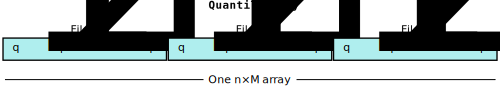
\includegraphics[width=\textwidth]{quantile_mem_layout.pdf}
  \caption{\label{fig:quantileMemLayout} How quantiles for each MPI
    process are stored in memory.}
\end{figure}

Let's now concentrate to the way quantiles are stored in memory. Each
MPI process must analyze a set of files, which is a subset of all the
files specified in the parameter file [REF XXX]. If the MPI process
needs to process $M$ files and extract $n$ quantiles from each of
them, then the most natural data structure in which to keep such
quantiles is a $n \times M$ bi-dimensional array (matrix). However, in
order to make things easier when we will implement the code to pass
such quantiles through MPI processes, we choose to use monodimensional
arrays that are indexed like a bi-dimensional one (see
Fig.~\ref{fig:quantileMemLayout}).

We declare two variables that will hold the quantiles: the first one
keeps the quantiles calculated for the files processed by the current
MPI process, while the second one will hold all the quantiles (this
will be used by the root process only):

\nwenddocs{}\nwbegincode{58}\sublabel{NW1IjHNk-49zmDD-2}\nwmargintag{{\nwtagstyle{}\subpageref{NW1IjHNk-49zmDD-2}}}\moddef{Variables used by \code{}phid\edoc{} and \code{}phisky\edoc{} in the main loop~{\nwtagstyle{}\subpageref{NW1IjHNk-49zmDD-1}}}\plusendmoddef\nwstartdeflinemarkup\nwusesondefline{\\{NW1IjHNk-Yygst-1}\\{NW1IjHNk-1UVtgN-1}}\nwprevnextdefs{NW1IjHNk-49zmDD-1}{NW1IjHNk-49zmDD-3}\nwenddeflinemarkup
QuantileArray, OverallQuantileArray : TDoubleArray;
\nwused{\\{NW1IjHNk-Yygst-1}\\{NW1IjHNk-1UVtgN-1}}\nwendcode{}\nwbegindocs{59}\nwdocspar

As we said above, the size of {\Tt{}QuantileArray\nwendquote} should be $n \times
M$, with $n$ the number of quantiles to compute and $M$ the number of
files processed by the current MPI process.
\nwenddocs{}\nwbegincode{60}\sublabel{NW1IjHNk-1w9u0s-1}\nwmargintag{{\nwtagstyle{}\subpageref{NW1IjHNk-1w9u0s-1}}}\moddef{Initialize the structures used to compress the TODs~{\nwtagstyle{}\subpageref{NW1IjHNk-1w9u0s-1}}}\endmoddef\nwstartdeflinemarkup\nwusesondefline{\\{NW1IjHNk-45bvtt-1}\\{NW1IjHNk-2ZGwF0-1}}\nwprevnextdefs{\relax}{NW1IjHNk-1w9u0s-2}\nwenddeflinemarkup
SetLength(QuantileArray, (\nwlinkedidentc{LastFileIdx}{NW1IjHNk-49zmDD-1} - \nwlinkedidentc{FirstFileIdx}{NW1IjHNk-49zmDD-1} + 1) * Length(\nwlinkedidentc{Configuration}{NW1IjHNk-COGTJ-1}.Quantiles));
\nwalsodefined{\\{NW1IjHNk-1w9u0s-2}}\nwused{\\{NW1IjHNk-45bvtt-1}\\{NW1IjHNk-2ZGwF0-1}}\nwidentuses{\\{{\nwixident{Configuration}}{Configuration}}\\{{\nwixident{FirstFileIdx}}{FirstFileIdx}}\\{{\nwixident{LastFileIdx}}{LastFileIdx}}}\nwindexuse{\nwixident{Configuration}}{Configuration}{NW1IjHNk-1w9u0s-1}\nwindexuse{\nwixident{FirstFileIdx}}{FirstFileIdx}{NW1IjHNk-1w9u0s-1}\nwindexuse{\nwixident{LastFileIdx}}{LastFileIdx}{NW1IjHNk-1w9u0s-1}\nwendcode{}\nwbegindocs{61}\nwdocspar

We are now ready to implement the main loop of the application:

\nwenddocs{}\nwbegincode{62}\sublabel{NW1IjHNk-3cFu7o-1}\nwmargintag{{\nwtagstyle{}\subpageref{NW1IjHNk-3cFu7o-1}}}\moddef{Apply Eq.~\eqref{eq:phiDDefinition} to the data in each pointing/temperature file~{\nwtagstyle{}\subpageref{NW1IjHNk-3cFu7o-1}}}\endmoddef\nwstartdeflinemarkup\nwusesondefline{\\{NW1IjHNk-45bvtt-1}}\nwenddeflinemarkup
for CurFileIdx := \nwlinkedidentc{FirstFileIdx}{NW1IjHNk-49zmDD-1} to \nwlinkedidentc{LastFileIdx}{NW1IjHNk-49zmDD-1} do
begin
    with \nwlinkedidentc{Configuration}{NW1IjHNk-COGTJ-1} do
    begin
        try
            \nwlinkedidentc{ProcessPointingFile}{NW1IjHNk-2azT0H-3}(PointingFileNames[CurFileIdx],
                                InputData, \nwlinkedidentc{PhiTod}{NW1IjHNk-COGTJ-3}, BinnedMap, HitMap);

            \nwlinkedidentc{AppendQuantiles}{NW1IjHNk-2zPeM0-4}(\nwlinkedidentc{PhiTod}{NW1IjHNk-COGTJ-3}.PhiD, \nwlinkedidentc{PhiTod}{NW1IjHNk-COGTJ-3}.Valid, \nwlinkedidentc{Configuration}{NW1IjHNk-COGTJ-1}.Quantiles,
                            QuantileArray, CurFileIdx - \nwlinkedidentc{FirstFileIdx}{NW1IjHNk-49zmDD-1});

            if \nwlinkedidentc{Configuration}{NW1IjHNk-COGTJ-1}.SaveTods then
                \nwlinkedidentc{SavePhiTod}{NW1IjHNk-2azT0H-4}(ConcatPaths([TodFilePath,
                    ChangeFileExt(ExtractFileName(PointingFileNames[CurFileIdx]),
                                  '-phid.fits')]),
                              \nwlinkedidentc{PhiTod}{NW1IjHNk-COGTJ-3});
        except
            on E : Exception do
                \nwlinkedidentc{Log}{NW1IjHNk-2DV5Ap-1}(Format('Unable to process file "%s" (%s), skipping…',
                           [PointingFileNames[CurFileIdx],
                            E.Message]));
        end;
    end;
end;
\nwused{\\{NW1IjHNk-45bvtt-1}}\nwidentuses{\\{{\nwixident{AppendQuantiles}}{AppendQuantiles}}\\{{\nwixident{Configuration}}{Configuration}}\\{{\nwixident{FirstFileIdx}}{FirstFileIdx}}\\{{\nwixident{LastFileIdx}}{LastFileIdx}}\\{{\nwixident{Log}}{Log}}\\{{\nwixident{PhiTod}}{PhiTod}}\\{{\nwixident{ProcessPointingFile}}{ProcessPointingFile}}\\{{\nwixident{SavePhiTod}}{SavePhiTod}}}\nwindexuse{\nwixident{AppendQuantiles}}{AppendQuantiles}{NW1IjHNk-3cFu7o-1}\nwindexuse{\nwixident{Configuration}}{Configuration}{NW1IjHNk-3cFu7o-1}\nwindexuse{\nwixident{FirstFileIdx}}{FirstFileIdx}{NW1IjHNk-3cFu7o-1}\nwindexuse{\nwixident{LastFileIdx}}{LastFileIdx}{NW1IjHNk-3cFu7o-1}\nwindexuse{\nwixident{Log}}{Log}{NW1IjHNk-3cFu7o-1}\nwindexuse{\nwixident{PhiTod}}{PhiTod}{NW1IjHNk-3cFu7o-1}\nwindexuse{\nwixident{ProcessPointingFile}}{ProcessPointingFile}{NW1IjHNk-3cFu7o-1}\nwindexuse{\nwixident{SavePhiTod}}{SavePhiTod}{NW1IjHNk-3cFu7o-1}\nwendcode{}\nwbegindocs{63}\nwdocspar

The program {\Tt{}phisky\nwendquote} uses a quite similar loop. Of course, in this
case we need to consider temperature files as well.
\nwenddocs{}\nwbegincode{64}\sublabel{NW1IjHNk-4Y2mxE-1}\nwmargintag{{\nwtagstyle{}\subpageref{NW1IjHNk-4Y2mxE-1}}}\moddef{Apply Eq.~\eqref{eq:phiSkyDefinition} to the data in each pointing/temperature file~{\nwtagstyle{}\subpageref{NW1IjHNk-4Y2mxE-1}}}\endmoddef\nwstartdeflinemarkup\nwusesondefline{\\{NW1IjHNk-2ZGwF0-1}}\nwenddeflinemarkup
for CurFileIdx := \nwlinkedidentc{FirstFileIdx}{NW1IjHNk-49zmDD-1} to \nwlinkedidentc{LastFileIdx}{NW1IjHNk-49zmDD-1} do
begin
    with \nwlinkedidentc{Configuration}{NW1IjHNk-COGTJ-1} do
    begin
        try
            \nwlinkedidentc{ProcessFilePair}{NW1IjHNk-3DL6qi-2}(PointingFileNames[CurFileIdx],
                            TemperatureFileNames[CurFileIdx],
                            InputData, \nwlinkedidentc{Configuration}{NW1IjHNk-COGTJ-1}.QualityFlagMask,
                            \nwlinkedidentc{PhiTod}{NW1IjHNk-COGTJ-3}, BinnedMap, HitMap);

            \nwlinkedidentc{AppendQuantiles}{NW1IjHNk-2zPeM0-4}(\nwlinkedidentc{PhiTod}{NW1IjHNk-COGTJ-3}.PhiSky, \nwlinkedidentc{PhiTod}{NW1IjHNk-COGTJ-3}.Valid, \nwlinkedidentc{Configuration}{NW1IjHNk-COGTJ-1}.Quantiles,
                            QuantileArray, CurFileIdx - \nwlinkedidentc{FirstFileIdx}{NW1IjHNk-49zmDD-1});

            if \nwlinkedidentc{Configuration}{NW1IjHNk-COGTJ-1}.SaveTods then
                \nwlinkedidentc{SavePhiTod}{NW1IjHNk-2azT0H-4}(ConcatPaths([TodFilePath,
                    ChangeFileExt(ExtractFileName(TemperatureFileNames[CurFileIdx]),
                                  '-phisky.fits')]),
                              \nwlinkedidentc{PhiTod}{NW1IjHNk-COGTJ-3});
        except
            on E : Exception do
                \nwlinkedidentc{Log}{NW1IjHNk-2DV5Ap-1}(Format('Unable to process files "%s" and "%s" (%s), skipping…',
                           [PointingFileNames[CurFileIdx],
                            TemperatureFileNames[CurFileIdx],
                            E.Message]));
        end;
    end;
end;
\nwused{\\{NW1IjHNk-2ZGwF0-1}}\nwidentuses{\\{{\nwixident{AppendQuantiles}}{AppendQuantiles}}\\{{\nwixident{Configuration}}{Configuration}}\\{{\nwixident{FirstFileIdx}}{FirstFileIdx}}\\{{\nwixident{LastFileIdx}}{LastFileIdx}}\\{{\nwixident{Log}}{Log}}\\{{\nwixident{PhiTod}}{PhiTod}}\\{{\nwixident{ProcessFilePair}}{ProcessFilePair}}\\{{\nwixident{SavePhiTod}}{SavePhiTod}}}\nwindexuse{\nwixident{AppendQuantiles}}{AppendQuantiles}{NW1IjHNk-4Y2mxE-1}\nwindexuse{\nwixident{Configuration}}{Configuration}{NW1IjHNk-4Y2mxE-1}\nwindexuse{\nwixident{FirstFileIdx}}{FirstFileIdx}{NW1IjHNk-4Y2mxE-1}\nwindexuse{\nwixident{LastFileIdx}}{LastFileIdx}{NW1IjHNk-4Y2mxE-1}\nwindexuse{\nwixident{Log}}{Log}{NW1IjHNk-4Y2mxE-1}\nwindexuse{\nwixident{PhiTod}}{PhiTod}{NW1IjHNk-4Y2mxE-1}\nwindexuse{\nwixident{ProcessFilePair}}{ProcessFilePair}{NW1IjHNk-4Y2mxE-1}\nwindexuse{\nwixident{SavePhiTod}}{SavePhiTod}{NW1IjHNk-4Y2mxE-1}\nwendcode{}\nwbegindocs{65}\nwdocspar

The variable {\Tt{}CurFileIdx\nwendquote} used in the two {\Tt{}for\nwendquote} loops above is
declared within the scope of the main block:

\nwenddocs{}\nwbegincode{66}\sublabel{NW1IjHNk-49zmDD-3}\nwmargintag{{\nwtagstyle{}\subpageref{NW1IjHNk-49zmDD-3}}}\moddef{Variables used by \code{}phid\edoc{} and \code{}phisky\edoc{} in the main loop~{\nwtagstyle{}\subpageref{NW1IjHNk-49zmDD-1}}}\plusendmoddef\nwstartdeflinemarkup\nwusesondefline{\\{NW1IjHNk-Yygst-1}\\{NW1IjHNk-1UVtgN-1}}\nwprevnextdefs{NW1IjHNk-49zmDD-2}{NW1IjHNk-49zmDD-4}\nwenddeflinemarkup
CurFileIdx : Integer;
\nwindexdefn{\nwixident{CurFileName}}{CurFileName}{NW1IjHNk-49zmDD-3}\eatline
\nwused{\\{NW1IjHNk-Yygst-1}\\{NW1IjHNk-1UVtgN-1}}\nwidentdefs{\\{{\nwixident{CurFileName}}{CurFileName}}}\nwendcode{}\nwbegindocs{67}\nwdocspar
\subsubsection{Saving the $\phid$ and $\phisky$ TODs}

The two programs save the information in the {\Tt{}\nwlinkedidentq{TPhiDTod}{NW1IjHNk-2dO5ki-3}\nwendquote} and
{\Tt{}\nwlinkedidentq{TPhiSkyTod}{NW1IjHNk-3VBxbc-3}\nwendquote} variable into a FITS file. In both cases, the file
contains just one binary table HDU and is created by the procedure
{\Tt{}\nwlinkedidentq{SavePhiTod}{NW1IjHNk-2azT0H-4}\nwendquote}, whose implementation of course differ between {\Tt{}phid\nwendquote}
and {\Tt{}phisky\nwendquote}.

\nwenddocs{}\nwbegincode{68}\sublabel{NW1IjHNk-2azT0H-4}\nwmargintag{{\nwtagstyle{}\subpageref{NW1IjHNk-2azT0H-4}}}\moddef{High-level functions for the \code{}phid\edoc{} program~{\nwtagstyle{}\subpageref{NW1IjHNk-2azT0H-1}}}\plusendmoddef\nwstartdeflinemarkup\nwusesondefline{\\{NW1IjHNk-Yygst-1}}\nwprevnextdefs{NW1IjHNk-2azT0H-3}{NW1IjHNk-2azT0H-5}\nwenddeflinemarkup
procedure \nwlinkedidentc{SavePhiTod}{NW1IjHNk-2azT0H-4}(const FileName : String;
                     const PhiDTod : \nwlinkedidentc{TPhiDTod}{NW1IjHNk-2dO5ki-3});
const
    FileColumns : Array[1..5] of Cfitsio.TColumn =
        ((Name: 'OBTTIME'; Count: 1; DataType: FitsTypeDouble;  UnitStr: ''),
         (Name: 'BSLD';    Count: 1; DataType: FitsTypeFloat;   UnitStr: 'K_CMB'),
         (Name: 'BMD';     Count: 1; DataType: FitsTypeFloat;   UnitStr: 'K_CMB'),
         (Name: 'PHID';    Count: 1; DataType: FitsTypeFloat;   UnitStr: 'K_CMB'),
         (Name: 'VALID';   Count: 1; DataType: FitsTypeLogical; UnitStr: ''));

var
    F : TFitsFile;

begin
    \nwlinkedidentc{Log}{NW1IjHNk-2DV5Ap-1}(Format('Saving %d values of φ_D into file %s…',
               [Length(PhiDTod.ObtTimes), FileName]));
    try
        \nwlinkedidentc{EnsurePathExists}{NW1IjHNk-2DV5Ap-2}(FileName);
        F := Cfitsio.CreateFile(FileName, Overwrite);
        try
            Cfitsio.CreateTable(F, BinaryTable, 0, FileColumns, 'PHID');
            Cfitsio.WriteComment(F, 'File created by the phid program');
            Cfitsio.WriteComment(F, 'Phid was compiled on ' +
                                        \{$i %date\} + ' ' + \{$i %time\});

            Cfitsio.WriteColumn(F, 1, 1, 1, PhiDTod.ObtTimes);
            Cfitsio.WriteColumn(F, 2, 1, 1, PhiDTod.BslD);
            Cfitsio.WriteColumn(F, 3, 1, 1, PhiDTod.BmD);
            Cfitsio.WriteColumn(F, 4, 1, 1, PhiDTod.PhiD);
            Cfitsio.WriteColumn(F, 5, 1, 1, PhiDTod.Valid);

            \nwlinkedidentc{Log}{NW1IjHNk-2DV5Ap-1}(Format('…done, file %s has been saved', [FileName]));
        finally
            Cfitsio.CloseFile(F);
        end;
    except
        on E : EFitsError do \nwlinkedidentc{Log}{NW1IjHNk-2DV5Ap-1}(Format('Unable to write file %s: %s',
                                        [FileName, E.message]));
    end;
end;
\nwindexdefn{\nwixident{SavePhiTod}}{SavePhiTod}{NW1IjHNk-2azT0H-4}\eatline
\nwused{\\{NW1IjHNk-Yygst-1}}\nwidentdefs{\\{{\nwixident{SavePhiTod}}{SavePhiTod}}}\nwidentuses{\\{{\nwixident{EnsurePathExists}}{EnsurePathExists}}\\{{\nwixident{Log}}{Log}}\\{{\nwixident{TPhiDTod}}{TPhiDTod}}}\nwindexuse{\nwixident{EnsurePathExists}}{EnsurePathExists}{NW1IjHNk-2azT0H-4}\nwindexuse{\nwixident{Log}}{Log}{NW1IjHNk-2azT0H-4}\nwindexuse{\nwixident{TPhiDTod}}{TPhiDTod}{NW1IjHNk-2azT0H-4}\nwendcode{}\nwbegindocs{69}The function {\Tt{}\nwlinkedidentq{EnsurePathExists}{NW1IjHNk-2DV5Ap-2}\nwendquote} is implemented in
Appendix~\ref{sec:FileUtilities}, and it creates the path needed to
save the file specified in its argument if needed (e.g., a call to
{\Tt{}\nwlinkedidentq{EnsurePathExists}{NW1IjHNk-2DV5Ap-2}('/path/test.fits')\nwendquote} will create the directory
\texttt{/path} if it does not exist).

\nwenddocs{}\nwbegincode{70}\sublabel{NW1IjHNk-3DL6qi-3}\nwmargintag{{\nwtagstyle{}\subpageref{NW1IjHNk-3DL6qi-3}}}\moddef{High-level functions for the \code{}phisky\edoc{} program~{\nwtagstyle{}\subpageref{NW1IjHNk-3DL6qi-1}}}\plusendmoddef\nwstartdeflinemarkup\nwusesondefline{\\{NW1IjHNk-1UVtgN-1}}\nwprevnextdefs{NW1IjHNk-3DL6qi-2}{NW1IjHNk-3DL6qi-4}\nwenddeflinemarkup
procedure \nwlinkedidentc{SavePhiTod}{NW1IjHNk-2azT0H-4}(const FileName : String;
                     const PhiSkyTod : \nwlinkedidentc{TPhiSkyTod}{NW1IjHNk-3VBxbc-3});
const
    FileColumns : Array[1..6] of Cfitsio.TColumn =
        ((Name: 'OBTTIME'; Count: 1; DataType: FitsTypeDouble;  UnitStr: ''),
         (Name: 'SLCONV';  Count: 1; DataType: FitsTypeFloat;   UnitStr: 'K_CMB'),
         (Name: 'MBCONV';  Count: 1; DataType: FitsTypeFloat;   UnitStr: 'K_CMB'),
         (Name: 'TSKY';    Count: 1; DataType: FitsTypeFloat;   UnitStr: 'K_CMB'),
         (Name: 'PHISKY';  Count: 1; DataType: FitsTypeFloat;   UnitStr: 'K_CMB'),
         (Name: 'VALID';   Count: 1; DataType: FitsTypeLogical; UnitStr: ''));

var
    F : TFitsFile;

begin
    \nwlinkedidentc{Log}{NW1IjHNk-2DV5Ap-1}(Format('Saving %d values of φ_sky into file %s',
               [Length(PhiSkyTod.ObtTimes), FileName]));
    try
        \nwlinkedidentc{EnsurePathExists}{NW1IjHNk-2DV5Ap-2}(FileName);
        F := Cfitsio.CreateFile(FileName, Overwrite);
        try
            Cfitsio.CreateTable(F, BinaryTable, 0, FileColumns, 'PHISKY');
            Cfitsio.WriteComment(F, 'File created by the phisky program');
            Cfitsio.WriteComment(F, 'Phisky was compiled on ' +
                                        \{$i %date\} + ' ' + \{$i %time\});
            Cfitsio.WriteColumn(F, 1, 1, 1, PhiSkyTod.ObtTimes);
            Cfitsio.WriteColumn(F, 2, 1, 1, PhiSkyTod.BslTsky);
            Cfitsio.WriteColumn(F, 3, 1, 1, PhiSkyTod.BmTsky);
            Cfitsio.WriteColumn(F, 4, 1, 1, PhiSkyTod.TskyMeas);
            Cfitsio.WriteColumn(F, 5, 1, 1, PhiSkyTod.PhiSky);
            Cfitsio.WriteColumn(F, 6, 1, 1, PhiSkyTod.Valid);
        finally
            Cfitsio.CloseFile(F);
        end;
    except
        on E : EFitsError do \nwlinkedidentc{Log}{NW1IjHNk-2DV5Ap-1}(Format('Unable to write file %s: %s',
                                        [FileName, E.message]));
    end;
end;
\nwused{\\{NW1IjHNk-1UVtgN-1}}\nwidentuses{\\{{\nwixident{EnsurePathExists}}{EnsurePathExists}}\\{{\nwixident{Log}}{Log}}\\{{\nwixident{SavePhiTod}}{SavePhiTod}}\\{{\nwixident{TPhiSkyTod}}{TPhiSkyTod}}}\nwindexuse{\nwixident{EnsurePathExists}}{EnsurePathExists}{NW1IjHNk-3DL6qi-3}\nwindexuse{\nwixident{Log}}{Log}{NW1IjHNk-3DL6qi-3}\nwindexuse{\nwixident{SavePhiTod}}{SavePhiTod}{NW1IjHNk-3DL6qi-3}\nwindexuse{\nwixident{TPhiSkyTod}}{TPhiSkyTod}{NW1IjHNk-3DL6qi-3}\nwendcode{}\nwbegindocs{71}\nwdocspar

\subsection{Compressing and saving the results}
\label{sec:dimensionalityreduction}

The $\phisky$ TODs generated by the program require much disk space
(of the same order of magnitude as the pointings, which means roughly
20\,GB/radiometer if saved in a compressed format) Therefore, the
code reduces the dimensionality of the TODs in two ways:
\begin{itemize}
\item Statistical quantities are computed for each OD, and only these
  are saved. This is still a TOD, but instead of having one row per
  sample, we have one row per OD.
\item The values of $\phisky$ are projected (binned) on a Healpix
  map.
\end{itemize}

The {\Tt{}\nwlinkedidentq{TPercentageArray}{NW1IjHNk-Ssbon-1}\nwendquote} type used in the definition of {\Tt{}Quantiles\nwendquote}
is an open array of integer numbers ({\Tt{}\nwlinkedidentq{TPercentage}{NW1IjHNk-Ssbon-1}\nwendquote}) representing a
percentage. We use this custom type instead of a {\Tt{}Integer\nwendquote} because
in this way its range is automatically checked by the compiler:

\nwenddocs{}\nwbegincode{72}\sublabel{NW1IjHNk-Ssbon-1}\nwmargintag{{\nwtagstyle{}\subpageref{NW1IjHNk-Ssbon-1}}}\moddef{Basic type definitions (shared between \code{}phisky\edoc{} and \code{}phid\edoc{})~{\nwtagstyle{}\subpageref{NW1IjHNk-Ssbon-1}}}\endmoddef\nwstartdeflinemarkup\nwusesondefline{\\{NW1IjHNk-Yygst-1}\\{NW1IjHNk-1UVtgN-1}}\nwprevnextdefs{\relax}{NW1IjHNk-Ssbon-2}\nwenddeflinemarkup
\nwlinkedidentc{TPercentage}{NW1IjHNk-Ssbon-1} = 0..100;
\nwlinkedidentc{TPercentageArray}{NW1IjHNk-Ssbon-1} = array of \nwlinkedidentc{TPercentage}{NW1IjHNk-Ssbon-1}; \{ Open array \}
\nwindexdefn{\nwixident{TPercentage}}{TPercentage}{NW1IjHNk-Ssbon-1}\nwindexdefn{\nwixident{TPercentageArray}}{TPercentageArray}{NW1IjHNk-Ssbon-1}\eatline
\nwalsodefined{\\{NW1IjHNk-Ssbon-2}}\nwused{\\{NW1IjHNk-Yygst-1}\\{NW1IjHNk-1UVtgN-1}}\nwidentdefs{\\{{\nwixident{TPercentage}}{TPercentage}}\\{{\nwixident{TPercentageArray}}{TPercentageArray}}}\nwendcode{}\nwbegindocs{73}\nwdocspar
We add a few useful new types as well:

\nwenddocs{}\nwbegincode{74}\sublabel{NW1IjHNk-Ssbon-2}\nwmargintag{{\nwtagstyle{}\subpageref{NW1IjHNk-Ssbon-2}}}\moddef{Basic type definitions (shared between \code{}phisky\edoc{} and \code{}phid\edoc{})~{\nwtagstyle{}\subpageref{NW1IjHNk-Ssbon-1}}}\plusendmoddef\nwstartdeflinemarkup\nwusesondefline{\\{NW1IjHNk-Yygst-1}\\{NW1IjHNk-1UVtgN-1}}\nwprevnextdefs{NW1IjHNk-Ssbon-1}{\relax}\nwenddeflinemarkup
\nwlinkedidentc{TStringArray}{NW1IjHNk-Ssbon-2} = array of String;  \{ Open array \}
TDoubleArray = array of Double;  \{ Open array \}
TBoolArray   = array of Boolean; \{ Open array \}
\nwindexdefn{\nwixident{TStringArray}}{TStringArray}{NW1IjHNk-Ssbon-2}\eatline
\nwused{\\{NW1IjHNk-Yygst-1}\\{NW1IjHNk-1UVtgN-1}}\nwidentdefs{\\{{\nwixident{TStringArray}}{TStringArray}}}\nwendcode{}\nwbegindocs{75}\nwdocspar
\nwenddocs{}\nwbegincode{76}\sublabel{NW1IjHNk-40nchE-1}\nwmargintag{{\nwtagstyle{}\subpageref{NW1IjHNk-40nchE-1}}}\moddef{Compress the $\phisky$ TODs and produce reduced TODs~{\nwtagstyle{}\subpageref{NW1IjHNk-40nchE-1}}}\endmoddef\nwstartdeflinemarkup\nwenddeflinemarkup
\{ No code here \}
\nwnotused{Compress the $\phisky$ TODs and produce reduced TODs}\nwendcode{}\nwbegindocs{77}\nwdocspar

\subsubsection{Producing statistics for each OD}

To compute the quantiles, we need a sorting procedure. Unfortunately,
Free Pascal does not provide a general-purpose sorting routine, so we
provide here our own implementation of the ``quick sort'' algorithm:

\nwenddocs{}\nwbegincode{78}\sublabel{NW1IjHNk-2zPeM0-3}\nwmargintag{{\nwtagstyle{}\subpageref{NW1IjHNk-2zPeM0-3}}}\moddef{General functions (shared between \code{}phisky\edoc{} and \code{}phid\edoc{})~{\nwtagstyle{}\subpageref{NW1IjHNk-2zPeM0-1}}}\plusendmoddef\nwstartdeflinemarkup\nwusesondefline{\\{NW1IjHNk-Yygst-1}\\{NW1IjHNk-1UVtgN-1}}\nwprevnextdefs{NW1IjHNk-2zPeM0-2}{NW1IjHNk-2zPeM0-4}\nwenddeflinemarkup
procedure \nwlinkedidentc{InPlaceQuickSort}{NW1IjHNk-2zPeM0-3}(var A : Array of Double; FirstIdx, LastIdx : Integer);
Var
    i, j : LongInt;
    tmp, pivot : Double;

Begin
    i := FirstIdx;
    j := LastIdx;
    pivot := A[(FirstIdx + LastIdx) div 2];
    repeat
        while pivot > A[i] do Inc(i);
        While pivot < A[j] do Dec(j);
        if i <= j then begin
            tmp := A[i];
            A[i] := A[j];
            A[j] := tmp;
            Inc(i);
            Dec(j);
        end;
    until i > j;
    if FirstIdx < j then \nwlinkedidentc{InPlaceQuickSort}{NW1IjHNk-2zPeM0-3}(A, FirstIdx, j);
    if i < LastIdx then \nwlinkedidentc{InPlaceQuickSort}{NW1IjHNk-2zPeM0-3}(A, i, LastIdx);
End;
\nwindexdefn{\nwixident{InPlaceQuickSort}}{InPlaceQuickSort}{NW1IjHNk-2zPeM0-3}\eatline
\nwused{\\{NW1IjHNk-Yygst-1}\\{NW1IjHNk-1UVtgN-1}}\nwidentdefs{\\{{\nwixident{InPlaceQuickSort}}{InPlaceQuickSort}}}\nwendcode{}\nwbegindocs{79}\nwdocspar
To save memory, the {\Tt{}\nwlinkedidentq{InPlaceQuickSort}{NW1IjHNk-2zPeM0-3}\nwendquote} (as its name suggests)
performs an in-place sorting, so that at the end of the call the
original ordering of the double array {\Tt{}A\nwendquote} is lost.

Before applying {\Tt{}\nwlinkedidentq{InPlaceQuickSort}{NW1IjHNk-2zPeM0-3}\nwendquote}, we need to filter out those
elements of the $\phisky$ array that contain invalid values.
Therefore, our implementation of the {\Tt{}\nwlinkedidentq{AppendQuantiles}{NW1IjHNk-2zPeM0-4}\nwendquote} function has
the following structure:

\nwenddocs{}\nwbegincode{80}\sublabel{NW1IjHNk-2zPeM0-4}\nwmargintag{{\nwtagstyle{}\subpageref{NW1IjHNk-2zPeM0-4}}}\moddef{General functions (shared between \code{}phisky\edoc{} and \code{}phid\edoc{})~{\nwtagstyle{}\subpageref{NW1IjHNk-2zPeM0-1}}}\plusendmoddef\nwstartdeflinemarkup\nwusesondefline{\\{NW1IjHNk-Yygst-1}\\{NW1IjHNk-1UVtgN-1}}\nwprevnextdefs{NW1IjHNk-2zPeM0-3}{NW1IjHNk-2zPeM0-5}\nwenddeflinemarkup
procedure \nwlinkedidentc{AppendQuantiles}{NW1IjHNk-2zPeM0-4}(const A : TDoubleArray;
                          const Valid : TBoolArray;
                          const Quantiles : \nwlinkedidentc{TPercentageArray}{NW1IjHNk-Ssbon-1};
                          var QuantileArray : TDoubleArray;
                          ChunkIdx : Integer);
var
    ValidValues : TDoubleArray;
    Idx, ValidIdx, QuantIdx : Integer;
    ValuesStr : String;
begin
    Assert(Length(A) = Length(Valid));
    \nwlinkedidentc{Log}{NW1IjHNk-2DV5Ap-1}(Format('Computing %d quantiles out of an array of %d elements…',
               [Length(Quantiles), Length(A)]));
    \LA{}Pick the valid values from \code{}A\edoc{} and store them into \code{}ValidValues\edoc{}~{\nwtagstyle{}\subpageref{NW1IjHNk-4bTEqj-1}}\RA{}
    \LA{}Sort \code{}ValidValues\edoc{} and compute the quantiles from it~{\nwtagstyle{}\subpageref{NW1IjHNk-1GZx1H-1}}\RA{}
    \nwlinkedidentc{Log}{NW1IjHNk-2DV5Ap-1}(Format('…the quantiles are %s.', [ValuesStr]));
end;
\nwindexdefn{\nwixident{AppendQuantiles}}{AppendQuantiles}{NW1IjHNk-2zPeM0-4}\eatline
\nwused{\\{NW1IjHNk-Yygst-1}\\{NW1IjHNk-1UVtgN-1}}\nwidentdefs{\\{{\nwixident{AppendQuantiles}}{AppendQuantiles}}}\nwidentuses{\\{{\nwixident{Log}}{Log}}\\{{\nwixident{TPercentageArray}}{TPercentageArray}}}\nwindexuse{\nwixident{Log}}{Log}{NW1IjHNk-2zPeM0-4}\nwindexuse{\nwixident{TPercentageArray}}{TPercentageArray}{NW1IjHNk-2zPeM0-4}\nwendcode{}\nwbegindocs{81}\nwdocspar
The purpose of the variable {\Tt{}ValidValues\nwendquote} is to hold a subset of the
{\Tt{}A\nwendquote} array which corresponds to those values whose twin element in
{\Tt{}Valid\nwendquote} (an array of Boolean values) is {\Tt{}True\nwendquote}:

\nwenddocs{}\nwbegincode{82}\sublabel{NW1IjHNk-4bTEqj-1}\nwmargintag{{\nwtagstyle{}\subpageref{NW1IjHNk-4bTEqj-1}}}\moddef{Pick the valid values from \code{}A\edoc{} and store them into \code{}ValidValues\edoc{}~{\nwtagstyle{}\subpageref{NW1IjHNk-4bTEqj-1}}}\endmoddef\nwstartdeflinemarkup\nwusesondefline{\\{NW1IjHNk-2zPeM0-4}}\nwenddeflinemarkup
SetLength(ValidValues, Length(A));
ValidIdx := Low(ValidValues);
for Idx := Low(A) to High(A) do
begin
    if Valid[Idx] then
    begin
        ValidValues[ValidIdx] := A[Idx];
        Inc(ValidIdx);
    end;
end;
if ValidIdx = Low(ValidValues) then
begin
    \nwlinkedidentc{Log}{NW1IjHNk-2DV5Ap-1}('…no valid values found for this OD, skipping the computation of quantiles');
    Exit;
end;

SetLength(ValidValues, ValidIdx);  \{ Truncate the tail of ValidValues \}
\nwlinkedidentc{Log}{NW1IjHNk-2DV5Ap-1}(Format('…%d valid values found…', [Length(ValidValues)]));
\nwused{\\{NW1IjHNk-2zPeM0-4}}\nwidentuses{\\{{\nwixident{Log}}{Log}}}\nwindexuse{\nwixident{Log}}{Log}{NW1IjHNk-4bTEqj-1}\nwendcode{}\nwbegindocs{83}\nwdocspar

Once {\Tt{}ValidValues\nwendquote} is initialized, computing the quantiles is a
matter of picking the right indexes in the array. We do not check for
those cases where the quantile falls in the middle between two values
(the {\Tt{}div\nwendquote} operation is an integer division and throws away any
remainder), because we feel that the loss of precision due to this
choice is negligible but makes the code considerably simpler.

\nwenddocs{}\nwbegincode{84}\sublabel{NW1IjHNk-1GZx1H-1}\nwmargintag{{\nwtagstyle{}\subpageref{NW1IjHNk-1GZx1H-1}}}\moddef{Sort \code{}ValidValues\edoc{} and compute the quantiles from it~{\nwtagstyle{}\subpageref{NW1IjHNk-1GZx1H-1}}}\endmoddef\nwstartdeflinemarkup\nwusesondefline{\\{NW1IjHNk-2zPeM0-4}}\nwenddeflinemarkup
                \nwlinkedidentc{InPlaceQuickSort}{NW1IjHNk-2zPeM0-3}(ValidValues, Low(ValidValues), High(ValidValues));
\nwlinkedidentc{Log}{NW1IjHNk-2DV5Ap-1}(Format('…values have been sorted, their range is [%.3e, %.3e]…',
           [ValidValues[Low(ValidValues)], ValidValues[High(ValidValues)]]));
Idx := ChunkIdx * Length(Quantiles);
ValuesStr := '';
for QuantIdx := Low(Quantiles) to High(Quantiles) do
begin
    QuantileArray[Idx + QuantIdx] :=
        ValidValues[(Quantiles[QuantIdx] * Length(ValidValues)) div 100];
    if ValuesStr <> '' then ValuesStr := ValuesStr + ', ';
    ValuesStr := ValuesStr + Format('%.3e (%d%%)',
                                    [QuantileArray[Idx + QuantIdx], Quantiles[QuantIdx]]);
end;
\nwused{\\{NW1IjHNk-2zPeM0-4}}\nwidentuses{\\{{\nwixident{InPlaceQuickSort}}{InPlaceQuickSort}}\\{{\nwixident{Log}}{Log}}}\nwindexuse{\nwixident{InPlaceQuickSort}}{InPlaceQuickSort}{NW1IjHNk-1GZx1H-1}\nwindexuse{\nwixident{Log}}{Log}{NW1IjHNk-1GZx1H-1}\nwendcode{}\nwbegindocs{85}\nwdocspar


\subsubsection{Projecting $\phid$ and $\phisky$ on a Healpix map}

Another way to condensate the amount of information enclosed in a set
of $\phid$/$\phisky$ TODs is to project their value on a map. Both
{\Tt{}phid\nwendquote} and {\Tt{}phisky\nwendquote} take advantage of a set of a Free Pascal
implementation of the Healpix pixelisation scheme to produce a FITS
file containing the binned map of $\phid$ and $\phisky$ values.

The two programs produce the maps via the following steps:
\begin{enumerate}
\item Each time a pointing file is processed and the $\phid$/$\phisky$
  TOD has been calculated, it is immediately projected onto a pair of
  ``local'' maps. The first map keeps track of the sum of the
  $\phid$/$\phisky$ values that have ``hit'' that pixel, while the
  second one keeps track of the number of hits per pixel. These maps
  are qualified as ``local'', as each MPI process keeps its own pair
  of maps.
\item When all the pointing files have been processed by all the MPI
  processes, a ``reduce'' operation is performed by the root process
  (with rank \#0), and all the binned maps and hit maps are summed
  together.
\item Dividing each pixel of the binned map by the corresponding value
  in the hit map produces a map of $\phid$/$\phisky$ values.
\end{enumerate}

Each process has two pairs of binned/hit maps: the first one is
actually used by each process ({\Tt{}BinnedMap\nwendquote} and {\Tt{}HitMap\nwendquote}), while
the second pair is only used by the root process to collect the result
of all the maps.

\nwenddocs{}\nwbegincode{86}\sublabel{NW1IjHNk-49zmDD-4}\nwmargintag{{\nwtagstyle{}\subpageref{NW1IjHNk-49zmDD-4}}}\moddef{Variables used by \code{}phid\edoc{} and \code{}phisky\edoc{} in the main loop~{\nwtagstyle{}\subpageref{NW1IjHNk-49zmDD-1}}}\plusendmoddef\nwstartdeflinemarkup\nwusesondefline{\\{NW1IjHNk-Yygst-1}\\{NW1IjHNk-1UVtgN-1}}\nwprevnextdefs{NW1IjHNk-49zmDD-3}{NW1IjHNk-49zmDD-5}\nwenddeflinemarkup
BinnedMap, HitMap : THealpixMap;
OverallBinnedMap, OverallHitMap : THealpixMap;
\nwused{\\{NW1IjHNk-Yygst-1}\\{NW1IjHNk-1UVtgN-1}}\nwendcode{}\nwbegindocs{87}\nwdocspar

These variables are initialized before the loop over the pointing
files starts. We initialize {\Tt{}OverallBinnedMap\nwendquote} and {\Tt{}OverallHitMap\nwendquote}
in every MPI process, even if only the root process will actually use
it, because in this way we turn off a few warnings that might be
issued by the Free Pascal compiler:
\nwenddocs{}\nwbegincode{88}\sublabel{NW1IjHNk-1w9u0s-2}\nwmargintag{{\nwtagstyle{}\subpageref{NW1IjHNk-1w9u0s-2}}}\moddef{Initialize the structures used to compress the TODs~{\nwtagstyle{}\subpageref{NW1IjHNk-1w9u0s-1}}}\plusendmoddef\nwstartdeflinemarkup\nwusesondefline{\\{NW1IjHNk-45bvtt-1}\\{NW1IjHNk-2ZGwF0-1}}\nwprevnextdefs{NW1IjHNk-1w9u0s-1}{\relax}\nwenddeflinemarkup
InitMap(\nwlinkedidentc{Configuration}{NW1IjHNk-COGTJ-1}.Nside, Ring, BinnedMap);
InitMap(\nwlinkedidentc{Configuration}{NW1IjHNk-COGTJ-1}.Nside, Ring, HitMap);

InitMap(\nwlinkedidentc{Configuration}{NW1IjHNk-COGTJ-1}.Nside, Ring, OverallBinnedMap);
InitMap(\nwlinkedidentc{Configuration}{NW1IjHNk-COGTJ-1}.Nside, Ring, OverallHitMap);
\nwused{\\{NW1IjHNk-45bvtt-1}\\{NW1IjHNk-2ZGwF0-1}}\nwidentuses{\\{{\nwixident{Configuration}}{Configuration}}}\nwindexuse{\nwixident{Configuration}}{Configuration}{NW1IjHNk-1w9u0s-2}\nwendcode{}\nwbegindocs{89}\nwdocspar

The function that is used to construct the binned and hit maps is
{\Tt{}\nwlinkedidentq{ProjectTodOntoMap}{NW1IjHNk-2zPeM0-5}\nwendquote}. It assumes that the {\Tt{}NSIDE\nwendquote} value used by
{\Tt{}BinnedMap\nwendquote} and {\Tt{}HitMap\nwendquote} is the same.
\nwenddocs{}\nwbegincode{90}\sublabel{NW1IjHNk-2zPeM0-5}\nwmargintag{{\nwtagstyle{}\subpageref{NW1IjHNk-2zPeM0-5}}}\moddef{General functions (shared between \code{}phisky\edoc{} and \code{}phid\edoc{})~{\nwtagstyle{}\subpageref{NW1IjHNk-2zPeM0-1}}}\plusendmoddef\nwstartdeflinemarkup\nwusesondefline{\\{NW1IjHNk-Yygst-1}\\{NW1IjHNk-1UVtgN-1}}\nwprevnextdefs{NW1IjHNk-2zPeM0-4}{NW1IjHNk-2zPeM0-6}\nwenddeflinemarkup
procedure \nwlinkedidentc{ProjectTodOntoMap}{NW1IjHNk-2zPeM0-5}(const Pointings : TDetectorPointings;
                            const Tod : TDoubleArray;
                            const Valid : TBoolArray;
                            var BinnedMap : THealpixMap;
                            var HitMap : THealpixMap);
var
    Idx : Integer;
    PixelIdx : Cardinal;

begin
    \nwlinkedidentc{Log}{NW1IjHNk-2DV5Ap-1}(Format('Projecting %d samples into a NSIDE=%d map…',
               [Length(Tod), BinnedMap.Resolution.Nside]));
    for Idx := Low(Tod) to High(Tod) do
    begin
        if Valid[Idx] then
        begin
            PixelIdx := AnglesToPix(BinnedMap, Pointings.Theta[Idx], Pointings.Phi[Idx]);
            BinnedMap.Pixels[PixelIdx] := BinnedMap.Pixels[PixelIdx] + Tod[Idx];
            HitMap.Pixels[PixelIdx] := HitMap.Pixels[PixelIdx] + 1.0;
        end;
    end;
    \nwlinkedidentc{Log}{NW1IjHNk-2DV5Ap-1}('…projection completed.');
end;
\nwindexdefn{\nwixident{ProjectTodOntoMap}}{ProjectTodOntoMap}{NW1IjHNk-2zPeM0-5}\eatline
\nwused{\\{NW1IjHNk-Yygst-1}\\{NW1IjHNk-1UVtgN-1}}\nwidentdefs{\\{{\nwixident{ProjectTodOntoMap}}{ProjectTodOntoMap}}}\nwidentuses{\\{{\nwixident{Log}}{Log}}}\nwindexuse{\nwixident{Log}}{Log}{NW1IjHNk-2zPeM0-5}\nwendcode{}\nwbegindocs{91}\nwdocspar
\subsubsection{Saving the reduced TODs and the maps}

\begin{figure}[tbf]
  \centering
  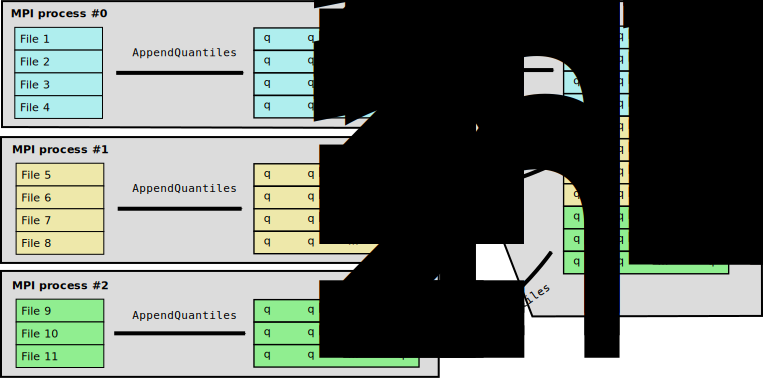
\includegraphics[width=\textwidth]{quantile_processing.pdf}
  \caption{\label{fig:gatherQuantiles} How quantiles are gathered
    together by the root MPI process. In this simple example we
    consider a run where a total of 11 files must be processed by 3
    MPI processes. Each MPI process computes its quantiles by calling
    \texttt{AppendQuantiles} iteratively. At the end of the process,
    all the MPI processes but the first send their results to the
    first process (the ``root'') by means of the procedure
    \texttt{GatherQuantiles}.}
\end{figure}

So far, the quantiles have been calculated by each MPI process for its
own files. It is time to gather them together and produce just one
file with all the quantiles (one row per file). This process is done
by the procedure {\Tt{}\nwlinkedidentq{GatherQuantiles}{NW1IjHNk-2zPeM0-6}\nwendquote}. Its role with respect to
{\Tt{}\nwlinkedidentq{AppendQuantiles}{NW1IjHNk-2zPeM0-4}\nwendquote} is sketched in Fig.~\ref{fig:gatherQuantiles}. The
implementation of {\Tt{}\nwlinkedidentq{GatherQuantiles}{NW1IjHNk-2zPeM0-6}\nwendquote} relies on the MPI functions
{\Tt{}Gather\nwendquote} and {\Tt{}Gatherv\nwendquote}.

\nwenddocs{}\nwbegincode{92}\sublabel{NW1IjHNk-2zPeM0-6}\nwmargintag{{\nwtagstyle{}\subpageref{NW1IjHNk-2zPeM0-6}}}\moddef{General functions (shared between \code{}phisky\edoc{} and \code{}phid\edoc{})~{\nwtagstyle{}\subpageref{NW1IjHNk-2zPeM0-1}}}\plusendmoddef\nwstartdeflinemarkup\nwusesondefline{\\{NW1IjHNk-Yygst-1}\\{NW1IjHNk-1UVtgN-1}}\nwprevnextdefs{NW1IjHNk-2zPeM0-5}{NW1IjHNk-2zPeM0-7}\nwenddeflinemarkup
procedure \nwlinkedidentc{GatherQuantiles}{NW1IjHNk-2zPeM0-6}(const LocalQuantiles : Array of Double;
                          out OverallQuantiles : TDoubleArray);
var
    Idx : Integer;
    BufLengths : Array of Integer;
    Displacements : Array of Integer;
    LocalBufLength : Array[1..1] of Integer;

begin
    \{ Retrieve the number of quantiles computed by each MPI process \}
    SetLength(BufLengths, Mpi.CommSize(Mpi.World));
    LocalBufLength[1] := Length(LocalQuantiles);
    Mpi.Gather(LocalBufLength, BufLengths, 0, Mpi.World);

    \{ Set up the array of displacements so that no holes will be left
      in OverallQuantiles \}
    SetLength(Displacements, Length(BufLengths));
    Displacements[0] := 0;
    for Idx := Low(BufLengths) to High(BufLengths) - 1 do
        Displacements[Idx + 1] := Displacements[Idx] + BufLengths[Idx];

    \{ Gather the quantiles from each MPI process to the root process \}
    SetLength(OverallQuantiles,
              Displacements[High(Displacements)] + BufLengths[High(BufLengths)]);
    Mpi.Gatherv(LocalQuantiles, OverallQuantiles, BufLengths,
                Displacements, 0, Mpi.World);
end;
\nwindexdefn{\nwixident{GatherQuantiles}}{GatherQuantiles}{NW1IjHNk-2zPeM0-6}\eatline
\nwused{\\{NW1IjHNk-Yygst-1}\\{NW1IjHNk-1UVtgN-1}}\nwidentdefs{\\{{\nwixident{GatherQuantiles}}{GatherQuantiles}}}\nwendcode{}\nwbegindocs{93}\nwdocspar
\nwenddocs{}\nwbegincode{94}\sublabel{NW1IjHNk-2zPeM0-7}\nwmargintag{{\nwtagstyle{}\subpageref{NW1IjHNk-2zPeM0-7}}}\moddef{General functions (shared between \code{}phisky\edoc{} and \code{}phid\edoc{})~{\nwtagstyle{}\subpageref{NW1IjHNk-2zPeM0-1}}}\plusendmoddef\nwstartdeflinemarkup\nwusesondefline{\\{NW1IjHNk-Yygst-1}\\{NW1IjHNk-1UVtgN-1}}\nwprevnextdefs{NW1IjHNk-2zPeM0-6}{NW1IjHNk-2zPeM0-8}\nwenddeflinemarkup
procedure SaveQuantileTOD(const FileName : String;
                          const Quantiles : \nwlinkedidentc{TPercentageArray}{NW1IjHNk-Ssbon-1};
                          const QuantileArray : TDoubleArray);
const
    PercentTableDef : Array[1..1] of Cfitsio.TColumn =
        ((Name: 'PERCENT'; Count: 1; DataType: FitsTypeShort; UnitStr: 'Percentage'));

var
    QuantileTableDef : Array of Cfitsio.TColumn;
    QuantIdx, Idx : Integer;
    F : TFitsFile;
    CurQuantiles : TDoubleArray;

begin
    SetLength(QuantileTableDef, Length(Quantiles));
    for QuantIdx := Low(QuantileTableDef) to High(QuantileTableDef) do
    begin
        with QuantileTableDef[QuantIdx] do
        begin
            Name := Format('Q%.3d', [Quantiles[QuantIdx]]);
            Count := 1;
            DataType := FitsTypeFloat;
            UnitStr := '';
        end;
    end;

    try
        \nwlinkedidentc{Log}{NW1IjHNk-2DV5Ap-1}(Format('Saving quantiles into FITS file "%s"…', [FileName]));
        F := Cfitsio.CreateFile(FileName, Overwrite);
        try
            CreateTable(F, BinaryTable, 0, PercentTableDef, 'PERCENTAGES');
            WriteColumn(F, 1, 1, 1, Quantiles);

            CreateTable(F, BinaryTable, 0, QuantileTableDef, 'QUANTILES');
            SetLength(CurQuantiles, Length(QuantileArray) div Length(Quantiles));
            for QuantIdx := 0 to Length(Quantiles) - 1 do
            begin
                for Idx := 0 to Length(CurQuantiles) - 1 do
                    CurQuantiles[Idx] := QuantileArray[Idx * Length(Quantiles) + QuantIdx];
                WriteColumn(F, 1 + QuantIdx, 1, 1, CurQuantiles);
            end;
        finally
            Cfitsio.CloseFile(F);
        end;
    except
        on E : Exception do \nwlinkedidentc{Log}{NW1IjHNk-2DV5Ap-1}(Format('Unable to write file "%s": %s',
                                       [FileName, E.Message]));
    end;
    \nwlinkedidentc{Log}{NW1IjHNk-2DV5Ap-1}(Format('…file "%s" saved.', [FileName]));
end;
\nwused{\\{NW1IjHNk-Yygst-1}\\{NW1IjHNk-1UVtgN-1}}\nwidentuses{\\{{\nwixident{Log}}{Log}}\\{{\nwixident{TPercentageArray}}{TPercentageArray}}}\nwindexuse{\nwixident{Log}}{Log}{NW1IjHNk-2zPeM0-7}\nwindexuse{\nwixident{TPercentageArray}}{TPercentageArray}{NW1IjHNk-2zPeM0-7}\nwendcode{}\nwbegindocs{95}%def

\nwenddocs{}\nwbegincode{96}\sublabel{NW1IjHNk-dyzak-1}\nwmargintag{{\nwtagstyle{}\subpageref{NW1IjHNk-dyzak-1}}}\moddef{Compress the TODs and produce reduced TODs~{\nwtagstyle{}\subpageref{NW1IjHNk-dyzak-1}}}\endmoddef\nwstartdeflinemarkup\nwusesondefline{\\{NW1IjHNk-45bvtt-1}\\{NW1IjHNk-2ZGwF0-1}}\nwprevnextdefs{\relax}{NW1IjHNk-dyzak-2}\nwenddeflinemarkup
\nwlinkedidentc{GatherQuantiles}{NW1IjHNk-2zPeM0-6}(QuantileArray, OverallQuantileArray);
if MpiRank = 0 then
begin
    \nwlinkedidentc{EnsurePathExists}{NW1IjHNk-2DV5Ap-2}(\nwlinkedidentc{Configuration}{NW1IjHNk-COGTJ-1}.QuantileTableFileName);
    SaveQuantileTOD(\nwlinkedidentc{Configuration}{NW1IjHNk-COGTJ-1}.QuantileTableFileName,
                    \nwlinkedidentc{Configuration}{NW1IjHNk-COGTJ-1}.Quantiles, OverallQuantileArray);
end;
\nwalsodefined{\\{NW1IjHNk-dyzak-2}}\nwused{\\{NW1IjHNk-45bvtt-1}\\{NW1IjHNk-2ZGwF0-1}}\nwidentuses{\\{{\nwixident{Configuration}}{Configuration}}\\{{\nwixident{EnsurePathExists}}{EnsurePathExists}}\\{{\nwixident{GatherQuantiles}}{GatherQuantiles}}}\nwindexuse{\nwixident{Configuration}}{Configuration}{NW1IjHNk-dyzak-1}\nwindexuse{\nwixident{EnsurePathExists}}{EnsurePathExists}{NW1IjHNk-dyzak-1}\nwindexuse{\nwixident{GatherQuantiles}}{GatherQuantiles}{NW1IjHNk-dyzak-1}\nwendcode{}\nwbegindocs{97}\nwdocspar

To produce the Healpix map containing the binned values of $\phid$ and
$\phisky$, we need to collect all the $N$ maps produced by each of the
$N$ MPI processes running. It is just a matter of calling the MPI
\texttt{reduce} function on the pixels of the local binned and hit
maps, and then normalize the binned map using the hit map:

\nwenddocs{}\nwbegincode{98}\sublabel{NW1IjHNk-dyzak-2}\nwmargintag{{\nwtagstyle{}\subpageref{NW1IjHNk-dyzak-2}}}\moddef{Compress the TODs and produce reduced TODs~{\nwtagstyle{}\subpageref{NW1IjHNk-dyzak-1}}}\plusendmoddef\nwstartdeflinemarkup\nwusesondefline{\\{NW1IjHNk-45bvtt-1}\\{NW1IjHNk-2ZGwF0-1}}\nwprevnextdefs{NW1IjHNk-dyzak-1}{\relax}\nwenddeflinemarkup
\nwlinkedidentc{Log}{NW1IjHNk-2DV5Ap-1}(Format('Reducing %d binned values…', [Length(BinnedMap.Pixels)]));
Mpi.Reduce(BinnedMap.Pixels, OverallBinnedMap.Pixels, MPI_SUM, 0, Mpi.World);
\nwlinkedidentc{Log}{NW1IjHNk-2DV5Ap-1}(Format('Reducing %d hit count pixels…', [Length(BinnedMap.Pixels)]));
Mpi.Reduce(HitMap.Pixels, OverallHitMap.Pixels, MPI_SUM, 0, Mpi.World);

if MpiRank = 0 then
begin
    for Idx := 0 to Length(BinnedMap.Pixels) - 1 do
    begin
        if OverallHitMap.Pixels[Idx] > 0 then
            OverallBinnedMap.Pixels[Idx] :=
                OverallBinnedMap.Pixels[Idx] / OverallHitMap.Pixels[Idx]
        else
            OverallBinnedMap.Pixels[Idx] := Healpix.Unseen;
    end;
end;
\nwused{\\{NW1IjHNk-45bvtt-1}\\{NW1IjHNk-2ZGwF0-1}}\nwidentuses{\\{{\nwixident{Log}}{Log}}}\nwindexuse{\nwixident{Log}}{Log}{NW1IjHNk-dyzak-2}\nwendcode{}\nwbegindocs{99}\nwdocspar

The map is now ready to be saved. We use the following format:
\nwenddocs{}\nwbegincode{100}\sublabel{NW1IjHNk-4NYge5-1}\nwmargintag{{\nwtagstyle{}\subpageref{NW1IjHNk-4NYge5-1}}}\moddef{General-purpose constants~{\nwtagstyle{}\subpageref{NW1IjHNk-4NYge5-1}}}\endmoddef\nwstartdeflinemarkup\nwusesondefline{\\{NW1IjHNk-Yygst-1}\\{NW1IjHNk-1UVtgN-1}}\nwenddeflinemarkup
    \nwlinkedidentc{MapColumns}{NW1IjHNk-4NYge5-1} : Array[1..2] of Cfitsio.TColumn =
        ((Name: 'AVGPHI'; Count: 1; DataType: FitsTypeFloat; UnitStr: ''),
         (Name: 'HITS';   Count: 1; DataType: FitsTypeLong;  UnitStr: ''));
\nwindexdefn{\nwixident{MapColumns}}{MapColumns}{NW1IjHNk-4NYge5-1}\eatline
\nwused{\\{NW1IjHNk-Yygst-1}\\{NW1IjHNk-1UVtgN-1}}\nwidentdefs{\\{{\nwixident{MapColumns}}{MapColumns}}}\nwendcode{}\nwbegindocs{101}\nwdocspar
Now to the code for saving the map. The {\Tt{}Healpix\nwendquote} unit already
provides a {\Tt{}WriteHealpixMap\nwendquote} procedure. However, this can be used
only for saving \emph{one} column, while here we're interested in
squeezing two columns in the same table. Fortunately, we do not have
to write low-level code, as the function {\Tt{}WriteHealpixKeywords\nwendquote}
already takes care of the burden of writing all the keywords needed by
the Healpix standard (e.g., \texttt{NSIDE}) in the current HDU:
\nwenddocs{}\nwbegincode{102}\sublabel{NW1IjHNk-4eqe6m-1}\nwmargintag{{\nwtagstyle{}\subpageref{NW1IjHNk-4eqe6m-1}}}\moddef{Save the reduced TODs~{\nwtagstyle{}\subpageref{NW1IjHNk-4eqe6m-1}}}\endmoddef\nwstartdeflinemarkup\nwusesondefline{\\{NW1IjHNk-45bvtt-1}\\{NW1IjHNk-2ZGwF0-1}}\nwenddeflinemarkup
if MpiRank = 0 then
begin
    \nwlinkedidentc{Log}{NW1IjHNk-2DV5Ap-1}(Format('Writing binned map in %s…', [\nwlinkedidentc{Configuration}{NW1IjHNk-COGTJ-1}.OutputMapFileName]));
    try
        \nwlinkedidentc{EnsurePathExists}{NW1IjHNk-2DV5Ap-2}(\nwlinkedidentc{Configuration}{NW1IjHNk-COGTJ-1}.OutputMapFileName);
        FitsFile := Cfitsio.CreateFile(\nwlinkedidentc{Configuration}{NW1IjHNk-COGTJ-1}.OutputMapFileName, Overwrite);
        try
            Cfitsio.CreateTable(FitsFile, BinaryTable, 0, \nwlinkedidentc{MapColumns}{NW1IjHNk-4NYge5-1}, 'PHIMAP');
            Healpix.WriteHealpixKeywords(FitsFile, OverallBinnedMap);
            Cfitsio.WriteColumn(FitsFile, 1, 1, 1, OverallBinnedMap.Pixels);
            Cfitsio.WriteColumn(FitsFile, 2, 1, 1, OverallHitMap.Pixels);
        finally
            Cfitsio.CloseFile(FitsFile);
        end;
        \nwlinkedidentc{Log}{NW1IjHNk-2DV5Ap-1}('…done, map has been written successfully');
    except
        on E : Exception do \nwlinkedidentc{Log}{NW1IjHNk-2DV5Ap-1}('…error, unable to write the map: ' + E.Message);
    end;
end;
\nwused{\\{NW1IjHNk-45bvtt-1}\\{NW1IjHNk-2ZGwF0-1}}\nwidentuses{\\{{\nwixident{Configuration}}{Configuration}}\\{{\nwixident{EnsurePathExists}}{EnsurePathExists}}\\{{\nwixident{Log}}{Log}}\\{{\nwixident{MapColumns}}{MapColumns}}}\nwindexuse{\nwixident{Configuration}}{Configuration}{NW1IjHNk-4eqe6m-1}\nwindexuse{\nwixident{EnsurePathExists}}{EnsurePathExists}{NW1IjHNk-4eqe6m-1}\nwindexuse{\nwixident{Log}}{Log}{NW1IjHNk-4eqe6m-1}\nwindexuse{\nwixident{MapColumns}}{MapColumns}{NW1IjHNk-4eqe6m-1}\nwendcode{}\nwbegindocs{103}\nwdocspar

The variable {\Tt{}FitsFile\nwendquote} is used both by {\Tt{}phid\nwendquote} and {\Tt{}phisky\nwendquote}, so
we declare it in the common section of the \texttt{var} block:
\nwenddocs{}\nwbegincode{104}\sublabel{NW1IjHNk-49zmDD-5}\nwmargintag{{\nwtagstyle{}\subpageref{NW1IjHNk-49zmDD-5}}}\moddef{Variables used by \code{}phid\edoc{} and \code{}phisky\edoc{} in the main loop~{\nwtagstyle{}\subpageref{NW1IjHNk-49zmDD-1}}}\plusendmoddef\nwstartdeflinemarkup\nwusesondefline{\\{NW1IjHNk-Yygst-1}\\{NW1IjHNk-1UVtgN-1}}\nwprevnextdefs{NW1IjHNk-49zmDD-4}{\relax}\nwenddeflinemarkup
FitsFile : TFitsFile;
\nwused{\\{NW1IjHNk-Yygst-1}\\{NW1IjHNk-1UVtgN-1}}\nwendcode{}\nwbegindocs{105}\nwdocspar

%%%%%%%%%%%%%%%%%%%%%%%%%%%%%%%%%%%%%%%%%%%%%%%%%%%%%%%%%%%%%%%%%%%%%%

\appendix

\section{Logging support}
\label{sec:Logging}

\nwenddocs{}\nwbegincode{106}\sublabel{NW1IjHNk-2DV5Ap-1}\nwmargintag{{\nwtagstyle{}\subpageref{NW1IjHNk-2DV5Ap-1}}}\moddef{Basic functions~{\nwtagstyle{}\subpageref{NW1IjHNk-2DV5Ap-1}}}\endmoddef\nwstartdeflinemarkup\nwusesondefline{\\{NW1IjHNk-Yygst-1}\\{NW1IjHNk-1UVtgN-1}}\nwprevnextdefs{\relax}{NW1IjHNk-2DV5Ap-2}\nwenddeflinemarkup
procedure \nwlinkedidentc{Log}{NW1IjHNk-2DV5Ap-1}(const Message : String);
var
    MpiRank : Integer;

begin
    MpiRank := Mpi.CommRank(Mpi.World);
    WriteLn(
                Format('[%s #%d] %s',
                       [FormatDateTime('YYYY/MM/DD tt', Now),
                        MpiRank,
                        Message]));
end;
\nwindexdefn{\nwixident{Log}}{Log}{NW1IjHNk-2DV5Ap-1}\eatline
\nwalsodefined{\\{NW1IjHNk-2DV5Ap-2}}\nwused{\\{NW1IjHNk-Yygst-1}\\{NW1IjHNk-1UVtgN-1}}\nwidentdefs{\\{{\nwixident{Log}}{Log}}}\nwendcode{}\nwbegindocs{107}\nwdocspar
\section{File utilities}
\label{sec:FileUtilities}

A very handy function to have when the programs need to save a file is
{\Tt{}\nwlinkedidentq{EnsurePathExists}{NW1IjHNk-2DV5Ap-2}\nwendquote}. It creates any missing directory in the path of
its argument, which can either be a file name or a path itself.

\nwenddocs{}\nwbegincode{108}\sublabel{NW1IjHNk-2DV5Ap-2}\nwmargintag{{\nwtagstyle{}\subpageref{NW1IjHNk-2DV5Ap-2}}}\moddef{Basic functions~{\nwtagstyle{}\subpageref{NW1IjHNk-2DV5Ap-1}}}\plusendmoddef\nwstartdeflinemarkup\nwusesondefline{\\{NW1IjHNk-Yygst-1}\\{NW1IjHNk-1UVtgN-1}}\nwprevnextdefs{NW1IjHNk-2DV5Ap-1}{\relax}\nwenddeflinemarkup
procedure \nwlinkedidentc{EnsurePathExists}{NW1IjHNk-2DV5Ap-2}(const FileName : String);
var
    Path : String;

begin
    Path := ExtractFilePath(ExpandFileName(FileName));
    if not ForceDirectories(Path) then
        raise Exception.CreateFmt('Unable to create the path "%s" ' +
                                  '(needed to save file "%s")',
                                  [Path, FileName]);
end;
\nwindexdefn{\nwixident{EnsurePathExists}}{EnsurePathExists}{NW1IjHNk-2DV5Ap-2}\eatline
\nwused{\\{NW1IjHNk-Yygst-1}\\{NW1IjHNk-1UVtgN-1}}\nwidentdefs{\\{{\nwixident{EnsurePathExists}}{EnsurePathExists}}}\nwendcode{}\nwbegindocs{109}\nwdocspar
\section{Reading INI files}
\ref{sec:parsingINIFiles}

To implement the procedure {\Tt{}\nwlinkedidentq{ReadConfiguration}{NW1IjHNk-2azT0H-5}\nwendquote}, we must have several
pieces of code at hand first. Free Pascal's large standard library
provides the {\Tt{}TIniFile\nwendquote}
class\footnote{\url{http://www.freepascal.org/docs-html/fcl/inifiles/tinifile.html}.},
which is a good starting point. But we also need some other low-level
functions. First, let's implement the procedure
{\Tt{}\nwlinkedidentq{GetAllValuesFromSection}{NW1IjHNk-2zPeM0-8}\nwendquote}, which will be used to retrieve the list
of ringsets from the sections \texttt{[Main ringsets]} and
\texttt{[Side ringsets]}. There is no method in {\Tt{}TIniFile\nwendquote} to
retrieve a list of values, so we use {\Tt{}TIniFile.ReadSection\nwendquote} to read
all the \emph{keys}, and then cycle over them to save its value into
{\Tt{}ValueList\nwendquote}.

\nwenddocs{}\nwbegincode{110}\sublabel{NW1IjHNk-2zPeM0-8}\nwmargintag{{\nwtagstyle{}\subpageref{NW1IjHNk-2zPeM0-8}}}\moddef{General functions (shared between \code{}phisky\edoc{} and \code{}phid\edoc{})~{\nwtagstyle{}\subpageref{NW1IjHNk-2zPeM0-1}}}\plusendmoddef\nwstartdeflinemarkup\nwusesondefline{\\{NW1IjHNk-Yygst-1}\\{NW1IjHNk-1UVtgN-1}}\nwprevnextdefs{NW1IjHNk-2zPeM0-7}{NW1IjHNk-2zPeM0-9}\nwenddeflinemarkup
procedure \nwlinkedidentc{GetAllValuesFromSection}{NW1IjHNk-2zPeM0-8}(IniFile : TIniFile;
                                  SectionName : String;
                                  var ValueList : \nwlinkedidentc{TStringArray}{NW1IjHNk-Ssbon-2});
var
    KeyList  : TStringList;
    Idx      : Integer;

begin
    KeyList := TStringList.Create;
    try
        IniFile.ReadSection(SectionName, KeyList);
        SetLength(ValueList, KeyList.Count);
        for Idx := 0 to KeyList.Count - 1 do
            ValueList[Idx] := (IniFile.ReadString(SectionName,
                                                  KeyList[Idx], ''));
    finally
        KeyList.Free;
    end;
end;
\nwindexdefn{\nwixident{GetAllValuesFromSection}}{GetAllValuesFromSection}{NW1IjHNk-2zPeM0-8}\eatline
\nwused{\\{NW1IjHNk-Yygst-1}\\{NW1IjHNk-1UVtgN-1}}\nwidentdefs{\\{{\nwixident{GetAllValuesFromSection}}{GetAllValuesFromSection}}}\nwidentuses{\\{{\nwixident{TStringArray}}{TStringArray}}}\nwindexuse{\nwixident{TStringArray}}{TStringArray}{NW1IjHNk-2zPeM0-8}\nwendcode{}\nwbegindocs{111}\nwdocspar
Parsing the list of pointing/temperature files is trickier, as in this
case the user might either list all the file names (in this case we
rely on {\Tt{}\nwlinkedidentq{GetAllValuesFromSection}{NW1IjHNk-2zPeM0-8}\nwendquote}) or use the shorthand provided by
{\Tt{}first{\_}index\nwendquote}/{\Tt{}last{\_}index\nwendquote}.

\nwenddocs{}\nwbegincode{112}\sublabel{NW1IjHNk-2zPeM0-9}\nwmargintag{{\nwtagstyle{}\subpageref{NW1IjHNk-2zPeM0-9}}}\moddef{General functions (shared between \code{}phisky\edoc{} and \code{}phid\edoc{})~{\nwtagstyle{}\subpageref{NW1IjHNk-2zPeM0-1}}}\plusendmoddef\nwstartdeflinemarkup\nwusesondefline{\\{NW1IjHNk-Yygst-1}\\{NW1IjHNk-1UVtgN-1}}\nwprevnextdefs{NW1IjHNk-2zPeM0-8}{NW1IjHNk-2zPeM0-A}\nwenddeflinemarkup
procedure \nwlinkedidentc{GetSequenceOfFiles}{NW1IjHNk-2zPeM0-9}(IniFile : TIniFile;
                             const SectName : String;
                             var FileNames : \nwlinkedidentc{TStringArray}{NW1IjHNk-Ssbon-2});
var
    FirstIdx, LastIdx, Idx : Integer;
    Template : String;

begin
    if IniFile.ValueExists(SectName, 'first_index') and
       IniFile.ValueExists(SectName, 'last_index') and
       IniFile.ValueExists(SectName, 'template') then
    begin
        FirstIdx := IniFile.ReadInteger(SectName, 'first_index', 0);
        LastIdx := IniFile.ReadInteger(SectName, 'last_index', 0);
        Template := IniFile.ReadString(SectName, 'template', '');

        SetLength(FileNames, LastIdx - FirstIdx + 1);
        for Idx := FirstIdx to LastIdx do
            FileNames[Idx - FirstIdx] := Format(Template, [Idx]);
    end else
        \nwlinkedidentc{GetAllValuesFromSection}{NW1IjHNk-2zPeM0-8}(IniFile, SectName, FileNames);
end;
\nwindexdefn{\nwixident{GetSequenceOfFiles}}{GetSequenceOfFiles}{NW1IjHNk-2zPeM0-9}\eatline
\nwused{\\{NW1IjHNk-Yygst-1}\\{NW1IjHNk-1UVtgN-1}}\nwidentdefs{\\{{\nwixident{GetSequenceOfFiles}}{GetSequenceOfFiles}}}\nwidentuses{\\{{\nwixident{GetAllValuesFromSection}}{GetAllValuesFromSection}}\\{{\nwixident{TStringArray}}{TStringArray}}}\nwindexuse{\nwixident{GetAllValuesFromSection}}{GetAllValuesFromSection}{NW1IjHNk-2zPeM0-9}\nwindexuse{\nwixident{TStringArray}}{TStringArray}{NW1IjHNk-2zPeM0-9}\nwendcode{}\nwbegindocs{113}\nwdocspar
Another piece of code we need is a procedure which parses the
comma-separated list of percentages associated to the {\Tt{}quantiles\nwendquote}
key (under the \texttt{[Output]} section).

\nwenddocs{}\nwbegincode{114}\sublabel{NW1IjHNk-2zPeM0-A}\nwmargintag{{\nwtagstyle{}\subpageref{NW1IjHNk-2zPeM0-A}}}\moddef{General functions (shared between \code{}phisky\edoc{} and \code{}phid\edoc{})~{\nwtagstyle{}\subpageref{NW1IjHNk-2zPeM0-1}}}\plusendmoddef\nwstartdeflinemarkup\nwusesondefline{\\{NW1IjHNk-Yygst-1}\\{NW1IjHNk-1UVtgN-1}}\nwprevnextdefs{NW1IjHNk-2zPeM0-9}{NW1IjHNk-2zPeM0-B}\nwenddeflinemarkup
procedure \nwlinkedidentc{GetPercentages}{NW1IjHNk-2zPeM0-A}(const InputStr : String;
                         out Percentages : \nwlinkedidentc{TPercentageArray}{NW1IjHNk-Ssbon-1});
var
    PercStrList : TStringList;
    Code : Word;
    Idx : Integer;

begin
    PercStrList := TStringList.Create;
    try
        ExtractStrings([','], [' ', #9], PChar(InputStr), PercStrList);
        SetLength(Percentages, PercStrList.Count);
        for Idx := 0 to PercStrList.Count - 1 do
        begin
            Val(PercStrList[Idx], Percentages[Idx], Code);
            if Code <> 0 then
                raise ERangeError(Format('"%s" is not a percentage',
                                         [PercStrList[Idx]]));
        end;
    finally
        PercStrList.Free;
    end;
end;
\nwindexdefn{\nwixident{GetPercentages}}{GetPercentages}{NW1IjHNk-2zPeM0-A}\eatline
\nwused{\\{NW1IjHNk-Yygst-1}\\{NW1IjHNk-1UVtgN-1}}\nwidentdefs{\\{{\nwixident{GetPercentages}}{GetPercentages}}}\nwidentuses{\\{{\nwixident{TPercentageArray}}{TPercentageArray}}}\nwindexuse{\nwixident{TPercentageArray}}{TPercentageArray}{NW1IjHNk-2zPeM0-A}\nwendcode{}\nwbegindocs{115}\nwdocspar
Now we are ready to implement the function {\Tt{}\nwlinkedidentq{ReadConfiguration}{NW1IjHNk-2azT0H-5}\nwendquote} for
{\Tt{}phid\nwendquote}. If the parameters of the solar CMB dipole are not provided,
then the Planck 2014 parameters will be used.

\nwenddocs{}\nwbegincode{116}\sublabel{NW1IjHNk-2azT0H-5}\nwmargintag{{\nwtagstyle{}\subpageref{NW1IjHNk-2azT0H-5}}}\moddef{High-level functions for the \code{}phid\edoc{} program~{\nwtagstyle{}\subpageref{NW1IjHNk-2azT0H-1}}}\plusendmoddef\nwstartdeflinemarkup\nwusesondefline{\\{NW1IjHNk-Yygst-1}}\nwprevnextdefs{NW1IjHNk-2azT0H-4}{NW1IjHNk-2azT0H-6}\nwenddeflinemarkup
procedure \nwlinkedidentc{ReadConfiguration}{NW1IjHNk-2azT0H-5}(const FileName : String;
                            out \nwlinkedidentc{Configuration}{NW1IjHNk-COGTJ-1} : \nwlinkedidentc{TPhiDConfiguration}{NW1IjHNk-2dO5ki-1});
var
    IniFile : TIniFile;
    ListOfPercentages : String;
begin
    IniFile := TIniFile.Create(FileName);
    try
        with \nwlinkedidentc{Configuration}{NW1IjHNk-COGTJ-1} do
        begin
            \nwlinkedidentc{GetAllValuesFromSection}{NW1IjHNk-2zPeM0-8}(IniFile, 'Main beam matrices', MbMatrixFileNames);
            \nwlinkedidentc{GetAllValuesFromSection}{NW1IjHNk-2zPeM0-8}(IniFile, 'Sidelobe matrices', SlMatrixFileNames);

            \nwlinkedidentc{GetSequenceOfFiles}{NW1IjHNk-2zPeM0-9}(IniFile, 'Pointings', PointingFileNames);

            SatelliteVelocityFileName :=
                IniFile.ReadString('Input', 'satellite_velocity_file', '');
            DipoleParams.DirTheta :=
                IniFile.ReadFloat('Input', 'dipole_dir_theta_ecl', 1.7656131194951572);
            DipoleParams.DirPhi :=
                IniFile.ReadFloat('Input', 'dipole_dir_phi_ecl', 2.9958896005735780);
            DipoleParams.SpeedMS :=
                IniFile.ReadFloat('Input', 'dipole_speed_m_s', 370082.2332);

            ListOfPercentages :=
                IniFile.ReadString('Output', 'quantiles', '25,50,75');
            \nwlinkedidentc{GetPercentages}{NW1IjHNk-2zPeM0-A}(ListOfPercentages, Quantiles);
            QuantileTableFileName := IniFile.ReadString('Output', 'quantiles_file_name', '');
            Nside := IniFile.ReadInteger('Output', 'map_nside', 64);
            if not Healpix.IsNsideValid(Nside) then
                raise Exception.CreateFmt('Invalid NSIDE value (%d)',
                                          [Nside]);

            OutputMapFileName :=
                IniFile.ReadString('Output', 'output_file_name', 'phi_d.fits');

            SaveTods := \nwlinkedidentc{ReadBoolean}{NW1IjHNk-2zPeM0-B}(IniFile, 'Output', 'save_tods', False);
            if SaveTods then
                TodFilePath :=
                    IniFile.ReadString('Output', 'tod_file_path', './');
        end;
    finally
        IniFile.Free;
    end;
end;
\nwindexdefn{\nwixident{ReadConfiguration}}{ReadConfiguration}{NW1IjHNk-2azT0H-5}\eatline
\nwused{\\{NW1IjHNk-Yygst-1}}\nwidentdefs{\\{{\nwixident{ReadConfiguration}}{ReadConfiguration}}}\nwidentuses{\\{{\nwixident{Configuration}}{Configuration}}\\{{\nwixident{GetAllValuesFromSection}}{GetAllValuesFromSection}}\\{{\nwixident{GetPercentages}}{GetPercentages}}\\{{\nwixident{GetSequenceOfFiles}}{GetSequenceOfFiles}}\\{{\nwixident{ReadBoolean}}{ReadBoolean}}\\{{\nwixident{TPhiDConfiguration}}{TPhiDConfiguration}}}\nwindexuse{\nwixident{Configuration}}{Configuration}{NW1IjHNk-2azT0H-5}\nwindexuse{\nwixident{GetAllValuesFromSection}}{GetAllValuesFromSection}{NW1IjHNk-2azT0H-5}\nwindexuse{\nwixident{GetPercentages}}{GetPercentages}{NW1IjHNk-2azT0H-5}\nwindexuse{\nwixident{GetSequenceOfFiles}}{GetSequenceOfFiles}{NW1IjHNk-2azT0H-5}\nwindexuse{\nwixident{ReadBoolean}}{ReadBoolean}{NW1IjHNk-2azT0H-5}\nwindexuse{\nwixident{TPhiDConfiguration}}{TPhiDConfiguration}{NW1IjHNk-2azT0H-5}\nwendcode{}\nwbegindocs{117}\nwdocspar
And here follows the same procedure for {\Tt{}phisky\nwendquote}:

\nwenddocs{}\nwbegincode{118}\sublabel{NW1IjHNk-3DL6qi-4}\nwmargintag{{\nwtagstyle{}\subpageref{NW1IjHNk-3DL6qi-4}}}\moddef{High-level functions for the \code{}phisky\edoc{} program~{\nwtagstyle{}\subpageref{NW1IjHNk-3DL6qi-1}}}\plusendmoddef\nwstartdeflinemarkup\nwusesondefline{\\{NW1IjHNk-1UVtgN-1}}\nwprevnextdefs{NW1IjHNk-3DL6qi-3}{NW1IjHNk-3DL6qi-5}\nwenddeflinemarkup
procedure \nwlinkedidentc{ReadConfiguration}{NW1IjHNk-2azT0H-5}(const FileName : String;
                            out \nwlinkedidentc{Configuration}{NW1IjHNk-COGTJ-1} : \nwlinkedidentc{TPhiSkyConfiguration}{NW1IjHNk-3VBxbc-1});
var
    IniFile : TIniFile;
    ListOfPercentages : String;
begin
    IniFile := TIniFile.Create(FileName);
    try
        with \nwlinkedidentc{Configuration}{NW1IjHNk-COGTJ-1} do
        begin
            \nwlinkedidentc{GetAllValuesFromSection}{NW1IjHNk-2zPeM0-8}(IniFile, 'Main ringsets', MbRingsetFileNames);
            \nwlinkedidentc{GetAllValuesFromSection}{NW1IjHNk-2zPeM0-8}(IniFile, 'Side ringsets', SlRingsetFileNames);

            \nwlinkedidentc{GetSequenceOfFiles}{NW1IjHNk-2zPeM0-9}(IniFile, 'Pointings', PointingFileNames);
            \nwlinkedidentc{GetSequenceOfFiles}{NW1IjHNk-2zPeM0-9}(IniFile, 'Temperatures', TemperatureFileNames);
            if Length(PointingFileNames) <> Length(TemperatureFileNames) then
                raise Exception.CreateFmt('# of pointing/temperature files differ (%d/%d)',
                                          [Length(PointingFileNames),
                                           Length(TemperatureFileNames)]);

            QualityFlagMask := IniFile.ReadInteger('Input', 'quality_flag_mask', 6111248);

            InterpolationOrder :=
                IniFile.ReadInteger('Output', 'interpolation_order', 5);
            ListOfPercentages :=
                IniFile.ReadString('Output', 'quantiles', '25,50,75');
            \nwlinkedidentc{GetPercentages}{NW1IjHNk-2zPeM0-A}(ListOfPercentages, Quantiles);
            QuantileTableFileName := IniFile.ReadString('Output', 'quantiles_file_name', '');
            Nside := IniFile.ReadInteger('Output', 'map_nside', 64);
            if not Healpix.IsNsideValid(Nside) then
                raise Exception.CreateFmt('Invalid NSIDE value (%d)',
                                          [Nside]);

            OutputMapFileName :=
                IniFile.ReadString('Output', 'output_file_name', 'phi_sky.fits');

            SaveTods := \nwlinkedidentc{ReadBoolean}{NW1IjHNk-2zPeM0-B}(IniFile, 'Output', 'save_tods', False);
            if SaveTods then
                TodFilePath :=
                    IniFile.ReadString('Output', 'tod_file_path', './');
        end;
    finally
        IniFile.Free;
    end;
end;
\nwindexdefn{\nwixident{ReadConfiguration}}{ReadConfiguration}{NW1IjHNk-3DL6qi-4}\eatline
\nwused{\\{NW1IjHNk-1UVtgN-1}}\nwidentdefs{\\{{\nwixident{ReadConfiguration}}{ReadConfiguration}}}\nwidentuses{\\{{\nwixident{Configuration}}{Configuration}}\\{{\nwixident{GetAllValuesFromSection}}{GetAllValuesFromSection}}\\{{\nwixident{GetPercentages}}{GetPercentages}}\\{{\nwixident{GetSequenceOfFiles}}{GetSequenceOfFiles}}\\{{\nwixident{ReadBoolean}}{ReadBoolean}}\\{{\nwixident{TPhiSkyConfiguration}}{TPhiSkyConfiguration}}}\nwindexuse{\nwixident{Configuration}}{Configuration}{NW1IjHNk-3DL6qi-4}\nwindexuse{\nwixident{GetAllValuesFromSection}}{GetAllValuesFromSection}{NW1IjHNk-3DL6qi-4}\nwindexuse{\nwixident{GetPercentages}}{GetPercentages}{NW1IjHNk-3DL6qi-4}\nwindexuse{\nwixident{GetSequenceOfFiles}}{GetSequenceOfFiles}{NW1IjHNk-3DL6qi-4}\nwindexuse{\nwixident{ReadBoolean}}{ReadBoolean}{NW1IjHNk-3DL6qi-4}\nwindexuse{\nwixident{TPhiSkyConfiguration}}{TPhiSkyConfiguration}{NW1IjHNk-3DL6qi-4}\nwendcode{}\nwbegindocs{119}\nwdocspar
To parse booleans, {\Tt{}TIniFile\nwendquote} provides the {\Tt{}ReadBool\nwendquote} method,
which is however quite limited (it only accepts {\Tt{}0\nwendquote}, which stands
for {\Tt{}false\nwendquote}, and {\Tt{}1\nwendquote}). So we provide a friendlier alternative in
the {\Tt{}\nwlinkedidentq{ReadBoolean}{NW1IjHNk-2zPeM0-B}\nwendquote} function, which we used above to parse the value
of the key {\Tt{}save{\_}tods\nwendquote} (in the \texttt{[Output]} section):

\nwenddocs{}\nwbegincode{120}\sublabel{NW1IjHNk-2zPeM0-B}\nwmargintag{{\nwtagstyle{}\subpageref{NW1IjHNk-2zPeM0-B}}}\moddef{General functions (shared between \code{}phisky\edoc{} and \code{}phid\edoc{})~{\nwtagstyle{}\subpageref{NW1IjHNk-2zPeM0-1}}}\plusendmoddef\nwstartdeflinemarkup\nwusesondefline{\\{NW1IjHNk-Yygst-1}\\{NW1IjHNk-1UVtgN-1}}\nwprevnextdefs{NW1IjHNk-2zPeM0-A}{NW1IjHNk-2zPeM0-C}\nwenddeflinemarkup
function \nwlinkedidentc{ReadBoolean}{NW1IjHNk-2zPeM0-B}(const IniFile : TIniFile;
                     const SectName : String;
                     const KeyName : String;
                     DefaultValue : Boolean) : Boolean;
var
    DefaultValStr : String;
    Value : String;

begin
    if DefaultValue then DefaultValStr := 'true' else DefaultValStr := 'false';

    Value := UpperCase(IniFile.ReadString(SectName, KeyName,
                                          DefaultValStr));
    if (Value = 'TRUE') or (Value = 'YES') or (Value = 'ON') then
        Exit(True)
    else if (Value = 'FALSE') or (Value = 'NO') or (Value = 'OFF') then
        Exit(False);

    \{ Unable to understand what the user wants, so stick with the default \}
    Exit(DefaultValue);
end;
\nwindexdefn{\nwixident{ReadBoolean}}{ReadBoolean}{NW1IjHNk-2zPeM0-B}\eatline
\nwused{\\{NW1IjHNk-Yygst-1}\\{NW1IjHNk-1UVtgN-1}}\nwidentdefs{\\{{\nwixident{ReadBoolean}}{ReadBoolean}}}\nwendcode{}\nwbegindocs{121}\nwdocspar
\subsection{Printing the configuration on the terminal}

In this section we implement the function {\Tt{}\nwlinkedidentq{PrintConfiguration}{NW1IjHNk-2azT0H-6}\nwendquote} for
both {\Tt{}phid\nwendquote} and {\Tt{}phisky\nwendquote}.

\nwenddocs{}\nwbegincode{122}\sublabel{NW1IjHNk-2azT0H-6}\nwmargintag{{\nwtagstyle{}\subpageref{NW1IjHNk-2azT0H-6}}}\moddef{High-level functions for the \code{}phid\edoc{} program~{\nwtagstyle{}\subpageref{NW1IjHNk-2azT0H-1}}}\plusendmoddef\nwstartdeflinemarkup\nwusesondefline{\\{NW1IjHNk-Yygst-1}}\nwprevnextdefs{NW1IjHNk-2azT0H-5}{NW1IjHNk-2azT0H-7}\nwenddeflinemarkup
procedure \nwlinkedidentc{PrintConfiguration}{NW1IjHNk-2azT0H-6}(const \nwlinkedidentc{Configuration}{NW1IjHNk-COGTJ-1} : \nwlinkedidentc{TPhiDConfiguration}{NW1IjHNk-2dO5ki-1});
begin
    with \nwlinkedidentc{Configuration}{NW1IjHNk-COGTJ-1} do
    begin
        \nwlinkedidentc{WriteFileNames}{NW1IjHNk-2zPeM0-C}('[Pointings]', PointingFileNames);
        \nwlinkedidentc{WriteFileNames}{NW1IjHNk-2zPeM0-C}('[Main beam matrices]', MbMatrixFileNames);
        \nwlinkedidentc{WriteFileNames}{NW1IjHNk-2zPeM0-C}('[Sidelobe matrices]', SlMatrixFileNames);

        WriteLn('[Input]');
        WriteLn('satellite_velocity = ', SatelliteVelocityFileName);
        WriteLn;

        WriteLn('[Output]');
        WriteLn('nside = ', Nside);
        WriteLn('output_file_name = ', OutputMapFileName);
        \nwlinkedidentc{WriteQuantiles}{NW1IjHNk-2zPeM0-D}('quantiles', Quantiles);
        WriteLn('quantiles_file_name', QuantileTableFileName);
        WriteLn('save_tods = ', SaveTods);
        if SaveTods then
            WriteLn('tod_file_path = ', TodFilePath);
    end;
end;
\nwindexdefn{\nwixident{PrintConfiguration}}{PrintConfiguration}{NW1IjHNk-2azT0H-6}\eatline
\nwused{\\{NW1IjHNk-Yygst-1}}\nwidentdefs{\\{{\nwixident{PrintConfiguration}}{PrintConfiguration}}}\nwidentuses{\\{{\nwixident{Configuration}}{Configuration}}\\{{\nwixident{TPhiDConfiguration}}{TPhiDConfiguration}}\\{{\nwixident{WriteFileNames}}{WriteFileNames}}\\{{\nwixident{WriteQuantiles}}{WriteQuantiles}}}\nwindexuse{\nwixident{Configuration}}{Configuration}{NW1IjHNk-2azT0H-6}\nwindexuse{\nwixident{TPhiDConfiguration}}{TPhiDConfiguration}{NW1IjHNk-2azT0H-6}\nwindexuse{\nwixident{WriteFileNames}}{WriteFileNames}{NW1IjHNk-2azT0H-6}\nwindexuse{\nwixident{WriteQuantiles}}{WriteQuantiles}{NW1IjHNk-2azT0H-6}\nwendcode{}\nwbegindocs{123}\nwdocspar
\nwenddocs{}\nwbegincode{124}\sublabel{NW1IjHNk-3DL6qi-5}\nwmargintag{{\nwtagstyle{}\subpageref{NW1IjHNk-3DL6qi-5}}}\moddef{High-level functions for the \code{}phisky\edoc{} program~{\nwtagstyle{}\subpageref{NW1IjHNk-3DL6qi-1}}}\plusendmoddef\nwstartdeflinemarkup\nwusesondefline{\\{NW1IjHNk-1UVtgN-1}}\nwprevnextdefs{NW1IjHNk-3DL6qi-4}{NW1IjHNk-3DL6qi-6}\nwenddeflinemarkup
procedure \nwlinkedidentc{PrintConfiguration}{NW1IjHNk-2azT0H-6}(const \nwlinkedidentc{Configuration}{NW1IjHNk-COGTJ-1} : \nwlinkedidentc{TPhiSkyConfiguration}{NW1IjHNk-3VBxbc-1});
begin
    with \nwlinkedidentc{Configuration}{NW1IjHNk-COGTJ-1} do
    begin
        \nwlinkedidentc{WriteFileNames}{NW1IjHNk-2zPeM0-C}('[Pointings]', PointingFileNames);
        \nwlinkedidentc{WriteFileNames}{NW1IjHNk-2zPeM0-C}('[Temperatures]', TemperatureFileNames);
        \nwlinkedidentc{WriteFileNames}{NW1IjHNk-2zPeM0-C}('[Main ringsets]', MbRingsetFileNames);
        \nwlinkedidentc{WriteFileNames}{NW1IjHNk-2zPeM0-C}('[Side ringsets]', SlRingsetFileNames);

        WriteLn('[Output]');
        WriteLn('interpolation_order = ', InterpolationOrder);
        WriteLn('nside = ', Nside);
        WriteLn('output_file_name = ', OutputMapFileName);
        \nwlinkedidentc{WriteQuantiles}{NW1IjHNk-2zPeM0-D}('quantiles', Quantiles);
        WriteLn('quantiles_file_name', QuantileTableFileName);
        WriteLn('save_tods = ', SaveTods);
        if SaveTods then
            WriteLn('tod_file_path = ', TodFilePath);
    end;
end;
\nwindexdefn{\nwixident{PrintConfiguration}}{PrintConfiguration}{NW1IjHNk-3DL6qi-5}\eatline
\nwused{\\{NW1IjHNk-1UVtgN-1}}\nwidentdefs{\\{{\nwixident{PrintConfiguration}}{PrintConfiguration}}}\nwidentuses{\\{{\nwixident{Configuration}}{Configuration}}\\{{\nwixident{TPhiSkyConfiguration}}{TPhiSkyConfiguration}}\\{{\nwixident{WriteFileNames}}{WriteFileNames}}\\{{\nwixident{WriteQuantiles}}{WriteQuantiles}}}\nwindexuse{\nwixident{Configuration}}{Configuration}{NW1IjHNk-3DL6qi-5}\nwindexuse{\nwixident{TPhiSkyConfiguration}}{TPhiSkyConfiguration}{NW1IjHNk-3DL6qi-5}\nwindexuse{\nwixident{WriteFileNames}}{WriteFileNames}{NW1IjHNk-3DL6qi-5}\nwindexuse{\nwixident{WriteQuantiles}}{WriteQuantiles}{NW1IjHNk-3DL6qi-5}\nwendcode{}\nwbegindocs{125}\nwdocspar
The two implementations of {\Tt{}\nwlinkedidentq{PrintConfiguration}{NW1IjHNk-2azT0H-6}\nwendquote} use
{\Tt{}\nwlinkedidentq{WriteFileNames}{NW1IjHNk-2zPeM0-C}\nwendquote} to write a list of file names on the screen and
{\Tt{}\nwlinkedidentq{WriteQuantiles}{NW1IjHNk-2zPeM0-D}\nwendquote} to write the list of quantiles to use in producing
the reduced TODs. The implementation of the former is fairly trivial:

\nwenddocs{}\nwbegincode{126}\sublabel{NW1IjHNk-2zPeM0-C}\nwmargintag{{\nwtagstyle{}\subpageref{NW1IjHNk-2zPeM0-C}}}\moddef{General functions (shared between \code{}phisky\edoc{} and \code{}phid\edoc{})~{\nwtagstyle{}\subpageref{NW1IjHNk-2zPeM0-1}}}\plusendmoddef\nwstartdeflinemarkup\nwusesondefline{\\{NW1IjHNk-Yygst-1}\\{NW1IjHNk-1UVtgN-1}}\nwprevnextdefs{NW1IjHNk-2zPeM0-B}{NW1IjHNk-2zPeM0-D}\nwenddeflinemarkup
procedure \nwlinkedidentc{WriteFileNames}{NW1IjHNk-2zPeM0-C}(const SectName : String;
                         const NameList : \nwlinkedidentc{TStringArray}{NW1IjHNk-Ssbon-2});
var
    Idx : Integer;

begin
    WriteLn(SectName);
    for Idx := 0 to Length(NameList) - 1 do
        WriteLn(Format('file_name_%.4d = %s',
                       [Idx, NameList[Idx]]));

    WriteLn;
end;
\nwindexdefn{\nwixident{WriteFileNames}}{WriteFileNames}{NW1IjHNk-2zPeM0-C}\eatline
\nwused{\\{NW1IjHNk-Yygst-1}\\{NW1IjHNk-1UVtgN-1}}\nwidentdefs{\\{{\nwixident{WriteFileNames}}{WriteFileNames}}}\nwidentuses{\\{{\nwixident{TStringArray}}{TStringArray}}}\nwindexuse{\nwixident{TStringArray}}{TStringArray}{NW1IjHNk-2zPeM0-C}\nwendcode{}\nwbegindocs{127}\nwdocspar
The procedure {\Tt{}\nwlinkedidentq{WriteQuantiles}{NW1IjHNk-2zPeM0-D}\nwendquote} writes a nicely formatted list of
comma-separated percentages on the standard output. It is just called
once, but moving this code out of {\Tt{}\nwlinkedidentq{PrintConfiguration}{NW1IjHNk-2azT0H-6}\nwendquote} improves the
readability of the latter.

\nwenddocs{}\nwbegincode{128}\sublabel{NW1IjHNk-2zPeM0-D}\nwmargintag{{\nwtagstyle{}\subpageref{NW1IjHNk-2zPeM0-D}}}\moddef{General functions (shared between \code{}phisky\edoc{} and \code{}phid\edoc{})~{\nwtagstyle{}\subpageref{NW1IjHNk-2zPeM0-1}}}\plusendmoddef\nwstartdeflinemarkup\nwusesondefline{\\{NW1IjHNk-Yygst-1}\\{NW1IjHNk-1UVtgN-1}}\nwprevnextdefs{NW1IjHNk-2zPeM0-C}{\relax}\nwenddeflinemarkup
procedure \nwlinkedidentc{WriteQuantiles}{NW1IjHNk-2zPeM0-D}(const KeyName : String;
                         const Quantiles : \nwlinkedidentc{TPercentageArray}{NW1IjHNk-Ssbon-1});
var
    Idx : Integer;

begin
    Write(KeyName, ' = ');
    for Idx := 0 to Length(Quantiles) - 1 do
    begin
        Write(Quantiles[Idx]);
        if Idx < High(Quantiles) then
            Write(', ')
        else
            WriteLn;
    end;
end;
\nwindexdefn{\nwixident{WriteQuantiles}}{WriteQuantiles}{NW1IjHNk-2zPeM0-D}\eatline
\nwused{\\{NW1IjHNk-Yygst-1}\\{NW1IjHNk-1UVtgN-1}}\nwidentdefs{\\{{\nwixident{WriteQuantiles}}{WriteQuantiles}}}\nwidentuses{\\{{\nwixident{TPercentageArray}}{TPercentageArray}}}\nwindexuse{\nwixident{TPercentageArray}}{TPercentageArray}{NW1IjHNk-2zPeM0-D}\nwendcode{}\nwbegindocs{129}\nwdocspar
\section{Other helper functions}

\subsection{Loading sets of convolution matrices}

Here is a straightforward implementation of the procedure
{\Tt{}\nwlinkedidentq{LoadConvolutionMatrices}{NW1IjHNk-2azT0H-7}\nwendquote}.

\nwenddocs{}\nwbegincode{130}\sublabel{NW1IjHNk-2azT0H-7}\nwmargintag{{\nwtagstyle{}\subpageref{NW1IjHNk-2azT0H-7}}}\moddef{High-level functions for the \code{}phid\edoc{} program~{\nwtagstyle{}\subpageref{NW1IjHNk-2azT0H-1}}}\plusendmoddef\nwstartdeflinemarkup\nwusesondefline{\\{NW1IjHNk-Yygst-1}}\nwprevnextdefs{NW1IjHNk-2azT0H-6}{NW1IjHNk-2azT0H-8}\nwenddeflinemarkup
procedure \nwlinkedidentc{LoadConvolutionMatrices}{NW1IjHNk-2azT0H-7}(const FileNames : \nwlinkedidentc{TStringArray}{NW1IjHNk-Ssbon-2};
                                  out Matrices : TConvMatrixArray);
var
    Idx : Integer;
    \nwlinkedidentc{CurFileName}{NW1IjHNk-49zmDD-3} : String;

begin
    SetLength(Matrices, Length(FileNames));
    for Idx := 0 to Length(FileNames) - 1 do
    begin
        \nwlinkedidentc{CurFileName}{NW1IjHNk-49zmDD-3} := FileNames[Idx];
        \nwlinkedidentc{Log}{NW1IjHNk-2DV5Ap-1}(Format('Reading file %s', [\nwlinkedidentc{CurFileName}{NW1IjHNk-49zmDD-3}]));
        LoadConvolutionMatrix(\nwlinkedidentc{CurFileName}{NW1IjHNk-49zmDD-3}, Matrices[Idx]);
    end;
end;
\nwindexdefn{\nwixident{LoadConvolutionMatrices}}{LoadConvolutionMatrices}{NW1IjHNk-2azT0H-7}\eatline
\nwused{\\{NW1IjHNk-Yygst-1}}\nwidentdefs{\\{{\nwixident{LoadConvolutionMatrices}}{LoadConvolutionMatrices}}}\nwidentuses{\\{{\nwixident{CurFileName}}{CurFileName}}\\{{\nwixident{Log}}{Log}}\\{{\nwixident{TStringArray}}{TStringArray}}}\nwindexuse{\nwixident{CurFileName}}{CurFileName}{NW1IjHNk-2azT0H-7}\nwindexuse{\nwixident{Log}}{Log}{NW1IjHNk-2azT0H-7}\nwindexuse{\nwixident{TStringArray}}{TStringArray}{NW1IjHNk-2azT0H-7}\nwendcode{}\nwbegindocs{131}\nwdocspar
\nwenddocs{}\nwbegincode{132}\sublabel{NW1IjHNk-2azT0H-8}\nwmargintag{{\nwtagstyle{}\subpageref{NW1IjHNk-2azT0H-8}}}\moddef{High-level functions for the \code{}phid\edoc{} program~{\nwtagstyle{}\subpageref{NW1IjHNk-2azT0H-1}}}\plusendmoddef\nwstartdeflinemarkup\nwusesondefline{\\{NW1IjHNk-Yygst-1}}\nwprevnextdefs{NW1IjHNk-2azT0H-7}{\relax}\nwenddeflinemarkup
procedure \nwlinkedidentc{SumConvMatricesIntensities}{NW1IjHNk-2azT0H-8}(const Matrices : TConvMatrixArray;
                                     const SolSysVelEcl : TVector;
                                     const SatVel : TSatelliteVelocities;
                                     const Pointings : TDetectorPointings;
                                     var DestVector : TDoubleArray);
var
    MatIdx, Idx : Integer;

begin
    SetLength(DestVector, Length(Pointings.Theta));
    for Idx := 0 to Length(DestVector) - 1 do
        DestVector[Idx] := 0.0;

    for MatIdx := 0 to Length(Matrices) - 1 do
    begin
        \nwlinkedidentc{Log}{NW1IjHNk-2DV5Ap-1}(Format('Applying convolution matrix %d/%d', [Idx + 1, Length(Matrices)]));
        for Idx := 0 to Length(Pointings.Theta) - 1 do
            DestVector[Idx] := DestVector[Idx] +
                Convolve(Matrices[MatIdx], SolSysVelEcl, SatVel,
                         Pointings.ObtTimes[Idx],
                         Pointings.Theta[Idx], Pointings.Phi[Idx], Pointings.Psi[Idx]);
    end;
end;
\nwindexdefn{\nwixident{SumConvMatricesIntensities}}{SumConvMatricesIntensities}{NW1IjHNk-2azT0H-8}\eatline
\nwused{\\{NW1IjHNk-Yygst-1}}\nwidentdefs{\\{{\nwixident{SumConvMatricesIntensities}}{SumConvMatricesIntensities}}}\nwidentuses{\\{{\nwixident{Log}}{Log}}}\nwindexuse{\nwixident{Log}}{Log}{NW1IjHNk-2azT0H-8}\nwendcode{}\nwbegindocs{133}\nwdocspar
\subsection{Loading sets of ringsets}
\label{sec:LoadingSetsOfRingsets}

Here we provide a straightforward implementation of the procedure
{\Tt{}\nwlinkedidentq{LoadRingsets}{NW1IjHNk-3DL6qi-6}\nwendquote}.

\nwenddocs{}\nwbegincode{134}\sublabel{NW1IjHNk-3DL6qi-6}\nwmargintag{{\nwtagstyle{}\subpageref{NW1IjHNk-3DL6qi-6}}}\moddef{High-level functions for the \code{}phisky\edoc{} program~{\nwtagstyle{}\subpageref{NW1IjHNk-3DL6qi-1}}}\plusendmoddef\nwstartdeflinemarkup\nwusesondefline{\\{NW1IjHNk-1UVtgN-1}}\nwprevnextdefs{NW1IjHNk-3DL6qi-5}{NW1IjHNk-3DL6qi-7}\nwenddeflinemarkup
procedure \nwlinkedidentc{LoadRingsets}{NW1IjHNk-3DL6qi-6}(const FileNames : \nwlinkedidentc{TStringArray}{NW1IjHNk-Ssbon-2};
                       InterpolationOrder : Integer;
                       out Ringsets : TRingsetArray);
var
    Idx : Integer;
    \nwlinkedidentc{CurFileName}{NW1IjHNk-49zmDD-3} : String;

begin
    SetLength(Ringsets, Length(FileNames));
    for Idx := 0 to Length(FileNames) - 1 do
    begin
        \nwlinkedidentc{CurFileName}{NW1IjHNk-49zmDD-3} := FileNames[Idx];
        \nwlinkedidentc{Log}{NW1IjHNk-2DV5Ap-1}(Format('Reading file %s', [\nwlinkedidentc{CurFileName}{NW1IjHNk-49zmDD-3}]));
        LoadRingsetFromFile(\nwlinkedidentc{CurFileName}{NW1IjHNk-49zmDD-3},
                            InterpolationOrder,
                            Ringsets[Idx]);
    end;
end;
\nwindexdefn{\nwixident{LoadRingsets}}{LoadRingsets}{NW1IjHNk-3DL6qi-6}\eatline
\nwused{\\{NW1IjHNk-1UVtgN-1}}\nwidentdefs{\\{{\nwixident{LoadRingsets}}{LoadRingsets}}}\nwidentuses{\\{{\nwixident{CurFileName}}{CurFileName}}\\{{\nwixident{Log}}{Log}}\\{{\nwixident{TStringArray}}{TStringArray}}}\nwindexuse{\nwixident{CurFileName}}{CurFileName}{NW1IjHNk-3DL6qi-6}\nwindexuse{\nwixident{Log}}{Log}{NW1IjHNk-3DL6qi-6}\nwindexuse{\nwixident{TStringArray}}{TStringArray}{NW1IjHNk-3DL6qi-6}\nwendcode{}\nwbegindocs{135}\nwdocspar
We need a function which sums all the intensities of a set of
ringsets, too. This is provided by the {\Tt{}\nwlinkedidentq{SumRingsetIntensities}{NW1IjHNk-3DL6qi-7}\nwendquote}
procedure. It uses a callback, {\Tt{}UpdateUserAboutStatus\nwendquote}, to show how
much of the TOD has been processed so far. This is useful, as the
function {\Tt{}\nwlinkedidentq{SumRingsetIntensities}{NW1IjHNk-3DL6qi-7}\nwendquote} is going to take a lot of time to
complete when {\Tt{}phisky\nwendquote} is run on real data!

\nwenddocs{}\nwbegincode{136}\sublabel{NW1IjHNk-3DL6qi-7}\nwmargintag{{\nwtagstyle{}\subpageref{NW1IjHNk-3DL6qi-7}}}\moddef{High-level functions for the \code{}phisky\edoc{} program~{\nwtagstyle{}\subpageref{NW1IjHNk-3DL6qi-1}}}\plusendmoddef\nwstartdeflinemarkup\nwusesondefline{\\{NW1IjHNk-1UVtgN-1}}\nwprevnextdefs{NW1IjHNk-3DL6qi-6}{NW1IjHNk-3DL6qi-8}\nwenddeflinemarkup
procedure UpdateUserAboutStatus(Idx, NumOfElements : Integer; Data : Pointer);
var
    Percentage : Real;

begin
    if NumOfElements > 0 then
        Percentage := (Idx * 100.0) / (NumOfElements - 1)
    else
        Percentage := 100.0;

    \nwlinkedidentc{Log}{NW1IjHNk-2DV5Ap-1}(Format('   Ringset application: %d/%d (%.1f%%)',
               [Idx + 1, NumOfElements, Percentage]));
end;

procedure \nwlinkedidentc{SumRingsetIntensities}{NW1IjHNk-3DL6qi-7}(const Ringsets : TRingsetArray;
                                const Pointings : TDetectorPointings;
                                var DestVector : TDoubleArray);
const
    LogUpdateDelayInMs = 30000.0; \{ = 30 s \}
var
    Idx : Integer;
begin
    SetLength(DestVector, Length(Pointings.Theta));
    for Idx := 0 to Length(DestVector) - 1 do
        DestVector[Idx] := 0.0;

    for Idx := 0 to Length(Ringsets) - 1 do
    begin
        \nwlinkedidentc{Log}{NW1IjHNk-2DV5Ap-1}(Format('Applying ringset %d/%d', [Idx + 1, Length(Ringsets)]));
        GetRingsetIntensities(Ringsets[Idx], Pointings.Theta,
                              Pointings.Phi, Pointings.Psi,
                              DestVector, AddElements,
                              @UpdateUserAboutStatus, LogUpdateDelayInMs, nil);
    end;
end;
\nwindexdefn{\nwixident{SumRingsetIntensities}}{SumRingsetIntensities}{NW1IjHNk-3DL6qi-7}\eatline
\nwused{\\{NW1IjHNk-1UVtgN-1}}\nwidentdefs{\\{{\nwixident{SumRingsetIntensities}}{SumRingsetIntensities}}}\nwidentuses{\\{{\nwixident{Log}}{Log}}}\nwindexuse{\nwixident{Log}}{Log}{NW1IjHNk-3DL6qi-7}\nwendcode{}\nwbegindocs{137}\nwdocspar
We provide here an implementation of {\Tt{}\nwlinkedidentq{MemoryUsed}{NW1IjHNk-3DL6qi-8}\nwendquote}, which is used by
{\Tt{}phisky\nwendquote} to quantify how much memory is used by the ringsets. The
unit {\Tt{}Ringsets\nwendquote} already provides a function {\Tt{}BytesUsed\nwendquote}, which
returns the number of bytes used by a {\Tt{}TRingset\nwendquote} record. We wrap
this into a more user-frendly function, which calculates the memory
needed by \emph{all} the ringsets in a {\Tt{}\nwlinkedidentq{TPhiSkyInputData}{NW1IjHNk-3VBxbc-2}\nwendquote} record and
the $\Tsky$ map, and formats the result using the proper measure unit.

\nwenddocs{}\nwbegincode{138}\sublabel{NW1IjHNk-3DL6qi-8}\nwmargintag{{\nwtagstyle{}\subpageref{NW1IjHNk-3DL6qi-8}}}\moddef{High-level functions for the \code{}phisky\edoc{} program~{\nwtagstyle{}\subpageref{NW1IjHNk-3DL6qi-1}}}\plusendmoddef\nwstartdeflinemarkup\nwusesondefline{\\{NW1IjHNk-1UVtgN-1}}\nwprevnextdefs{NW1IjHNk-3DL6qi-7}{\relax}\nwenddeflinemarkup
function \nwlinkedidentc{MemoryUsed}{NW1IjHNk-3DL6qi-8}(const InputData : \nwlinkedidentc{TPhiSkyInputData}{NW1IjHNk-3VBxbc-2}) : String;
const
    Units : Array[1..4] of ShortString = ('bytes', 'KB', 'MB', 'GB');

var
    Size : Real = 0.0;
    FormattedNum : String;
    Idx, UnitIdx : Integer;

begin
    with InputData do
    begin
        for Idx := 0 to Length(MbRingsets) - 1 do
            Size := Size + BytesUsed(MbRingsets[Idx]);

        for Idx := 0 to Length(SlRingsets) -  1 do
            Size := Size + BytesUsed(SlRingsets[Idx]);
    end;

    UnitIdx := Low(Units);
    while (Size > 10 * 1024) and (UnitIdx < High(Units)) do
    begin
        Size := Size / 1024;
        Inc(UnitIdx);
    end;

    Str(Size:0:1, FormattedNum); \{ Just one digit after the separator \}
    Result := FormattedNum + ' ' + Units[UnitIdx];
end;
\nwindexdefn{\nwixident{MemoryUsed}}{MemoryUsed}{NW1IjHNk-3DL6qi-8}\eatline
\nwused{\\{NW1IjHNk-1UVtgN-1}}\nwidentdefs{\\{{\nwixident{MemoryUsed}}{MemoryUsed}}}\nwidentuses{\\{{\nwixident{TPhiSkyInputData}}{TPhiSkyInputData}}}\nwindexuse{\nwixident{TPhiSkyInputData}}{TPhiSkyInputData}{NW1IjHNk-3DL6qi-8}\nwendcode{}

\nwixlogsorted{c}{{Apply Eq.~\eqref{eq:phiDDefinition} to the data in each pointing/temperature file}{NW1IjHNk-3cFu7o-1}{\nwixu{NW1IjHNk-45bvtt-1}\nwixd{NW1IjHNk-3cFu7o-1}}}%
\nwixlogsorted{c}{{Apply Eq.~\eqref{eq:phiSkyDefinition} to the data in each pointing/temperature file}{NW1IjHNk-4Y2mxE-1}{\nwixu{NW1IjHNk-2ZGwF0-1}\nwixd{NW1IjHNk-4Y2mxE-1}}}%
\nwixlogsorted{c}{{Basic functions}{NW1IjHNk-2DV5Ap-1}{\nwixu{NW1IjHNk-Yygst-1}\nwixu{NW1IjHNk-1UVtgN-1}\nwixd{NW1IjHNk-2DV5Ap-1}\nwixd{NW1IjHNk-2DV5Ap-2}}}%
\nwixlogsorted{c}{{Basic type definitions (shared between \code{}phisky\edoc{} and \code{}phid\edoc{})}{NW1IjHNk-Ssbon-1}{\nwixu{NW1IjHNk-Yygst-1}\nwixu{NW1IjHNk-1UVtgN-1}\nwixd{NW1IjHNk-Ssbon-1}\nwixd{NW1IjHNk-Ssbon-2}}}%
\nwixlogsorted{c}{{Check program options}{NW1IjHNk-4Ga87-1}{\nwixu{NW1IjHNk-45bvtt-1}\nwixu{NW1IjHNk-2ZGwF0-1}\nwixd{NW1IjHNk-4Ga87-1}\nwixd{NW1IjHNk-4Ga87-2}}}%
\nwixlogsorted{c}{{Compress the $\phisky$ TODs and produce reduced TODs}{NW1IjHNk-40nchE-1}{\nwixd{NW1IjHNk-40nchE-1}}}%
\nwixlogsorted{c}{{Compress the TODs and produce reduced TODs}{NW1IjHNk-dyzak-1}{\nwixu{NW1IjHNk-45bvtt-1}\nwixu{NW1IjHNk-2ZGwF0-1}\nwixd{NW1IjHNk-dyzak-1}\nwixd{NW1IjHNk-dyzak-2}}}%
\nwixlogsorted{c}{{General functions (shared between \code{}phisky\edoc{} and \code{}phid\edoc{})}{NW1IjHNk-2zPeM0-1}{\nwixu{NW1IjHNk-Yygst-1}\nwixu{NW1IjHNk-1UVtgN-1}\nwixd{NW1IjHNk-2zPeM0-1}\nwixd{NW1IjHNk-2zPeM0-2}\nwixd{NW1IjHNk-2zPeM0-3}\nwixd{NW1IjHNk-2zPeM0-4}\nwixd{NW1IjHNk-2zPeM0-5}\nwixd{NW1IjHNk-2zPeM0-6}\nwixd{NW1IjHNk-2zPeM0-7}\nwixd{NW1IjHNk-2zPeM0-8}\nwixd{NW1IjHNk-2zPeM0-9}\nwixd{NW1IjHNk-2zPeM0-A}\nwixd{NW1IjHNk-2zPeM0-B}\nwixd{NW1IjHNk-2zPeM0-C}\nwixd{NW1IjHNk-2zPeM0-D}}}%
\nwixlogsorted{c}{{General-purpose constants}{NW1IjHNk-4NYge5-1}{\nwixu{NW1IjHNk-Yygst-1}\nwixu{NW1IjHNk-1UVtgN-1}\nwixd{NW1IjHNk-4NYge5-1}}}%
\nwixlogsorted{c}{{High-level functions for the \code{}phid\edoc{} program}{NW1IjHNk-2azT0H-1}{\nwixu{NW1IjHNk-Yygst-1}\nwixd{NW1IjHNk-2azT0H-1}\nwixd{NW1IjHNk-2azT0H-2}\nwixd{NW1IjHNk-2azT0H-3}\nwixd{NW1IjHNk-2azT0H-4}\nwixd{NW1IjHNk-2azT0H-5}\nwixd{NW1IjHNk-2azT0H-6}\nwixd{NW1IjHNk-2azT0H-7}\nwixd{NW1IjHNk-2azT0H-8}}}%
\nwixlogsorted{c}{{High-level functions for the \code{}phisky\edoc{} program}{NW1IjHNk-3DL6qi-1}{\nwixu{NW1IjHNk-1UVtgN-1}\nwixd{NW1IjHNk-3DL6qi-1}\nwixd{NW1IjHNk-3DL6qi-2}\nwixd{NW1IjHNk-3DL6qi-3}\nwixd{NW1IjHNk-3DL6qi-4}\nwixd{NW1IjHNk-3DL6qi-5}\nwixd{NW1IjHNk-3DL6qi-6}\nwixd{NW1IjHNk-3DL6qi-7}\nwixd{NW1IjHNk-3DL6qi-8}}}%
\nwixlogsorted{c}{{Implementation of \code{}phid\edoc{}}{NW1IjHNk-45bvtt-1}{\nwixu{NW1IjHNk-Yygst-1}\nwixd{NW1IjHNk-45bvtt-1}}}%
\nwixlogsorted{c}{{Implementation of \code{}phisky\edoc{}}{NW1IjHNk-2ZGwF0-1}{\nwixu{NW1IjHNk-1UVtgN-1}\nwixd{NW1IjHNk-2ZGwF0-1}}}%
\nwixlogsorted{c}{{Initialize the structures used to compress the TODs}{NW1IjHNk-1w9u0s-1}{\nwixu{NW1IjHNk-45bvtt-1}\nwixu{NW1IjHNk-2ZGwF0-1}\nwixd{NW1IjHNk-1w9u0s-1}\nwixd{NW1IjHNk-1w9u0s-2}}}%
\nwixlogsorted{c}{{phid.pas}{NW1IjHNk-Yygst-1}{\nwixd{NW1IjHNk-Yygst-1}}}%
\nwixlogsorted{c}{{phisky.pas}{NW1IjHNk-1UVtgN-1}{\nwixd{NW1IjHNk-1UVtgN-1}}}%
\nwixlogsorted{c}{{Pick the valid values from \code{}A\edoc{} and store them into \code{}ValidValues\edoc{}}{NW1IjHNk-4bTEqj-1}{\nwixu{NW1IjHNk-2zPeM0-4}\nwixd{NW1IjHNk-4bTEqj-1}}}%
\nwixlogsorted{c}{{Read the $\mmatrix$ matrices and the satellite velocities}{NW1IjHNk-4b04mL-1}{\nwixu{NW1IjHNk-45bvtt-1}\nwixd{NW1IjHNk-4b04mL-1}}}%
\nwixlogsorted{c}{{Read the ringsets}{NW1IjHNk-1E9hfm-1}{\nwixu{NW1IjHNk-2ZGwF0-1}\nwixd{NW1IjHNk-1E9hfm-1}}}%
\nwixlogsorted{c}{{Save the reduced TODs}{NW1IjHNk-4eqe6m-1}{\nwixu{NW1IjHNk-45bvtt-1}\nwixu{NW1IjHNk-2ZGwF0-1}\nwixd{NW1IjHNk-4eqe6m-1}}}%
\nwixlogsorted{c}{{Sort \code{}ValidValues\edoc{} and compute the quantiles from it}{NW1IjHNk-1GZx1H-1}{\nwixu{NW1IjHNk-2zPeM0-4}\nwixd{NW1IjHNk-1GZx1H-1}}}%
\nwixlogsorted{c}{{Subdivide the pointing files among the MPI processes}{NW1IjHNk-4Ni9jo-1}{\nwixu{NW1IjHNk-45bvtt-1}\nwixu{NW1IjHNk-2ZGwF0-1}\nwixd{NW1IjHNk-4Ni9jo-1}}}%
\nwixlogsorted{c}{{Type definitions used by \code{}phid\edoc{}}{NW1IjHNk-2dO5ki-1}{\nwixu{NW1IjHNk-Yygst-1}\nwixd{NW1IjHNk-2dO5ki-1}\nwixd{NW1IjHNk-2dO5ki-2}\nwixd{NW1IjHNk-2dO5ki-3}}}%
\nwixlogsorted{c}{{Type definitions used by \code{}phisky\edoc{}}{NW1IjHNk-3VBxbc-1}{\nwixu{NW1IjHNk-1UVtgN-1}\nwixd{NW1IjHNk-3VBxbc-1}\nwixd{NW1IjHNk-3VBxbc-2}\nwixd{NW1IjHNk-3VBxbc-3}}}%
\nwixlogsorted{c}{{Variables used by \code{}phid\edoc{} and \code{}phisky\edoc{} in the main loop}{NW1IjHNk-49zmDD-1}{\nwixu{NW1IjHNk-Yygst-1}\nwixu{NW1IjHNk-1UVtgN-1}\nwixd{NW1IjHNk-49zmDD-1}\nwixd{NW1IjHNk-49zmDD-2}\nwixd{NW1IjHNk-49zmDD-3}\nwixd{NW1IjHNk-49zmDD-4}\nwixd{NW1IjHNk-49zmDD-5}}}%
\nwixlogsorted{c}{{Variables used in the main loop of \code{}phid\edoc{}}{NW1IjHNk-COGTJ-1}{\nwixu{NW1IjHNk-Yygst-1}\nwixd{NW1IjHNk-COGTJ-1}\nwixd{NW1IjHNk-COGTJ-2}\nwixd{NW1IjHNk-COGTJ-3}}}%
\nwixlogsorted{c}{{Variables used in the main loop of \code{}phisky\edoc{}}{NW1IjHNk-3HBQy6-1}{\nwixu{NW1IjHNk-1UVtgN-1}\nwixd{NW1IjHNk-3HBQy6-1}\nwixd{NW1IjHNk-3HBQy6-2}\nwixd{NW1IjHNk-3HBQy6-3}}}%
\nwixlogsorted{i}{{\nwixident{AppendQuantiles}}{AppendQuantiles}}%
\nwixlogsorted{i}{{\nwixident{CalculatePhiD}}{CalculatePhiD}}%
\nwixlogsorted{i}{{\nwixident{CalculatePhiSky}}{CalculatePhiSky}}%
\nwixlogsorted{i}{{\nwixident{ComputeD}}{ComputeD}}%
\nwixlogsorted{i}{{\nwixident{Configuration}}{Configuration}}%
\nwixlogsorted{i}{{\nwixident{CurFileName}}{CurFileName}}%
\nwixlogsorted{i}{{\nwixident{DivideMpiJobs}}{DivideMpiJobs}}%
\nwixlogsorted{i}{{\nwixident{EnsurePathExists}}{EnsurePathExists}}%
\nwixlogsorted{i}{{\nwixident{FirstFileIdx}}{FirstFileIdx}}%
\nwixlogsorted{i}{{\nwixident{GatherQuantiles}}{GatherQuantiles}}%
\nwixlogsorted{i}{{\nwixident{GetAllValuesFromSection}}{GetAllValuesFromSection}}%
\nwixlogsorted{i}{{\nwixident{GetPercentages}}{GetPercentages}}%
\nwixlogsorted{i}{{\nwixident{GetSequenceOfFiles}}{GetSequenceOfFiles}}%
\nwixlogsorted{i}{{\nwixident{InPlaceQuickSort}}{InPlaceQuickSort}}%
\nwixlogsorted{i}{{\nwixident{LastFileIdx}}{LastFileIdx}}%
\nwixlogsorted{i}{{\nwixident{LoadConvolutionMatrices}}{LoadConvolutionMatrices}}%
\nwixlogsorted{i}{{\nwixident{LoadRingsets}}{LoadRingsets}}%
\nwixlogsorted{i}{{\nwixident{Log}}{Log}}%
\nwixlogsorted{i}{{\nwixident{MapColumns}}{MapColumns}}%
\nwixlogsorted{i}{{\nwixident{MemoryUsed}}{MemoryUsed}}%
\nwixlogsorted{i}{{\nwixident{PhiTod}}{PhiTod}}%
\nwixlogsorted{i}{{\nwixident{PrintConfiguration}}{PrintConfiguration}}%
\nwixlogsorted{i}{{\nwixident{PrintHelp}}{PrintHelp}}%
\nwixlogsorted{i}{{\nwixident{ProcessFilePair}}{ProcessFilePair}}%
\nwixlogsorted{i}{{\nwixident{ProcessPointingFile}}{ProcessPointingFile}}%
\nwixlogsorted{i}{{\nwixident{ProjectTodOntoMap}}{ProjectTodOntoMap}}%
\nwixlogsorted{i}{{\nwixident{ReadBoolean}}{ReadBoolean}}%
\nwixlogsorted{i}{{\nwixident{ReadConfiguration}}{ReadConfiguration}}%
\nwixlogsorted{i}{{\nwixident{SavePhiTod}}{SavePhiTod}}%
\nwixlogsorted{i}{{\nwixident{SumConvMatricesIntensities}}{SumConvMatricesIntensities}}%
\nwixlogsorted{i}{{\nwixident{SumRingsetIntensities}}{SumRingsetIntensities}}%
\nwixlogsorted{i}{{\nwixident{TPercentage}}{TPercentage}}%
\nwixlogsorted{i}{{\nwixident{TPercentageArray}}{TPercentageArray}}%
\nwixlogsorted{i}{{\nwixident{TPhiDConfiguration}}{TPhiDConfiguration}}%
\nwixlogsorted{i}{{\nwixident{TPhiDInputData}}{TPhiDInputData}}%
\nwixlogsorted{i}{{\nwixident{TPhiDTod}}{TPhiDTod}}%
\nwixlogsorted{i}{{\nwixident{TPhiSkyConfiguration}}{TPhiSkyConfiguration}}%
\nwixlogsorted{i}{{\nwixident{TPhiSkyInputData}}{TPhiSkyInputData}}%
\nwixlogsorted{i}{{\nwixident{TPhiSkyTod}}{TPhiSkyTod}}%
\nwixlogsorted{i}{{\nwixident{TStringArray}}{TStringArray}}%
\nwixlogsorted{i}{{\nwixident{WriteFileNames}}{WriteFileNames}}%
\nwixlogsorted{i}{{\nwixident{WriteQuantiles}}{WriteQuantiles}}%
\nwbegindocs{139}\nwdocspar
\bibliography{phiskyandd}

\section{Index of symbols}

Here we provide a list of the symbols used in the code. Each reference is of
the form \texttt{nL}, where \texttt{n} is the number of the page and \texttt{L}
a letter specifying the code chunk within that page starting from ``a''.
Underlined references point to the definition of the symbol.

\nowebindex

\end{document}
\nwenddocs{}
